% demo 2 shows you how to include customized CV

\documentclass [PhD,nolistoftables,scheader] {uclathes}
% You can remove "list of tables" page by "nolistoftables" option
% You can remove "list of figures" page by "nolistoffigures" option

% \input {mymacros}                         % personal LaTeX macros
\usepackage[english]{babel}
\usepackage[utf8x]{inputenc}
\usepackage[T1]{fontenc}
\usepackage[usenames,dvipsnames]{xcolor}
\usepackage{hyperref}
\hypersetup{
			pdfstartview = {XYZ},
			colorlinks,
			allcolors = linkcolor,
			bookmarksopen,
			bookmarksnumbered
			}
\usepackage{amsmath}
\usepackage{amssymb}
\usepackage{graphicx}
\usepackage[colorinlistoftodos]{todonotes}
\usepackage{float}
\usepackage{footmisc}
\usepackage{mhchem}
\definecolor{linkcolor}{RGB}{0,0,240}
\usepackage[sort,compress]{cleveref}
\usepackage{rotating}
\usepackage[final]{pdfpages}
\usepackage{cancel}
\usepackage{epigraph}
\usepackage{soul}
\usepackage{setspace}
\allowdisplaybreaks
%\usepackage{ulem}
%\usepackage{bookmark}

%%%%%%%%%%%%%%%%%%%%%%%%%%%%%%%%%%%%%%%%%%%%%%%%%%%%%%%%%%%%%%%%%%%%%%%%
%
% Usually things live in separate flies.
%
% \input {prelim}                           % preliminary page info

%%%%%%%%%%%%%%%%%%%%%%%%%%%%%%%%%%%%%%%%%%%%%%%%%%%%%%%%%%%%%%%%%%%%%%%%
%                          PRELIMINARY PAGES                           %
%%%%%%%%%%%%%%%%%%%%%%%%%%%%%%%%%%%%%%%%%%%%%%%%%%%%%%%%%%%%%%%%%%%%%%%%

\title          {A New Tool for Cold Ion-Molecule Chemistry}
\author         {Gary Chen}
% Note: department is really your area of research.  I.e. leave out 'Department of'.
\department     {Physics}
\degreeyear     {2019}

%%%%%%%%%%%%%%%%%%%%%%%%%%%%%%%%%%%%%%%%%%%%%%%%%%%%%%%%%%%%%%%%%%%%%%%%

\member         {Eric Hudson}
\member         {Paul Hamilton}
\member         {James Larkin}
\chair          {Wes Campbell}
%\chair          {Chair's name 2}
%\chair          {Chair's name 3}

%%%%%%%%%%%%%%%%%%%%%%%%%%%%%%%%%%%%%%%%%%%%%%%%%%%%%%%%%%%%%%%%%%%%%%%%

\dedication     {\textsl{For my family}}

%%%%%%%%%%%%%%%%%%%%%%%%%%%%%%%%%%%%%%%%%%%%%%%%%%%%%%%%%%%%%%%%%%%%%%%%

\renewcommand   {\acksname}{Preface}
% You can change the title of "Acknowledgments" page here

\acknowledgments{%\epigraph{$\cancelto{\text{The PhD}}{\text{War}}$ is a series of catastrophes that results in a $\cancelto{\text{thesis}}{\text{victory}}$.}{$\cancelto{\text{Gary Chen}}{\text{Georges Clemenceau}}$}

\begin{center}
	"$\cancelto{\text{The PhD}}{\text{War}}$ is a series of catastrophes that results in a $\cancelto{\text{thesis}}{\text{victory}}$."
\end{center}
\begin{flushright}
	--- $\underset{\textit{Gary Chen}}{\st{\textit{Georges Clemenceau}}}$ \\
\end{flushright}

}

%%%%%%%%%%%%%%%%%%%%%%%%%%%%%%%%%%%%%%%%%%%%%%%%%%%%%%%%%%%%%%%%%%%%%%%%

\renewcommand   {\vitaname}{Curriculum Vitae}
% You can change the title of "Vita" page here

% !TEX root = ../thesis.tex
% UCLA Policy on Vita
% For security reasons, UCLA policy specifies that your birth year and birth place should not be included in your vita.
%
\renewcommand{\vitastretch}{1}% default is 1.67

\renewcommand{\vitadatewidth}{1.5in} % defaule is 1in

\renewcommand{\vitatextwidth}{4.75in}  % default is 5.25in
% Note \vitadatewidth + \vitatextwidth needs to be 6.25in since the table has
% 3 column spacing. 3 spacing take 3 * 6 pt * 0.1384 in/pt = 0.2491 in.

\vitaitem   {2009 -- 2013}
                {B.S. in Physics, University of Maryland (UMD), College Park, Maryland}
\vitaitem   {2013 -- Present}
                {Ph.D. student in Physics, University of California, Los Angeles (UCLA).}

%%%%%%%%%%%%%%%%%%%%%%%%%%%%%%%%%%%%%%%%%%%%%%%%%%%%%%%%%%%%%%%%%%%%%%%%
%                     Easy way to add publication
%%%%%%%%%%%%%%%%%%%%%%%%%%%%%%%%%%%%%%%%%%%%%%%%%%%%%%%%%%%%%%%%%%%%%%%%

%\publication    {Alexander Kusenko, Masahiro Kawasaki, Lauren Pearce, and Louis Yang, ``Relaxation leptogenesis, isocurvature perturbations, and the cosmic infrared background,'' (2017),\\ arXiv:1701.02175 [hep-ph].}

%\publication    {Alexander Kusenko, Lauren Pearce, and Louis Yang, ``Postinflationary Higgs relaxation and the origin of matter-antimatter asymmetry,'' Phys.~Rev.~Lett.~114, 061302 (2015), arXiv:1410.0722 [hep-ph].}

%%%%%%%%%%%%%%%%%%%%%%%%%%%%%%%%%%%%%%%%%%%%%%%%%%%%%%%%%%%%%%%%%%%%%%%%
%                         Customized CV content
%%%%%%%%%%%%%%%%%%%%%%%%%%%%%%%%%%%%%%%%%%%%%%%%%%%%%%%%%%%%%%%%%%%%%%%%

% Preamble for this customized CV content ==============================

\renewcommand{\pubstretch}{1.5}%

% Ignore the label option [] in the \bibitem
\let\oldbibitem\bibitem% Copy \bibitem into \oldbibitem
\renewcommand{\bibitem}[2][]{\oldbibitem{#2}}% Redefine \bibitem to only use mandatory arg

% The followings are copied from a .bbl file generated by a revtex 4.1 format TeX file processed by BibTex
\makeatletter
\providecommand \natexlab [1]{#1}%
\providecommand \enquote  [1]{``#1''}%
\providecommand \bibnamefont  [1]{#1}%
\providecommand \bibfnamefont [1]{#1}%
\providecommand \citenamefont [1]{#1}%
\providecommand \href@noop [0]{\@secondoftwo}%
\providecommand \href [0]{\begingroup \@sanitize@url \@href}%
\providecommand \@href[1]{\@@startlink{#1}\@@href}%
\providecommand \@@href[1]{\endgroup#1\@@endlink}%
\providecommand \@sanitize@url [0]{\catcode `\\12\catcode `\$12\catcode
  `\&12\catcode `\#12\catcode `\^12\catcode `\_12\catcode `\%12\relax}%
\providecommand \@@startlink[1]{}%
\providecommand \@@endlink[0]{}%
\providecommand \url  [0]{\begingroup\@sanitize@url \@url }%
\providecommand \@url [1]{\endgroup\@href {#1}{\urlprefix }}%
\providecommand \urlprefix  [0]{URL }%
\providecommand \Eprint [0]{\href }%
\providecommand \doibase [0]{http://dx.doi.org/}%
\providecommand \selectlanguage [0]{\@gobble}%
\providecommand \bibinfo  [0]{\@secondoftwo}%
\providecommand \bibfield  [0]{\@secondoftwo}%
\providecommand \translation [1]{[#1]}%
\providecommand \BibitemOpen [0]{}%
\providecommand \bibitemStop [0]{}%
\providecommand \bibitemNoStop [0]{.\EOS\space}%
\providecommand \EOS [0]{\spacefactor3000\relax}%
\providecommand \BibitemShut  [1]{\csname bibitem#1\endcsname}%
\let\auto@bib@innerbib\@empty

%%%%%%%%%%%%%%%%%%%%%%%%%%%%%%%%%%%%%%%%%%%%%%%%%%%%%%%%%%%%%%%%%%%%%%%%

% Entering customized CV content =======================================
% Use \customCV{...} to type any words on the vita page.

%\customCV{% Put anything you want to show here
%	% the 'mypublications' environment is defined in the uclathes class
%	\vfill
%	\begin{mypublications}{9}
%    \vspace{12pt}
%	\bibitem [{\citenamefont {Kusenko}\ \emph {et~al.}(2017)\citenamefont
%	  {Kusenko}, \citenamefont {Kawasaki}, \citenamefont {Pearce},\ and\
%	  \citenamefont {Yang}}]{Kusenko:2017kdr}%
%	  \BibitemOpen
%	  \bibfield  {author} {\bibinfo {author} {\bibfnamefont {Alexander}\
%	  \bibnamefont {Kusenko}}, \bibinfo {author} {\bibfnamefont {Masahiro}\
%	  \bibnamefont {Kawasaki}}, \bibinfo {author} {\bibfnamefont {Lauren}\
%	  \bibnamefont {Pearce}}, \ and\ \bibinfo {author} {\bibfnamefont {Louis}\
%	  \bibnamefont {Yang}},\ }\bibfield  {title} {\enquote {\bibinfo {title}
%	  {{Relaxation leptogenesis, isocurvature perturbations, and the cosmic
%	  infrared background}},}\ }\href@noop {} {\  (\bibinfo {year} {2017})},\
%	  \Eprint {http://arxiv.org/abs/1701.02175} {arXiv:1701.02175 [hep-ph]}
%	  \BibitemShut {NoStop}%
%	%%CITATION = ARXIV:1701.02175;%%
%	\bibitem [{\citenamefont {Kusenko}\ \emph {et~al.}(2016)\citenamefont
%	  {Kusenko}, \citenamefont {Pearce},\ and\ \citenamefont
%	  {Yang}}]{Kusenko:2016vcq}%
%	  \BibitemOpen
%	  \bibfield  {author} {\bibinfo {author} {\bibfnamefont {Alexander}\
%	  \bibnamefont {Kusenko}}, \bibinfo {author} {\bibfnamefont {Lauren}\
%	  \bibnamefont {Pearce}}, \ and\ \bibinfo {author} {\bibfnamefont {Louis}\
%	  \bibnamefont {Yang}},\ }\bibfield  {title} {\enquote {\bibinfo {title}
%	  {{Leptogenesis via the 750 GeV pseudoscalar}},}\ }\href {\doibase
%	  10.1103/PhysRevD.93.115005} {\bibfield  {journal} {\bibinfo  {journal} {Phys.
%	  Rev.}\ }\textbf {\bibinfo {volume} {D93}},\ \bibinfo {pages} {115005}
%	  (\bibinfo {year} {2016})},\ \Eprint {http://arxiv.org/abs/1604.02382}
%	  {arXiv:1604.02382 [hep-ph]} \BibitemShut {NoStop}%
%	%%CITATION = ARXIV:1604.02382;%%
%	\bibitem [{\citenamefont {Gertov}\ \emph {et~al.}(2016)\citenamefont {Gertov},
%	  \citenamefont {Sannino}, \citenamefont {Pearce},\ and\ \citenamefont
%	  {Yang}}]{Gertov:2016uzs}%
%	  \BibitemOpen
%	  \bibfield  {author} {\bibinfo {author} {\bibfnamefont {Helene}\ \bibnamefont
%	  {Gertov}}, \bibinfo {author} {\bibfnamefont {Francesco}\ \bibnamefont
%	  {Sannino}}, \bibinfo {author} {\bibfnamefont {Lauren}\ \bibnamefont
%	  {Pearce}}, \ and\ \bibinfo {author} {\bibfnamefont {Louis}\ \bibnamefont
%	  {Yang}},\ }\bibfield  {title} {\enquote {\bibinfo {title} {{Baryogenesis via
%	  Elementary Goldstone Higgs Relaxation}},}\ }\href {\doibase
%	  10.1103/PhysRevD.93.115042} {\bibfield  {journal} {\bibinfo  {journal} {Phys.
%	  Rev.}\ }\textbf {\bibinfo {volume} {D93}},\ \bibinfo {pages} {115042}
%	  (\bibinfo {year} {2016})},\ \Eprint {http://arxiv.org/abs/1601.07753}
%	  {arXiv:1601.07753 [hep-ph]} \BibitemShut {NoStop}%
%	%%CITATION = ARXIV:1601.07753;%%
%	\end{mypublications}%
%	\vfill
%}
\makeatother
 % check the 'demo2_vita.tex' file

%%%%%%%%%%%%%%%%%%%%%%%%%%%%%%%%%%%%%%%%%%%%%%%%%%%%%%%%%%%%%%%%%%%%%%%%

\abstract {This thesis details the development of a new platform for the interrogation of ion-molecule chemistry at cryogenic temperatures to experimentally observe reaction rates and branching ratios of fundamental reactions in the interstellar medium. By combining cryogenic buffer gas cooling, laser-cooled ion sympathetic cooling, and integrated mass spectrometry in an RF Paul trap. Cold molecular species produced in a cryogenic buffer gas beam react with trapped \ce{Be+} and \ce{C+} ions. Since charged reaction products are also trapped, ion imaging and time of flight mass spectrometry are used to study the reaction rates and identify the products.

I first describe the design and calibration of the apparatus from the cryogenic buffer gas beam, to the time of flight mass spectrometer. Then I will discuss the work done towards understanding quantum state resolved \ce{Be+} ion chemistry with \ce{H2O}. We find that when \ce{Be+} is in the ground state, a submerged barrier in the reaction entrance channel prevents about half of the incoming trajectories from reaching the nominally exothermic product channel with good agreement between theory and experiment. Next, I will discuss the introduction of \ce{HOD} to determine if there are similar dynamics involved in preferential bond breaking. Coupled with theory, our experiment does not distinguish between dynamical processes and statistical theory. Finally, I will describe the experimental results in determining the isomer branching ratio in the \ce{C+ + H2O} reaction at collision temperatures around 10 K, 100 K, as well as 300 K.}


%%%%%%%%%%%%%%%%%%%%%%%%%%%%%%%%%%%%%%%%%%%%%%%%%%%%%%%%%%%%%%%%%%%%%%%%


%%%%%%%%%%%%%%%%%%%%%%%%%%%%%%%%%%%%%%%%%%%%%%%%%%%%%%%%%%%%%%%%%%%%%%%%
%                            MAIN DOCUMENT                             %
%%%%%%%%%%%%%%%%%%%%%%%%%%%%%%%%%%%%%%%%%%%%%%%%%%%%%%%%%%%%%%%%%%%%%%%%

\begin{document}
\makeintropages

%%%%%%%%%%%%%%%%%%%%%%%%%%%%%%%%%%%%%%%%%%%%%%%%%%%%%%%%%%%%%%%%%%%%%%%%

\chapter{Introduction}
This thesis chronicles the experimental work done to realize an apparatus for cold ion-molecule chemistry of species of astrochemical interest, and attempts to understand chemistry in general along the way. The overarching goal of my research has been the understanding of the \ce{HOC+}:\ce{HCO+} branching ratio from the \ce{C+ + H2O} reaction at low temperatures described in Chapter \ref{sec: [HCO]}.

On our path to understanding of the \ce{C+ + H2O} reaction network, we first examine the reactions of \ce{Be+} with \ce{H2O} and \ce{HOD}. Beryllium cation chemistry is not well understood. We find that promoting the \ce{Be+} from the ground \ce{^2S1/2} ground state to the \ce{^2P3/2} excited state opens up new reaction pathways when reacting with \ce{H2O}. Although nominally exothermic, \ce{Be+(^2S1/2) + H2O} does not proceed as predicted with capture theory. Simulations performed by Hua Guo's group show that a submerged barrier causes dynamics to suppress the rate constant, which is eliminated when promoted to the excited state. Furthermore, we explore bond-selective chemistry by replacing \ce{H2O} with \ce{HOD} to find that despite the large role dynamics played in the rate constant, the H and D bond breaking is consistent with statistical theory.

Learning from the previous experiments, we investigate the \ce{C+ + H2O} reaction and product branching ratios at cryogenic temperatures. Due to the fact that the isomer products have the same charge to mass ratio, a secondary reaction is needed to separate the signals. Great lengths were taken to experimentally verify the secondary reactions that occur while the reaction products are still exposed to the beam, as well as ensure there aren't any long lived internally excited states that would skew the observed branching ratio. Our results show a deviation from the previously determined ratio found at a reaction temperature of 300 K, in line with the theory provided by Hua Guo.
	
	\section{Interstellar Chemistry}
	The interstellar medium (ISM) is defined as the matter and radiation that exists between star systems and galaxies, the aggregated gasses form clouds with varying densities and sizes. Clouds of sufficient size and column density, may have regions of varying far-UV photon penetration. At the forefront, where the cloud is being bombarded by high energy UV photons capable of ionizing \ce{H}, the temperature reaches values of 1000's of Kelvin. This ionization front is almost exclusively populated by \ce{H+} with no trace of complex molecules. As the attenuation increases inside the cloud to the point where little to no UV radiation can penetrate, the temperature drops to $\sim 10$ K. The region is dominated by neutral molecules of various complexity called a cold molecular cloud. In between the ionization front and molecular cloud is called the photo-dissociation region (PDR), also called the photon-dominated region, that bridges the gap from atomic ions to neutral molecules. The region within the PDR where the temperatures are range from 100 K to 10 K are of particular interest, as these are where both ions (\ce{C+}, \ce{H+}, \ce{O+}, etc.) and molecules (\ce{H2}, \ce{O2}, \ce{CO}, etc.) coexist.\cite{Hollenbach1997}

Although the range of elements that make up the clouds is limited to primarily \ce{H}, \ce{C}, and \ce{O}, the breadth of molecules and ions that exist within these clouds is non-trivial. Studies of the Orion Bar show evidence of highly complex molecules including polycyclic aromatic hydrocarbons (PAHs) evidenced by emissions in the 3 micron range.\cite{Sloan1997,Bregman2002} These complex molecules are electronically excited by UV radiation, which then is emitted through rotational and vibrational transitions in the near IR. Of these emissions, an unknown, but prevalent 89.19 GHz line, called the X-ogen line) was observed in various regions of the sky.\cite{Buhl1970} Soon after, it was determined to be the molecular ion \ce{HCO+}, and a nearby line at 89.49 GHz was determined to be the isomer \ce{HOC+}.\cite{Gudeman1982} Colloquially, the combination of the two isomers is represented as \ce{[HCO+]} and called the formyl isomers. Both species were detected with varying strength in interstellar bodies with density ratios \ce{HCO+}/\ce{HOC+} ranging from 12408 in S140, to 50-120 in NGC 7023.\cite{Liszt2004} These wide variations have been a topic of great interest in the astrochemical community. One of the processes that may help explain the variations is that of \ce{C+ + H2O}, which produces both isomers at a branching ratio (\ce{HOC+}:\ce{HCO+}) unknown at cold temperatures, but interrogated at 305 K (86:14).\cite{Freeman1987} The goal described in this thesis is to build an apparatus that can determine the branching ratio and reaction rates at cold temperatures (10 K).

	\section{Apparatus Overview}
	Cold reactions at collision temperatures are achieved by building an apparatus combining a cryogenic buffer gas beam (CBGB), linear quadrupole ion trap, and time-of-flight mass spectrometer (TOF-MS) seen in Figure \ref{fig: apparatus}. This apparatus allows us to observe reactions occurring between nearly arbitrary combinations of ions and molecules with collision temperatures ranging from 100 K to 10 K.

The CBGB produces a cold, slow beam by thermalizing the chosen buffer gas (\ce{Ne}) to thermalize with the walls of a cell cooled by a pulse tube refrigerator (PTR). The buffer gas can then escape from an aperture, creating a beam. Any target species of interest (\ce{H2O}) can be introduced into the cell via fill line, ablation, etc. such that collisions with the buffer gas cause sympathetically cooling. At various flow regimes, the target species can also be entrained and brought into the beam, enhancing the signal.

The ion trap uses RF fields to dynamically trap charged particles. The inclusion of laser cooling further localizes the ions in space while also lowering the temperature to the mK regime. In the case where the ion of interest is not easily addressed optically (\ce{C+}), we co-trap it with a species that we can laser cool (\ce{Be+}). The ions are coupled via the Coulomb interaction and the "dark" ion of interest is sympathetically cooled by the fluorescing ion. These two techniques allows us to produce cold molecules and ions in a species agnostic fashion, whereby the combination of the two allows us to reach collision temperatures around 10 K. As these reactions are occurring, the large trap depth ensure that subsequent charged reaction products are not lost.

To identify what has been produced, the trap rods are switched such that the ions are ejected radially with a uniform field into a drift tube. The ejected ions separate temporally due to differences in their charge to mass ratio ($m/z$) and are detected on a microchannel plate detector (MCP) yielding distinctly separated peaks. This allows us to identify what was in the trap after reactions with the ions and neutrals at various exposure times.

\begin{figure}[H]
	\centering
	\includegraphics[width=\textwidth]{images/Apparatus.pdf}
	\caption{Diagram of the experimental apparatus combining a CBGB, stem region, differential pumping cross, and ion trap chamber.}
	\label{fig: apparatus}
\end{figure}
	
\chapter{Chemical Rate Constants}
	When describing the rates of chemical reactions, it is usually described by the order of reaction. Usually the order of reaction is dependent on the sum of the order the constituents contribute to the reaction. For example, if we have a reaction of:

\begin{equation*}
	\ce{[A] + [B] -> [C][D]}
\end{equation*}

The appearance of products \ce{[C]} and \ce{[D]} is directly equivalent to the disappearance of \ce{[A]} and \ce{[B]}. The rate constant is then defined as:

\begin{equation*}
	k = \frac{\Gamma}{\ce{[A]^m [B]^n}}
\end{equation*}

Where $k$ is the rate constant, and $\Gamma$ is the reaction rate in time. The order of the reaction is defined as the sum of the constituent power dependencies $m+n$. For gas phase reactions, the dependencies are usually of order unity, as it is unlikely to have multiple collisions during a single reaction lifetime. For bi-molecular reactions that we are exploring, we would expect the rate to be a second order rate, which gives a solution of:

\begin{equation*}
	\frac{\ce{[A]}}{\ce{[B]}} = \frac{\ce{[A]0}}{\ce{[B]0}}e^{(\ce{[A]0 - [B]0}])kt}
\end{equation*}

Where the rate constant $k=((\ce{[A]0 - [B]0})\tau)^{-1}$. In reality, we are only trapping a few ions in the trap while flooding the chamber with neutral reactants from either the beam or a leak valve. In either case, the concentration of one reactant is held effectively fixed, while the other is depleted. From here, we yield the pseudo-first-order reaction rate constant, which takes a second order reaction and simplifies it to a first order rate equation.

\begin{align}
	\frac{d\ce{[A]}}{dt} & = - k \ce{[B]} \ce{[A]} \nonumber \\
	\ce{[A]} & = \ce{[A]_0}e^{-k\ce{[B]}t}
\end{align}

Where \ce{[A]} and \ce{[B]} are the concentrations of the scarce and flooded reactants respectively. We can readily identify the rate constant $k=(\ce{[B]}\tau)^{-1}$, with dimensions cm$^3$/s. The reactions discussed in this thesis are exclusively of the pseudo-first-order.


	
	\section{Adiabatic Capture Theory}
	Under the understanding that the reactions of interest for this work follow a pseudo-first-order model, a theoretical framework is needed to compare our findings. To figure out the characteristic rate constant $k$ of a reaction, we want to model the interaction between the reactants, whether it be neutral-neutral, to monopole-dipole. To do this, we consider adiabatic capture theory, a study of the long range potentials between particles. A caveat is that the adiabatic capture theory is long ranged, only finding the rate at which a collision will occur, not necessarily when a reaction will happen. The probability of a reaction occurring requires modeling of short range interactions within the reaction complex, but understanding capture theory will yield the maximally allowed rate of reactions, if all collisions lead to a reaction.
	
		\subsection{Generalized Rate Constant Derivation} \label{sec: ACT}
		A general method of calculating the rate constant of two particles with a given potential, finding the collisional cross section, which is then averaged over a velocity distribution to find the rate constant.\cite{Zhang2017,Brouard2012} The interaction potential of two reactants is generally defined as
\begin{equation}
    V(r) = \sum_n - \frac{C_n}{r^n}
\end{equation}
where $C_n$ is the interaction coefficient of order $n$. We may write the effective potential in the center of mass frame as
\begin{equation}
    V_{\mathrm{eff}} = \frac{l^2}{2 \mu_R r^2} + V(r)\label{eq: veff}
\end{equation}
where $\mu_R=m_1 m_2/(m_1 + m_2)$ is the reduced mass of the two particles. The competition between the repulsive and attractive terms creates a barrier as seen in Figure \ref{fig: veff}.
\begin{figure}[H]
	\centering
	\includegraphics[width=0.8\textwidth]{images/v_eff.png}
	\caption{An arbitrary effective potential of an monopole-induced-dipole interaction. The maximum of the potential at $r_0$ creates a centrifugal barrier. Only particles with $E_{\mathrm{col}} > V_{\mathrm{eff}}$ surmount the barrier and collide.}
	\label{fig: veff}
\end{figure}
To find the condition for a collision to occur, we first find the position $r_0$ corresponding to the maximum of the effective potential, which is the value of the centrifugal barrier.
\begin{align*}
    \frac{\partial V_{\mathrm{eff}}}{\partial r}\bigg|_{r_0} & = 0 \\
    \therefore r_0 & = \left(\frac{n \mu_R C_n}{l^2}\right)^{1/n-2}
\end{align*}
Substituting $r_0$ back into equation $\ref{eq: veff}$, we find the maximal value of the effective potential:
\begin{equation}
    V_{\mathrm{eff}}(r_0) = \left(\frac{l^2}{\mu_R}\right)^{\frac{n}{n-2}} \frac{n-2}{2n}(n C_n)^{-\frac{2}{n-2}}
\end{equation}
This then defines the energy necessary for a collision, for if $E_{\mathrm{col}}$ exceeds $V_{\mathrm{eff}}(r_0)$, the reactants will be able to surmount the centrifugal barrier and collide. For the condition where $V_{\mathrm{eff}}(r_0) = E_{\mathrm{col}} = \frac{1}{2}\mu_R v^2$, we define the maximum value for the angular momentum $l$ and the impact parameter $b$.
\begin{align*}
    l_{\max} & = (\mu_R n)^{1/2}(C_n)^{1/n} \left(\frac{2 E_{col}}{n-2}\right)^{\frac{n-2}{2n}} \\
    b_{\max} & = \frac{l_{\max}}{\mu_R v}
\end{align*}
We can then define a collision cross section dependent on the collision energy:
\begin{align*}
    \sigma(E_{col}) & = \pi b^2_{\max} \\
    & = \frac{\pi}{2} n \left(\frac{2}{n-2}\right)^{\frac{n-2}{2}} \left(\frac{C_n}{E_{col}}\right)^{\frac{2}{n}}
\end{align*}
Integrating the collision cross section with a Maxwell Boltzmann distribution yields a generalized rate constant as a function of temperature and $n$.
\begin{align}
    k(T) & = \int_0^{\infty} v f(v) \sigma(v) dv \label{eq: k int} \\
    & = \sqrt{\frac{2 \pi}{\mu_R}}n\left(\frac{2}{n-2}\right)^{\frac{n-2}{2}}C_n^{2/n}(k_B T)^{\frac{n-4}{2n}}\Gamma\left(2-\frac{2}{n}\right) \label{eq: k(T)}
\end{align}
For instance, the monopole-induced-dipole potential of order $n=4$ has the form and rate constant
\begin{align}
	V_L & = -\frac{\alpha q^2}{2r^4} \label{eq: V_L} \\
	k(T) & = 2\pi q \sqrt{\frac{\alpha}{\mu_R}} \label{eq: k langevin}
\end{align}
where $\alpha$ is the polarizability of the neutral reactant, and $q$ is the monopole charge. The corresponding $k(T)$ in equation \ref{eq: k langevin} is known as the Langevin rate constant, which is famously temperature independent.
		
		\subsection{Average Dipole Orientation (ADO)} \label{sec: ADO}
		Unlike the general derivation for adiabatic capture theory outlined in the previous section. We now want to calculate the rate constant for an interaction with more than just an $r$ dependence. The monopole-dipole interaction term is not radially symmetric because the dipole may be oriented at an angle $\theta$ with respect to the inter-nuclear axis as shown in Figure \ref{fig: dipole angle}. The potential can be written as
\begin{equation}
	V_D(r, \theta) = -\frac{q\mu_D}{r^2} \cos(\theta).
	\label{eq: V_D}
\end{equation}

\begin{figure}[H]
	\centering
	\includegraphics[width=0.6\textwidth]{images/dipole_angle.png}
	\caption{A monopole and a dipole of length $2l$ separated by distance $r$ where the dipole is oriented with angle $\theta$ with respect to the internuclear axis. The circumference that the dipole traces at a given angle $\theta$ is shown by the dotted circle.}
	\label{fig: dipole angle}
\end{figure}

The method outlined in section \ref{sec: ACT} finds the rate constant by dealing with a two body problem only needing to consider the $r$ degree of freedom. The inclusion of the angle $\theta$ in the potential in equation \ref{eq: V_D} complicates this. We could assume that the dipole "locks" onto the monopole and always has an angle $\theta=0$, but that has been shown to not agree with experimental results.\cite{Su1973a} Instead, it is more appropriate to determine an averaged $\theta$ as a function of $r$. The derivation for the average dipole orientation theory (ADO) pioneered and expanded on by Su and Bowers is used (this process can also be extrapolated to include quadrupole interactions\cite{Su1975}).\cite{Su1973, Su1973a} Considering a monopole and dipole, the interaction potential will include both potential terms \ref{eq: V_L} and \ref{eq: V_D}
\begin{equation}
    V(r) = -\frac{\alpha q^2}{2r^4} - \frac{q\mu_D}{r^2} \cos\left(\bar{\theta}(r)\right)
    \label{eq: V_L+V_D}
\end{equation}
where $\bar{\theta}(r)$ is the averaged orientation of the dipole angle as a function of internuclear distance $r$. This is given by a weighted average
\begin{equation}
	\bar{\theta} = \dfrac{\int \theta P(\theta) d\theta}{\int P(\theta) d\theta} \label{eq: avg theta}
\end{equation}
where $P(\theta)$ is the probability of finding the dipole oriented with angle $\theta$. It may seem daunting to find the form of $P(\theta)$, but since it is in both numerator and denominator of equation \ref{eq: avg theta}, only the dependence on $\theta$ is needed. In particular, two proportionalities with respect to $\theta$ arise.
\begin{enumerate}
	\item If the dipole is spinning with some angularly dependent angular velocity, $\dot{\theta}(\theta)$, the dipole spends less time in certain orientations. Thus, the probability of finding the dipole in a given orientation is inversely proportional to its angular velocity.
	\begin{equation}
		P(\theta) \propto 1/\dot{\theta} \label{eq: prop case 1}
	\end{equation}
	\item At any given angle $\theta$ the dipole may trace out a circle with circumference $C = 2\pi l \sin(\theta)$, seen in Figure \ref{fig: dipole angle}. This circumference out is akin to the allowed "phase space" for each angle $\theta$, thus angles with greater "phase space" are more likely to be observed.
	\begin{equation}
		P(\theta) \propto \sin(\theta) \label{eq: prop case 2}
	\end{equation}
\end{enumerate}

Combining the proportionalities of equations \ref{eq: prop case 1} and \ref{eq: prop case 2} yields
\begin{align}
    P(\theta) & \propto \frac{\sin(\theta)}{\dot{\theta}}. \label{eq: prob}
\end{align}
We can relate the angular velocity to the angular kinetic energy and the total rotational energy in the system.
\begin{align}
    KE_{rot} & = \frac{1}{2}I\dot{\theta}^2 \nonumber \\
    E_{tot} & = KE_{rot} + V_D \label{eq: Etot}
\end{align}
Redefining equation \ref{eq: prob} with equation \ref{eq: Etot}, we find the form
\begin{equation}
    P(\theta) \propto \frac{\sin(\theta)}{\sqrt{E_{rot}-V_D}}. \label{eq: p theta}
\end{equation}
Combining equations \ref{eq: p theta} and \ref{eq: avg theta} yields a fuller form of the averaged dipole angle.
\begin{equation}
    \bar{\theta} = \dfrac{\displaystyle \int\frac{\theta \sin(\theta)d\theta}{\sqrt{E_{rot}+q\mu_D/r^2 \cos(\theta)}}}{\displaystyle \int\frac{\sin(\theta)d\theta}{\sqrt{E_{rot}+q\mu_D/r^2 \cos(\theta)}}} \label{eq: avg theta int}
\end{equation}

We may be temped to simply integrate over all angles $\theta$, but there are two situations that split the solution into two separate calculations.
\begin{enumerate}
	\item $E_{rot} = E_1 < \frac{q \mu_D}{r^2}$:
	There is not enough rotational energy to overcome the dipole locking and is constrained to a maximal angle $K$. The behavior is oscillatory around the dipole-locking condition, but never fully averages to 0, as shown in Figure \ref{fig: theta1}.
	\begin{equation*}
		E_1=-\frac{q \mu_D}{r^2}\cos(K)
	\end{equation*}
	When substituted into equation \ref{eq: avg theta int}, we find:
	\begin{equation}
	    \bar{\theta}_1(r) = \dfrac{\displaystyle\int_0^K \frac{\theta \sin(\theta) d \theta}{\sqrt{\cos(\theta) - \cos(K)}}}{\displaystyle\int_0^K \frac{\sin(\theta) d \theta}{\sqrt{\cos(\theta) - \cos(K)}}} \label{eq: theta1}
	\end{equation}
	After integration by infinite series,
	\begin{align*}
	    \bar{\theta}_1 & = \frac{2 \sqrt{2}A}{\sqrt{1-\cos(K)}} \\
	    \text{where }A & \equiv \int_0^{\pi/2} \frac{a^2 \cos(\phi)^2 d\phi}{\sqrt{1-a^2 \sin(\phi)^2}} \\
	    a & \equiv \sin\left(\frac{K}{2}\right).
	\end{align*}
	\begin{figure}[H]
		\label{fig: theta1}
		\centering
		\includegraphics[width=0.8\textwidth]{images/ADO_theta1.png}
		\caption{Numerical solutions for equation \ref{eq: theta1} as a function of maximum angle $K$. As $K$ increases the value of $\bar{\theta}$ decreases but never fully reaches 0 where there would be full dipole-locking.}
	\end{figure}

	\item $E_{rot} = E_2 > \frac{q \mu_D}{r^2}$:
	The rotational energy is enough to overcome the dipole locking and $\theta$ can swing around in a complete circle. We no longer have bounds on the angles the dipole is allowed over, but the behavior is still dependent on the strength of the internal energy and monopole-dipole interaction.
	\begin{equation}
	    \bar{\theta}_2(r)  = \dfrac{\displaystyle\int_0^\pi \frac{\theta \sin(\theta) d\theta}{\sqrt{E_2 + q \mu_D/r^2 \cos(\theta)}}}{\displaystyle\int_0^\pi \frac{\sin(\theta) d \theta}{\sqrt{E_2 + q \mu_D/r^2 \cos(\theta)}}} \label{eq: theta2}
	\end{equation}
	To gain some intuition on the behavior of $\bar{\theta}_2$, we can rewrite equation \ref{eq: theta2} in the limit that $E_2 \gg \frac{q \mu_D}{r^2}$.
	\begin{equation*}
		\bar{\theta}_2 = \dfrac{\displaystyle\int_0^\pi \theta \sin(\theta) d\theta}{\displaystyle\int_0^\pi \sin(\theta) d \theta} = \dfrac{\pi}{2}
	\end{equation*}
	We see that when the rotational energy is much larger than the interaction potential, we reduce the angular proportionality $P(\theta)$ to just the second proportionality case in equation \ref{eq: prop case 2}. Since the angles are weighted by their respective "phase space", $\theta=\pi/2$ becomes the dominant orientation. This is verified in the plotted numerical solutions to equation \ref{eq: theta2} in Figure \ref{fig: theta2}
	\begin{figure}[H]
		\centering
		\includegraphics[width=0.8\textwidth]{images/ADO_theta2.png}
		\caption{Numerical solutions to equation \ref{eq: theta2} as a function of the ratio of rotational energy and the monopole-dipole term. As the energy ratio increases, the more $\bar{\theta}_2$ tends towards $\pi/2$.}
		\label{fig: theta2}
	\end{figure}
\end{enumerate}

Let's say we have the forms for $\bar{\theta_1}(r)$ and $\bar{\theta_2}(r)$, we want to write down the full form of $\bar{\theta}(r)$. We can combine the two weighted by the probability of each as a function of internal energy.
\begin{equation}
    \bar{\theta}(r) = \bar{\theta}_1(r) F_1(r) + \bar{\theta}_2(r) F_2(r) \label{eq: weighted theta}
\end{equation}
Where the weightings $F_i(r)$ are related to the Boltzmann distribution of internal states given by
\begin{equation*}
    P(\epsilon) d\epsilon = \frac{1}{k_BT}e^{-\frac{\epsilon}{k_BT}}d\epsilon.
\end{equation*}
For diatomics, the energies of rotational states is defined as
\begin{equation*}
    \epsilon = B_e J(J+1)
\end{equation*}
where the rotational constant is $B_e=\hbar^2/(2\mu_R r^2)$, $\mu_R$ is the reduced mass of the molecule, and $r$ is the inter-nuclear separation.

To find the rate constant, the same process described in the general adiabatic capture theory derivation can be applied to the interaction potential in equation \ref{eq: V_L+V_D}). The centrifugal barrier is
\begin{equation*}
	V_{\mathrm{eff}}(r_0) = \dfrac{l^2}{2 \mu_R r_0^2} - \dfrac{q^2 \alpha}{2r_0^4} - \dfrac{q\mu_D}{r_0^2} \cos(\bar{\theta}(r_0)).
\end{equation*}
Solving for the situation where $E_{\mathrm{col}} = V_{\mathrm{eff}}$, we find the maximum allowed angular momentum to be
\begin{equation*}
	l_{\max} = \sqrt{2\mu_D \left(E_{\mathrm{col}} + q \mu_D \cos(\bar{\theta}(r_o)) + \dfrac{q^2 \alpha}{2 r_0^2}\right)}
\end{equation*}
where the impact parameter is again defined as $b=l/(\mu_R v)$. In terms of the averaged angle, we can then find an averaged collision cross section of the form
\begin{equation*}
	\langle \sigma \rangle = \dfrac{2 \mu_R^2}{v^2} \sqrt{E_{\mathrm{col}} + q \mu_D \cos(\bar{\theta}(r_o)) + \dfrac{q^2 \alpha}{2 r_0^2}}.
\end{equation*}
We now have all the components necessary to find the rate constant by integrating over a translational velocity distribution
\begin{equation*}
	k(T) \int_0^\infty v f(v) \langle \sigma(v) \rangle dv.
\end{equation*}

A parameterized form is given in Su et al. where the form is similar to that of just a Langevin term, but now with a dipole interaction term added onto it,\cite{Su1973a}
\begin{equation}
    k_{ADO} = \frac{2 \pi e}{\sqrt{\mu}}\left(\sqrt{\alpha}+C \mu_D\sqrt{\frac{2}{\pi k_B T}}\right)
    \label{eq: k ADO}
\end{equation}
where $C$ is the dipole locking constant shown in Figure \ref{fig: C}.\cite{Su1973a}\cite{Troe1985} We can see that the ADO approximation yields a $\sqrt{1/T}$ dependence on the rate constant in contrast to the Langevin treatment. A comparison of the two rate models for \ce{C+ + H2O} is shown in Figure \ref{fig: ADO Langevin} where the difference between the two is seen clearly down at low temperatures.

\begin{figure}[H]
	\label{fig: C}
	\centering
	\includegraphics[width=0.8\textwidth]{images/ADO_C.pdf}
	\caption{Dipole locking constant $C$ parameterized by the dipole moment $\mu_D$ and polarizability $\alpha$. Figure taken from "Ion-polar molecule collisions: the effect of ion size on ion-polar molecule rate constants; the parameterization of the average-dipole-orientation theory" by Su et al.\cite{Su1973a}}
\end{figure}

\begin{figure}[H]
	\centering
	\includegraphics[width=0.8\textwidth]{images/ADO_Langevin_compare.png}
	\caption{A comparison between ADO and Langevin rate constants for \ce{C+ + H2O}. A large discrepancy is shown at low temperatures where the ADO rate may be and order of magnitude larger than that of the Langevin model.}
\end{figure}



	
%%	\section{Statistical State Counting}
%%	% !TEX root = ../thesis.tex
\begin{align}
	E_{int} & = \omega_e\left(v + \frac{1}{2}\right) - \omega_ex_e\left(v+\frac{1}{2}\right)^2 + B_ej(j+1)
\end{align}

Where $\omega_e$ is the vibrational constant, $\omega_ex_e$ is the anharmonic vibrational constant, $B_e$ is the rotational constant, and $v$, $j$ are vibrational and rotational quantum numbers respectively. You can count how many states there are up to a maximum energy input and compare states to see which product channel is preferred statistically.

To get a more accurate counting, we should be comparing the integrated states including the energy taken away by the other reactant.

\begin{align}
	\int_0^{p_{max}}4\pi p^2 n(p) dp
\end{align}

where $n(p)$ is the number of internal states allowed with momentum $p$


\chapter{The Cryogenic Buffer Gas Beam (CBGB)}
To reach reaction temperatures around 10 K from a beam of molecules with trapped ions, a cryogenic buffer gas beam (CBGB) of neon with entrained water is employed. Numerous other methods of creating cold beams of molecules exist, from Zeeman decelerators, to Stark decelerators.\cite{Narevicius2008,Hudson2006} CBGB's in particular have the benefit of being species agnostic, where the resultant beam properties are not dependent on the target species at hand, rather, the buffer gas species.\cite{}

By holding a cell filled with a noble gas above its vapor pressure, a volume of gas can be held at cryogenic temperatures. Other species of molecules or atoms may be introduced into the buffer gas cell via ablation, fill line, etc. The target species particles are then sympathetically cooled via collisions with the cold buffer gas. An aperture at one end of the cell allows for the extraction of the buffer gas and entrained target species into a ballistic beam. Holding the buffer gas cell temperature to above 17 K for neon, and 4 K for helium, in high vacuum allows us to accumulate an appreciable stagnation number density within the cell to produce a beam of entrained target particles.

Sympathetic cooling occurs through collisions between the hot target species being introduced and the cryogenic buffer gas particles. We may consider each hard sphere collision to transfer heat from the hot target species ($T_s$) to the cold buffer gas at constant temperature ($T_b$).
\begin{equation*}
	\Delta T_s = -\frac{T_s - T_b}{k}
\end{equation*}
Where $k \equiv \frac{(m_b + m_s)^2}{2 m_b m_s}$. For the $N^{\text{th}}$ collision, we can write the change in temperature:
\begin{equation*}
	T_s(N) - T_s(N-1) = -\frac{T_s(N-1)-T_b}{k}
\end{equation*}
For large values of $N$, where the change in temperature becomes small, we can turn the discrete equations into a differential form.
\begin{equation*}
	\frac{d T_s(N)}{dN} = -\frac{T_s(N) - T_b}{k}
\end{equation*}
Which we can solve with the condition that $T_s(0)=T_0$
\begin{align*}
	%	T_s(N) & = (T_0 - T_b)e^{-N/k} +T_b \\
	\frac{T_s(N)}{T_b} & = \left(\frac{T_0}{T_b} - 1\right)e^{-\frac{N}{k}} +1 \\
	& \approx \frac{T_0}{T_b}e^{-\frac{N}{k}} + 1
\end{align*}
Assuming an ablation loading process in which $T_0=1 \times 10^4$ K, we find that it still only takes $\approx 12$ collisions to thermalize the target species within a factor of 2 of the buffer gas temperature. In general $\approx 100$ collisions are needed to relax rotational states to the same range. Vibrational degrees of freedom may take upwards of $10^4$ collisions to fully thermalize if the elastic collision energy is much lower than the internal vibrational level.

\begin{figure}
	\centering
	\includegraphics[width=0.6\textwidth]{images/CBGB_diagram.png}
	\caption{Schematic of target species entrainment within a buffer gas beam cell. Introduced target species particles are sympathetically cooled by the buffer gas through elastic collisions where they then may find the exit aperture and produce a beam.}
\end{figure}

Many of the properties of interest are a function of the flow regime of the beam, which is determined by the choice of gas, its flow rate, and the dimensions of the cell it is held in. It's convenient to use the Reynolds number at the aperture to characterize the flow regime, which can be written as:
\begin{align}
	Re & \approx \frac{2 d_{aperture}}{\lambda} \nonumber \\
	& \approx \frac{8\sqrt{2} \dot{N} \sigma}{d_{aperture} \bar{v}} \label{eq: reynolds}
\end{align}
Where $d_{aperture}$ is the diameter of the aperture and $\lambda$ is the mean free path of the buffer gas particles.\cite{Hutzler2012} When the Reynolds number is low, $Re<1$, we find that there are on average $>1$ collisions at the aperture, meaning the particles escape with little to no interactions with other particles and is called the effusive regime. At high Reynolds numbers, $Re>100$, in the supersonic regime, there are many collisions and forward velocity boosting as well as internal velocity distribution narrowing occurs. In between, we find the intermediate regime, where we observe the onset of hydrodynamic entrainment of target species with mild forward velocity boosting. In all cases, the gasses inside the cell at thermal equilibrium follow the Maxwell-Boltzmann distribution.
\begin{equation}
	f(v) = \left(\frac{m}{2 \pi k T}\right)^{3/2}4 \pi v^2 e^{-\frac{m v^2}{2 k T}}
	\label{eq: mb_distribution}
\end{equation}
Where the mean velocity is:
\begin{equation}
	\bar{v} = \sqrt{\frac{8 k_B T}{\pi m}}
	\label{eq: mb_mean}
\end{equation}
The goal for our beam is three fold, to produce a slow, dense, and localized beam of our target species that can make it down into the ion trap region. The velocity and density of the target species are both related to the flow regime of the buffer gas, and to reach our goal, it's ideal for us to aim for a beam that operates within the intermediate regime, between effusive and supersonic. Producing a localized beam ensures that we are introducing the minimal unwanted gas load into the ion trap chamber, and that we may quickly and reliably shutter the beam to start and stop the chemical reactions. In the following sections, we will discuss the design of the apparatus and characterization of the beam density, extraction, forward velocity, and shuttering.

	\section{Design}
	The CBGB apparatus design has various stages, a room temperature 300 K outer aluminum vacuum chamber, onto which a Pulse Tube Refrigerator (PTR) is mounted, an aluminum radiation shield mounted to the 40 K PTR cooling stage, and an inner copper cryopumping shield and experimental cell connected to the 4 K PTR cooling stage. Connected to the vertical vacuum chamber, a "stem" region protrudes out from the beam side, as seen in Figures \ref{fig: SW chamber} and \ref{fig: chamber}, where a large Agilent Varian-V 551 turbo pump evacuates the entire volume. The beam comes out of the experimental cell and shield, through a set of apertures, into the stem region where skimmers and shutters are mounted to manipulate the beam.

A Cryomech PT415 PTR with a remote head option was attached to the top plate of the vacuum chamber with a large bellows mount to isolate the chamber from the mechanical vibrations caused by the PTR motor head. The chamber was pumped down to normal operating pressures, where then 4 retaining screws were tightened to just above the bellow's compressed height. This maintains mechanical decoupling between the outer vacuum chamber and the PTR while running.

We want to minimize the mechanically coupling onto the PTR due to the fragility of the pulse tube walls; small amounts of force applied onto a mechanically connected component would risk torquing the walls to break. Thus, all components inside the CBGB are mechanically connected to the top plate of the vacuum chamber via 8-32 stainless steel (SS316) threaded rods. Thermal connections are made with copper braids welded onto L-shaped brackets that mount between platforms secured to the PTR cooling stages, and the shields.

Not only are all the inner shields connected to the top plate, but so are the feedthroughs including gas fill lines. This ensures that any and all connections made into the CBGB are not disturbed when opening the outer vacuum chamber to expose the inner components.

The design of the shields themselves is informed by the choice of buffer gas species. Commonly used buffer gas species are helium and neon, while helium provides a slower beam, it is more technically challenging to implement. The main technical difference comes from the cryopumping requirements; where neon only needs surfaces to be held at 17 K to continually cryopump, helium requires (coconut) activated charcoal held at 4 K or lower. Aside from the difficulty of getting surfaces to 4 K these volumes of charcoal can become saturated and require purging, limiting one's operating time (few hours). On the other hand, neon ice formed on the 17 K surface will act as a cryopump for more neon gas, allowing for many hours of continuous operation with no appreciable build up of background gas. Our experiment uses neon as a buffer gas for its technical simplicity, the lower achievable temperature with the helium does not yield dramatic gains in the final reaction temperature.

\begin{figure}[H]
	\centering
	\includegraphics[width=1\textwidth]{images/CBGB_solidworks_cross_section.png}
	\caption{Cross sectional view of CBGB in solidworks. Components include copper sheath for PTR, aluminum radiation shield with chevron baffles, copper shield and experimental cell, and skimmer mounted in stem chamber. The baffles allow for gas to flow into the cold region of the beam apparatus, while preventing 300 K black body radiation from hitting the inner shield and cell.}
	\label{fig: SW chamber}
\end{figure}

\begin{figure}[H]
	\centering
	\includegraphics[width=1\textwidth]{images/CBGB_cross_section.jpg}
	\caption{Cross sectional view of CBGB with side walls removed from the outer vacuum chamber, 40 K aluminum radiation shield, and inner 4 K cryopumping shield exposing the inner experimental cell. A skimmer is mounted in the stem region.}
	\label{fig: chamber}
\end{figure}
	
		\subsection{Heat Load and Thermal Conductivity}
		To produce a beam of cold particles, various components need to be held within specific temperature ranges to ensure proper operation. Considering neon as the buffer gas species of choice, we maintain the experimental cell at ~20 K to prevent the neon from freezing to the walls and maintain a high stagnation density that allows for tuning of the flow regime. Conversely, we need the cryopumping shield surrounding the experimental cell to maintain a temperature $<17$ K so that the neon that escapes the cell is readily captured, as the turbo connected to the stem chamber cannot keep up with the gas load. A lack of proper cryopumping results in high densities in the chamber, which scatters the beam.

The PTR 40 K cooling stage has 40 W of cooling power, while the lowest 4 K stage has only 4 W. The low cooling power of the lowest stage means that extra care is needed to minimize the heat transfer to the stage from the higher temperature regions including black body radiation and conducted heat from high temperature surfaces.

Material choices used in the CBGB are dictated by their thermal conductivity down to the temperature ranges of interest. At room temperature, thermal conductivity ($k$) of a material is dominated by transfer of energy via phonons through the material. In this regime, different alloys and purities of a material do not greatly affect the conductivity. But once we enter cryogenic temperatures, the conductivity is dominated by electron motion through the material, meaning that purer samples have fewer imperfections to scatter off of, yielding higher conductivities.

Al 6061 was chosen for the radiation shield for its thermal conductivity ($k_{Al6061}(T=40$ K)$ = 70$ W/(m K)\cite{NIST}), ease of machining, as well as lightweight properties. The thermal mass of the aluminum shield coupled with its relatively lower thermal conductivity (compared to Cu 10100) means the cool down of this region limits the cool down process to ~6 hr until at workable temperatures. The face of the aluminum shield on the outgoing beam side was fitted with a set of stacked chevron baffles as seen in figure \ref{fig: SW chamber}. The baffle design blocks stray light from entering the radiation shield, while enabling gas to pass from the enclosed shields into the stem region, preventing high density regions from forming and scattering the beam. Conversely, the baffles allow for gas within the stem region to reenter the cryogenic shields and facilitate cryopumping of stray particles.

The copper region contains the experimental cell, enclosed by a copper shield that acts as a cryopumping surface at the appropriate temperatures. At cryogenic temperatures, it's convenient to characterize the conductivity of a copper with the residual resistance ratio ($RRR=\frac{R(T=295\text{ K})}{R(T=4\text{ K})}$), where $R(T)$ is the measured resistance at temperature $T$, which can be related to the thermal conductivity with the Wiedemann-Franz Law.\cite{White2009} Cu 10100, or oxygen free copper ($RRR=2000$), was chosen for these components for its high thermal conductivity from 300 K to 4 K, $k_{Cu10100}(4\text{ K}) = 10^4$ W/(m K) compared to Cu 11000 ($RRR=100$), $k_{Cu11000}(4\text{ K}) = 600$ W/(m K).\cite{Simon1991}.

Because it is heat sunk into the same cooling stage as the experimental cell, the copper shield does not act as a radiation shield for it does not redirect the heat load away from the experimental cell's cooling surfaces. For the experimental cell to hold an appreciable vapor pressure while the thermally linked shield acts as a cryopumping surfaces, the two components will need to held at different temperatures. The experimental cell is held at a higher temperature than that of the cryopumping shield with a resistive heater, which is monitored and controlled with a temperature sensor diode (DT-670) and a Lakeshore controller (Model 325). A SS316 ($k_{SS316}(T=40\text{ K}) \approx 7\text{ W/(m K)}$) stand off is used to create a poor thermal bridge between the two regions, allowing for a constant thermal gradient.

The main heat loads onto the system are those from the black body radiation, as well as the stainless steel rods supporting the shields from the top mounting plate. The temperature over the system may be determined by solving the heat/diffusion equation given proper boundary conditions. We use Fourier's Law to approximate the conductive heat loads through individual pieces

%\begin{equation}
%	\frac{\partial u(x, t)}{\partial t} = D \nabla^2 u(x, t)
%\end{equation}

\begin{equation}
	\dot{Q} = \frac{A}{l}k\Delta T
	\label{eq: fourier law}
\end{equation}

Where $\dot{Q}$ is the rate of heat transfer, $A$ is the cross sectional area of the component in question, $l$ is the length of the component, and $k$ is the thermal conductivity of the material. In general, we should be using the integral form where we have a temperature dependent thermal conductivity, $k(T)$, but approximate it to be constant. The main conductive heat loads come from the SS316 rods that mechanically anchor the shield components to the top chamber plate. On the 4 K cryopumping shield, there are 4 such rods, in total, contributing $\approx 60$ mW of power to the 4 K cooling stage.

Aside from the conductive heat load, black body radiation is the main source of heat load onto the cold regions. We describe the power radiated from a source with the Stefan-Boltzmann law:

\begin{equation}
	\dot{Q} = A \epsilon \sigma T^4
\end{equation}

Where $A$ is the area of the emitting object, $\epsilon$ is the emissivity of the surface, and $\sigma$ is the Stefan-Boltzmann constant. To find the power incident between two surfaces (1, 2) though, we find the form to be:\todo{cite book}

\begin{equation}
	\dot{Q} = \sigma A (T_1^4 - T_2^4)\frac{\epsilon_1 \epsilon_2}{\epsilon_1 + \epsilon_2 - \epsilon_1 \epsilon_2}
\end{equation}

In order to characterize the beam inside the CBGB, fused silica windows were mounted onto every shield to allow for optical access. These may pose a problem, as this line of sight allows for radiation coming from room temperature sources to heat up the inner components. The peak wavelength of a black body source at a temperature $T$ is described by Wien's displacement law:

\begin{equation}
	\lambda_{max} \approx \frac{2900}{T}\text{ $\mu$m}
	\label{eq: BBR peak lambda}
\end{equation}

One can see the peak wavelength from a room temperature source is around 93 $\mu$m, which is readily blocked by our fused silica windows. In total, the maximal approximate incident black body power onto the 4 K region, including a 20\% fudge factor, is on the order of 200 mK.
		
		\subsection{Gas Fill Lines}
		To have a functioning beam, we need to introduce both the buffer gas as well as the target species gas from room temperature without over burdening the cooling stage. The buffer gas fill line is made of thin walled SS316, minimizing the thermal connection between the room temperature mounting and the cold experimental cell. It is thermally anchored to the 40K cooling stage and then brazed onto a plate that mounts to the experimental cell. The tubing avoids the copper cryopumping shield as contact will cause local freezing of the gas, resulting in a blocked fill line.

More care must be taken for the design of the water fill line, as it cannot make contact with any cooled metal surface for fear of local freezing. The mating of the fill line to the experimental cell must also prevent excessive heat loads onto the cell while still enclosing the back side. The solution was to utilize a thick walled ~1/8" copper tube, with the tip bent at $90^\circ$, that enters from the bottom of the CBGB (figure \ref{fig: water fill bottom}), through the shields, and enters the back of the experimental cell. The fill line can be manipulated from the bottom of the chamber and the insertion depth into the cell can be adjusted before pump down. By slathering the o-ring at the bottom of the chamber with silicon vacuum grease, one may also adjust the tubing in situ.

Leaving the back of the cell open allowed for minimal heat transfer between the fill line and the cell, but did not allow for a reliable beam. Ice readily formed on the nearby copper surfaces and slowly closed the back opening, decreasing the effective $A_{aperture}$ of the cell, changing the flow properties. The back was replaced with a 0.001inch film of kapton with a cross cut into the middle for the fill line as seen in figure \ref{fig: kapton film}. The poor thermal conductivity of kapton (0.5W/(m K)) ensures minimal heat load onto the cell, prevents ice from forming, while also closing the back of the cell. The beam may be run continuously with water entrained in the neon buffer gas for over 10 hours without any change in beam properties.

\begin{figure}[H]
	\centering
	\includegraphics[width=.7\textwidth]{images/CBGB_water_fill_outside.jpg}
	\caption{The water fill line, sealed by an ultratorr fitting and heated by nichrome wire. A shut off valve and vernier valve are used to regulate the flow of water into the buffer gas cell.}
	\label{fig: water fill bottom}
\end{figure}

\begin{figure}[H]
	\centering
	\includegraphics[width=.7\textwidth]{images/CBGB_kapton.jpg}
	\caption{A kapton film serves as the back wall of the buffer gas cell with a hole punctured for the insertion of the water fill line. The kapton surface seals the back of the cell for a stronger forward beam, while limiting the heat load from a room temperature fill line, and resisting ice formation allowing for continuous and consistent operation with water for over 10 hours.}
	\label{fig: kapton film}
\end{figure}
	
	\section{Beam Density and Extraction} \label{sec: beam density}
	We need to have a fairly dense beam of our target species to reach the ion trap center in order to get a reasonable signal to noise of the cold molecule reaction as opposed to the warm background reactions. A dense beam coupled with good cryopumping ensures that the signals seen are primarily, if not solely due to the introduction of the cold beam.

The downstream properties of a beam all start with the buffer gas stagnation density within the experimental cell. The stagnation density is the steady state buffer gas density that is determined by the physical dimensions of the cell, including the aperture, and the gas throughput, or number flow rate going in. Experimentally, it's preferable to use volumetric flow rates when operating the apparatus, so for calculations, that needs to translate to number flow rate using the ideal gas law:

\begin{equation*}
	\dot{N} = \frac{P f}{k_B T}
\end{equation*}

where $P$ is pressure and $f$ is the volumetric flow rate, this translates to about $4\times10^{17}$particles/s$^{-1}$ for 1 SCCM of gas flow. By solving for the number density in the flow out of an aperture with molecular flow, we find that the stagnation density within the cell can be shown as:

\begin{align}
	C_{ap} & = A \frac{\bar{v}}{4} \nonumber \\
%	\frac{\dot{N}}{n_b} & =  A \frac{\bar{v}}{4} \nonumber \\ 
	n_{b} & = \frac{4 \dot{N}}{A_{aperture} \bar{v}} \label{eq: n_b}
\end{align}

In general, buffer gas beams operate with stagnation densities around $10^{15}-10^{17}$cm$^{-3}$. Outside of the cell, we can describe the density of the beam as a function of distance. \cite{Pauly}

\begin{equation}
	n(z)=\frac{n_0}{2}\left(1-\frac{z}{\sqrt{z^2+a^2}}\right)
	\label{eq: n(z)}
\end{equation}

Where $z$ is the distance from the aperture into the vacuum side, $n_0$ is the initial number density, $a$ is the radius of the aperture. In the far-field, this goes to:

\begin{equation*}
	n(z)=\frac{n_0 a^2}{4 z^2}
\end{equation*}

But there is something that we must consider, that is that we aren't seeing the full aperture while we are at all locations, we are actually seeing an appended area due to the inclusion of apertures and skimmers in the way. While only $n_0$ is only dependent on the aperture size of the cell, $n(z)$ will have a set value defined by the smallest aperture in the beam path. For us, although our cell aperture is $\approx$ 9 mm in diameter, we have multiple apertures and skimmers in the way, the smallest of which is a skimmer from Beam Dynamics with a diameter of 2 mm.

Sympathetic cooling occurs through collisions between the hot target species being introduced and the cryogenic buffer gas particles. We may consider each hard sphere collision to transfer heat from the hot target species ($T_s$) to the cold buffer gas at constant temperature ($T_b$).

\begin{equation*}
	\Delta T_s = -\frac{T_s - T_b}{k}
\end{equation*}

Where $k \equiv \frac{(m_b + m_s)^2}{2 m_b m_s}$. For the $N^{\text{th}}$ collision, we can write the change in temperature:

\begin{equation*}
	T_s(N) - T_s(N-1) = -\frac{T_s(N-1)-T_b}{k}
\end{equation*}

For large values of $N$, where the change in temperature becomes small, we can turn the discrete equations into a differential form.

\begin{equation*}
	\frac{d T_s(N)}{dN} = -\frac{T_s(N) - T_b}{k}
\end{equation*}

Which we can solve with the condition that $T_s(0)=T_0$
\begin{align*}
%	T_s(N) & = (T_0 - T_b)e^{-N/k} +T_b \\
	\frac{T_s(N)}{T_b} & = \left(\frac{T_0}{T_b} - 1\right)e^{-\frac{N}{k}} +1 \\
	& \approx \frac{T_0}{T_b}e^{-\frac{N}{k}} + 1
\end{align*}

Assuming an ablation loading process in which $T_0=1 \times 10^4$ K, we find that it still only takes $\approx 12$ collisions to thermalize the target species within a factor of 2 of the buffer gas temperature. In general $\approx 100$ collisions are needed to relax rotational states to the same range.\todo{cite this?} Vibrational degrees of freedom may take upwards of $10^4$ collisions to fully thermalize if the elastic collision energy is much lower than the internal vibrational level.

By finding the mean free path, we can consider the characteristic length the particles travel to be thermalized with the buffer gas, this is then compared to the characteristic length of the cell to determine the effectiveness of the cooling.

\begin{equation*}
	\lambda = \frac{A_{aperture} \bar{v}}{4 f \sigma \sqrt{m_s/m_b}}
\end{equation*}

If a species is introduced into the buffer gas cell that has a lower vapor pressure than that is allowed at the current temperature, it will be lost when it comes in contact with the cell walls. The rate of this loss can be described as the  characteristic time of diffusion of a particle in the buffer gas to the physical dimensions of the cell set the diffusion time constant:

\begin{equation}
	\tau_{diff} = \frac{16}{9 \pi} \frac{A_{cell} n_{0,b} \sigma}{\bar{v}} \label{eq: tau_diff}
\end{equation}

where $\sigma$ represents the collisional cross section for the buffer gas with the target species. On the other hand, we have the characteristic pump out time given by the conductance of a cell aperture:

\begin{equation}
	\tau_{pump}=\frac{4V_{cell}}{\bar{v}A_{aperture}} \label{eq: tau_pump}
\end{equation}

By combining equations \cref{eq: tau_diff,eq: tau_pump}, we can get a dimensionless ratio, $\gamma$ that characterizes the extraction fraction out of the cell.

\begin{equation}
	\gamma = \frac{\tau_{diff}}{\tau_{pump}} = \frac{\sigma f}{L_{cell} \bar{v}} \label{eq: gamma}
\end{equation}

Notice that the $\gamma$ factor does not depend on aperture size, this is generally true, but increasing the aperture size will lower your number density within the cell, which then influences the characteristic length scale of thermalization. Larger apertures thus run the risk of not allowing your particles to fully thermalize in rotational/vibrational states. But decreasing the aperture size can make alignment as well as controlling the number density more difficult, as finer control over the flow rate is necessary for equivalent flow regimes.

Using equations \cref{eq: gamma,eq: n_b}, knowing the physical dimensions of the experimental cell, we find that we may derive theoretical characteristics of the buffer gas beam. During normal operation, our main control over the buffer gas beam is the manipulation of the Ne flow rate, so as a function of buffer gas flow rate ($f$), we may see how key properties are affected.

\begin{figure}[H]
	\centering
	\includegraphics[width=1\textwidth]{images/CBGB_flow_characteristics.png}
	\caption{Theoretically derived buffer gas beam properties of interest given the physical dimensions of our cell in particular: $d_{aperture} = 9$ mm. A) $\gamma$ extraction ratio, dotted red line indicates $\gamma = 1$ where hydrodynamic entrainment begins. B) Number density of buffer gas species within the experimental cell, given an enclosed back wall. The density of target species introduced should stay under 1\% of the buffer gas density for other properties to hold. C) Number of collisions a target species particle would expect before extraction out of the cell, the dotted red line indicates 100 collisions before extraction, when rotational degrees of freedom are characteristically thermalized.}
	\label{fig: buffer_gas_flow}
\end{figure}

\subsection{Direct density measurements}

Although we can make statements about the properties of the buffer gas itself in the beam, we are most interested in the properties of the target species introduced into the cell. In particular, understanding the extraction ratio $\gamma$, as well as the velocity, gives us a good handle on the target species characteristics.

To observe the extraction of the target species from the cell, a residual gas analyzer (RGA) is used to determine the density of the beam in the ballistic regime upstream from the ion trap. To ensure the highest possible signal, the Swagelok vernier flow valve used to regulate water vapor flow into the cell is fully opened. During normal operation of the beam in conjunction with the ion trap, the valve is set to a much smaller opening to ensure the properties of the beam are dominated by the buffer gas species, as well as to control the reaction rates.

\begin{figure}[H]
	\centering
	\includegraphics[width=0.8\textwidth]{images/CBGB_hydrodynamic_fit.png}
	\caption{Fitted linear behavior of \ce{H2O} entrained in a \ce{Ne} buffer gas beam 30 cm from cell aperture. The onset of hydrodynamic entrainment seems to occur around 20 SCCM up through 60/65 SCCM where the \ce{H2O} extracted into the beam has a clear linear form of ($9.2 \times 10^8$ cm$^{-3}$/SCCM)$f - 2 \times 10^{10}$ cm$^{-3}$.}
	\label{fig: rga entrainment}
\end{figure}

We find that theoretical calculations and experimental results agree that the onset of hydrodynamic entrainment occurs at a buffer gas flow rate of $\approx$ 20 SCCM. We can combine the results here with equations \cref{eq: mb_mean,eq: n_b,eq: n(z)} to map out beam densities subject to all other possible parameters we may want to adjust, over our entire experimental apparatus. We start by scaling a combination of equations \cref{eq: n_b,eq: n(z)} by $\alpha$, a buffer gas to target species density scaling factor.

\begin{equation*}
	n(z) = \alpha\frac{f}{A_{aperture} \bar{v}}\left(1-\frac{z}{\sqrt{z^2+a^2}}\right)
\end{equation*}

But this only holds true for the region in which the number density is linearly dependent to the buffer gas flow rate, not over all possible ranges; we've seen that the target species only behaves linearly in the hydrodynamic regime. This means that we should be equating the function of $n(z)$ with the linear fit performed on the data for the parameters the data was taken at.

\begin{equation*}
	mf+b = \alpha\frac{f}{A_{aperture, 0} \bar{v_0}}\left(1-\frac{z_0}{\sqrt{z_0^2+a_0^2}}\right) 
\end{equation*}

Where $z_0=30$ cm, being the distance of the RGA from the cell aperture, and $z=0=2$ mm, for the smallest aperture seen during the experimental run. We also define the experimental scaling factors:

\begin{align*}
	\alpha & = \frac{m}{\beta}+\frac{b}{\beta f} \\
	\beta & = \frac{1}{A_{aperture, 0} \bar{v_0}}\left(1-\frac{z_0}{\sqrt{z_0^2+a_0^2}}\right)
\end{align*}

Thus, we obtain a form that includes experimentally derived scaling factors that allows us to project the target species density over the length of the system.

\begin{equation}
	n(z) = \frac{mf+b}{A_{aperture} \bar{v} \beta}\left(1-\frac{z}{\sqrt{z^2+a^2}}\right)
	\label{eq: experimental n(z)}
\end{equation}

\begin{figure}[H]
	\centering
	\includegraphics[width=1\textwidth]{images/CBGB_beam_density_over_system.png}
	\caption{Projected beam densities with a Ne flow rate of 30 SCCM with various distances of interest within the chamber. Beam densities shown are without throttling of the \ce{H2O} flow valve.}
	\label{fig: beam_density}
\end{figure}

\begin{figure}[H]
	\centering
	\includegraphics[width=1\textwidth]{images/CBGB_trap_density_aperture.png}
	\caption{Projected beam densities at the trap center over various nominal Ne flow rates and smallest skimmer aperture size. Beam densities shown are without throttling of the \ce{H2O} flow valve.}
	\label{fig: trap_density}
\end{figure}

One should not forget the mass dependence in the thermal velocity equation, which leads us to conclude that the choice of the species is a statement of the dominant species in the beam. If we choose to calculate the thermal velocity of the target species found in the beam due to the theoretical thermal velocity of the buffer gas, that indicates that the beam properties are still dominated by the buffer gas species. At target species/buffer gas ratios greater than 1/100, we may start to see the effects of the target species on not only the beam density, but also forward velocity.
		
		\subsection{Direct Beam Measurement and Parameterization}
		Although we can make statements about the properties of the buffer gas itself in the beam, we are most interested in the properties of the target species introduced into the cell. In particular, understanding the extraction ratio $\gamma$, as well as the velocity, gives us a good handle on the target species characteristics.

To observe the extraction of the target species from the cell, a residual gas analyzer (RGA) is used to determine the density of the beam in the ballistic regime upstream from the ion trap. To ensure the highest possible signal, the Swagelok vernier flow valve used to regulate water vapor flow into the cell is fully opened. During normal operation of the beam in conjunction with the ion trap, the valve is set to a much smaller opening to ensure the properties of the beam are dominated by the buffer gas species, as well as to control the reaction rates.

\begin{figure}[H]
	\centering
	\includegraphics[width=0.8\textwidth]{images/CBGB_hydrodynamic_fit.png}
	\caption{Fitted linear behavior of \ce{H2O} entrained in a \ce{Ne} buffer gas beam 30 cm from cell aperture. The onset of hydrodynamic entrainment seems to occur around 20 SCCM up through 60/65 SCCM where the \ce{H2O} extracted into the beam has a clear linear form of ($9.2 \times 10^8$ cm$^{-3}$/SCCM)$f - 2 \times 10^{10}$ cm$^{-3}$.}
	\label{fig: rga entrainment}
\end{figure}

We find that theoretical calculations and experimental results agree that the onset of hydrodynamic entrainment occurs at a buffer gas flow rate of $\approx$ 20 SCCM. We can combine the results here with equations \ref{eq: mb_mean}, \ref{eq: n_b}, and \ref{eq: n(z)} to map out beam densities subject to all other possible parameters we may want to adjust, over our entire experimental apparatus. We start by scaling a combination of equations \ref{eq: n_b} and \ref{eq: n(z)} by $\alpha$, a buffer gas to target species density scaling factor.
\begin{equation*}
	n(z) = \alpha\frac{f}{A_{aperture} \bar{v}}\left(1-\frac{z}{\sqrt{z^2+a^2}}\right)
\end{equation*}
But this only holds true for the region in which the number density is linearly dependent to the buffer gas flow rate, not over all possible ranges; we've seen that the target species only behaves linearly in the hydrodynamic regime. This means that we should be equating the function of $n(z)$ with the linear fit performed on the data for the parameters the data was taken at.
\begin{equation*}
	mf+b = \alpha\frac{f}{A_{aperture, 0} \bar{v_0}}\left(1-\frac{z_0}{\sqrt{z_0^2+a_0^2}}\right) 
\end{equation*}
Where $z_0=30$ cm, being the distance of the RGA from the cell aperture, and $z=0=2$ mm, for the smallest aperture seen during the experimental run. We also define the experimental scaling factors:
\begin{align*}
	\alpha & = \frac{m}{\beta}+\frac{b}{\beta f} \\
	\beta & = \frac{1}{A_{aperture, 0} \bar{v_0}}\left(1-\frac{z_0}{\sqrt{z_0^2+a_0^2}}\right)
\end{align*}
Thus, we obtain a form that includes experimentally derived scaling factors that allows us to project the target species density over the length of the system.
\begin{equation}
	n(z) = \frac{mf+b}{A_{aperture} \bar{v} \beta}\left(1-\frac{z}{\sqrt{z^2+a^2}}\right)
	\label{eq: experimental n(z)}
\end{equation}

\begin{figure}[H]
	\centering
	\includegraphics[width=0.8\textwidth]{images/CBGB_beam_density_over_system.png}
	\caption{Projected beam densities with a Ne flow rate of 30 SCCM with various distances of interest within the chamber. Beam densities shown are without throttling of the \ce{H2O} flow valve.}
	\label{fig: beam_density}
\end{figure}

\begin{figure}[H]
	\centering
	\includegraphics[width=0.8\textwidth]{images/CBGB_trap_density_aperture.png}
	\caption{Projected beam densities at the trap center over various nominal Ne flow rates and smallest skimmer aperture size. Beam densities shown are without throttling of the \ce{H2O} flow valve.}
	\label{fig: trap_density}
\end{figure}

One should not forget the mass dependence in the thermal velocity equation, which leads us to conclude that the choice of the species is a statement of the dominant species in the beam. If we choose to calculate the thermal velocity of the target species found in the beam due to the theoretical thermal velocity of the buffer gas, that indicates that the beam properties are still dominated by the buffer gas species. At target species/buffer gas ratios greater than 1/100, we may start to see the effects of the target species on not only the beam density, but also forward velocity.
	
		\subsection{Beam Density at Ion Trap} \label{sec: trap beam density}
		Determining the water density in the beam at the ion trap is more difficult than in the CBGB and stem region. During normal operation of the CBGB, neither the RGA, nor the ion gauge in the trap chamber, which are off the beam axis and in a nipple, are able to detect a change in the background water pressure. With the characterization of the \ce{Be+ + H2O} reaction pathways, we were able to validate both experimentally and theoretically, the rate constant and that it follows the ADO model (Section \ref{sec: Be+H2O}). By extending the rate of the \ce{Be+ + H2O} reaction complex to whatever reaction temperature is achieved by the CBGB entrained water (equation \ref{eq: k Be+H2O(T)}), we may monitor either the fluorescence decay, or the time evolution of the time of flight mass spectrometer (TOF-MS discussed in Section \ref{sec: TOF}) peaks to extrapolate a \ce{H2O} density. Furthermore, if the peaks of the reaction products of \ce{Be+} and other trapped ions do not overlap, we may determine the beam density for each set of time resolved TOF traces individually.

When probing the reactions of \ce{C+ + H2O} discussed in Section \ref{sec: [HCO]}, the reaction reaction products of \ce{[HCO]+} and \ce{H3O+} have $m/z=$29 and 19, respectively, without conflict with \ce{Be+} or \ce{BeOH+} ($m/z=26$), the main reaction product of \ce{Be+ + H2O} as seen in Figure \ref{fig: Be+CO+H2O+CO all traces}.

\begin{figure}[H]
	\centering
	\makebox[\textwidth][c]{
	\begin{tabular}{cc}
		\includegraphics[width=0.5\textwidth]{images/C_H2O_CO_beam_TOF_small.png} &
		\includegraphics[width=0.5\textwidth]{images/C_H2O_CO_beam_all_traces_small.png}
	\end{tabular}
	}
	\caption{Laser cooled \ce{Be+} with P-state fraction $\approx 20\%$, and \ce{C+} simultaneously react with \ce{H2O} introduced from the CBGB, as well as \ce{CO} introduced from a leak valve. a) A TOF trace of the charged species in the trap after being exposed to \ce{H2O} from the CBGB for 20 s. b) Integrated TOF traces of relevant species at various delay times.}
	\label{fig: Be+CO+H2O+CO all traces}
\end{figure}

By isolating only the integrated peaks for the \ce{Be+ +H2O} network of interest, we may use equation \ref{eq: k Be+H2O(T)} and differential equations in Section \ref{sec: Be+H2O+H2 eqs} to find the density of the \ce{H2O} beam. We set $\rho_{\ce{H2}}=0$ and adjust $k_{\ref{r: Be(P)+H2O->BeOH}}$ for the contribution due to reaction \ref{r: Be(P)+H2O->H2O} in the analysis seen in Figure \ref{fig: Be+C+H2O+CO traces}a). The derived density can then be used to find rate constants for another fitted reaction network, as seen in Figure \ref{fig: Be+C+H2O+CO traces}b), discussed in further detail in Section \ref{sec: [HCO]}.

\begin{figure}[H]
	\centering
	\makebox[\textwidth][c]{
	\begin{tabular}{cc}
		\includegraphics[width=0.5\textwidth]{images/Be_H2O_CO_beam_traces_small.png} &
		\includegraphics[width=0.5\textwidth]{images/C_H2O_CO_beam_traces_small.png}
	\end{tabular}
	}
	\caption{a) Fitted TOF traces for \ce{Be+ + H2O} reaction network, experimentally derived \ce{H2O} beam density is found to be $\rho_{\ce{H2O}}=(5.4 \pm 0.6) \times 10^6$ 1/cc. b) Isolated and fitted \ce{C+ + H2O} reaction network.}
	\label{fig: Be+C+H2O+CO traces}
\end{figure}

The isolation of reaction networks does not simply reduce the complexity of the shared fitting functions, it is a necessary process. The ablation loading process does not produce the same amount of ions from shot-to-shot, in particular, when considering dual-species loading of \ce{Be+} and \ce{C+}, the ratios will invariably change. The normalization of individual reaction networks is discussed in further detail in Section \ref{sec: dual loading}.
	
	\section{Beam Velocity}
	We may rewrite the equation \ref{eq: mb_distribution} as a function of the mean velocity $\bar{v}$ into a simpler form .

\begin{equation}
	f(v) = \frac{32}{\pi^2} \frac{v^2}{\bar{v}^3} e^{-4v^2/\pi \bar{v}^2} \label{eq: mb_simplified}
\end{equation}

To get the velocity distribution in the beam, we can calculate the distribution of particles incident on an aperture in the cell.

\begin{align*}
	f_{beam}(v) & = \frac{v}{\bar{v}}f(v)  \\
	& = \frac{32}{\pi^2} \frac{v^3}{\bar{v}^4} e^{-4v^2/\pi \bar{v}^2}
\end{align*}

For low Reynold's numbers (Re<1) the flow at the aperture is purely molecular, which means that there are few to no collisions. This allows us to continue to use the Maxwell-Boltzmann distribution to describe the forward velocity \cite{Hutzler2011c}.

\begin{equation}
	\bar{v}_\parallel = \int_0^\infty v f(v) dv \approx 1.2 \bar{v}
\end{equation}

The spread of the forward velocity of an effusive beam is the full width half max (FWHM) of the Maxwell-Boltzmann distribution: $\Delta\bar{v} \approx 1.5 \bar{v}$. As the Reynolds number increases, one can reach the supersonic regime (Re>100) where the forward velocity reaches $1.4\bar{v}$ and the distribution drastically narrows.\cite{Hutzler2011c,Pauly}

But as the flow regime nears the supersonic regime, forward collisions around the aperture cause boosting of the average velocity as well as a decrease in the velocity spread. Changing the flow regime may also change the ratio of species in the beam as well.

A helium buffer gas held at 4K will have a slower forward velocity than that of a neon gas held at 17K. Despite this, it is preferable to use neon as a buffer gas due to its ideal cryopumping properties. Helium requires large amounts of activated charcoal, also held at low temperatures, to effectively cryopump. These volumes of charcoal can then become saturated and require purging, limiting one's operating time (few hours). Neon on the other hand, only requires a metal surface lower than 17K to create neon ice. The neon ice surface will then act as a cryopump for more neon gas as well, allowing for many hours of continuous operation with no appreciable build up of background gas. Our experiment uses neon as a buffer gas for its technical simplicity, the lower achievable temperature with the helium does not yield dramatic gains in the final reaction temperature.

To better understand the reaction temperatures we will be able to reach, we need a characterization of the beam's velocity, more specifically, the velocity of the target species entrained within the buffer gas. By ablating ytterbium into the neon buffer gas, we find that the ytterbium is entrained within the neon and sympathetically cooled to the cell's temperature. As long as the target species number density is a trace amount in comparison to the bulk buffer gas number density (0.1\%), the flow characteristics are dominated by the buffer gas species \cite{Hutzler2012}. The forward velocity of the beam is not only parameterized by the temperature of the buffer gas species, it is also dependent on the flow regime. As we increase the flow of neon into the cell, figure \ref{fig: rga} shows a linear increase in the \ce{H2O} signal from a downstream RGA. This coincides with the beam operating within the intermediate flow regime, where there are few collisions at the cell aperture, resulting in a slight forward boosting and increased extraction efficiency of the target species. At higher flow regimes, entering the supersonic regime, we would see a "freeze out" where the forward velocity reaches $1.4\bar{v}$ and we would not see appreciable gains in species extraction \cite{Hutzler2012}. We chose to operate at a nominal neon flow rate of 30SCCM based upon the reaction rate of the ions downstream.

\begin{figure}[H]
	\centering
	\includegraphics[width=1\textwidth]{images/CBGB_Yb_spectrum_scan.png}
	\caption{}
	\label{fig: yb_spectrum_scan}
\end{figure}
\todo{find appropriate plot}

\begin{figure}[H]
	\centering
	\includegraphics[width=1\textwidth]{images/CBGB_Yb_spectrum_long.png}
	\caption{}
	\label{fig: yb_spectrum}
\end{figure}
	
	\section{Beam Shuttering}
	With the RGA in the beam path, we were able to open and close a shutter in the beam path and see an extinction of the water signal, but a more accurate representation would be from the ions in the trap themselves. We know that the trapped \ce{Be+} ions will reaction with \ce{H2O} to predominately produce \ce{BeOH+}, which we see as a drop in the fluorescence. Figure \ref{fig: shutter_closing} shows fits of the fluorescence decay as a beam from the CBGB is suddenly blocked by our shutter in the beam line. Comparing the fitted reaction rates, we find that they agree with the background rates found as shown in figure \ref{fig: shutter_bkg}. This indicates to us that we indeed have a beam of cryogenic water coming from the CBGB, as seen by the sudden extinction of the \ce{Be+ + H2O} reaction.

To accurately control the reactions occurring in the ion trap, it is ideal to be able to quickly turn the beam on and off. Controlling the fill lines outside of the chamber is not ideal, as thin tubing was used, yielding very low conductances. The characteristic time of flow through a tube can be shown to be $\tau_{tube} = C V$, where $C$ is the conductance and $V$ is the volume of the tube in question. Turning on and off the flow outside of the chamber would give time constants in the range of seconds. To more deterministically control the beam flux, we insert a vacuum compatible Uniblitz VS35 35mm Optical Shutter in the beam line. The shutter does not create a seal within the chamber, background gasses may flow around and influence the beam.

Running the beam with the shutter in between the RGA and experimental cell, we find that there is a distinct difference in the \ce{H2O} signal when the shutter is open and closed. Using laser cooled \ce{Be+}, we find the difference in the reaction rate both independently, as well as in situ, \cref{fig: shutter_bkg,fig: shutter_closing}.

\begin{figure}[H]
	\centering
	\includegraphics[width=0.8\textwidth]{images/CBGB_RGA_contrast.png}
	\caption{Ratios of water and neon from the beam when the Uniblitz shutter is opened and closed. Detection is done via RGA placed 30 cm from the cell aperture.}
	\label{fig: RGA contrast}
\end{figure}

\begin{figure}[H]
	\centering
	\includegraphics[width=0.8\textwidth]{images/CBGB_sudden_shutter_flow_bkg.png}
	\caption{Fluorescence decays of loaded \ce{Be+} ions exposed to a cold water beam with an inline shutter either opened, in green ($\tau = 7.23 \times 10^{-3}$s) or closed, in blue ($\tau = 6.37 \times 10^{-2}$s)}
	\label{fig: shutter_bkg}
\end{figure}

\begin{figure}[H]
	\centering
	\includegraphics[width=0.8\textwidth]{images/CBGB_sudden_shutter_flow.png}
	\caption{Fluorescence decays of loaded \ce{Be+} ions exposed to a cold water beam with an inline shutter opened, in green ($\tau=5.37 \times 10^{-2}$s) or closed, in red ($\tau=7.59 \times 10^{-3}$s)}
	\label{fig: shutter_closing}
\end{figure}

\chapter{Trapping and Cooling Ions}
\input{chapters/ion_trap_intro}

	\section{Ion Trapping}
	Use RF fields at 1MHz in a linear quadrupole ion trap (LQT) to trap charged particles spatially.\todo{cite the OG Paul}\cite{Wolfgang1990}

Consider a 3 dimensional potential that could trap a particle, we may assume the form:

\begin{align*}
	\Phi = \frac{\Phi}{r_0^2} \sum_{i=1}^3 \alpha_i r_i^2
\end{align*}

Where $r_0$ is the distance to the potential surfaces and $r_{1,2,3}$ correspond to $x$, $y$, and $z$ respectively. But by Laplace's equation, $\Delta \Phi = 0$, we don't get a confining potential as one of the terms $\alpha_i$ must be negative, leading to a saddle-like potential. To get around this, we may vary the potential in time to create a pseudo-potential that can confine a subset of ions:

\begin{equation*}
	\Phi_0(t) = V_{DC} + V_{rf} \cos(\Omega_{rf} t)
\end{equation*}

Solving for the equations of motion, we find:

\begin{equation}
	\ddot{r}_i + \frac{2 \alpha_i e}{m r_0^2}(V_{DC} + V_{AC} \cos(\Omega_{rf} t))r_0 = 0
\end{equation}

To solve this, we make changes of variable:

\begin{align}
	a & = \frac{8eV_{DC}}{mr_0^2\Omega_{rf}^2} \label{eq: a param} \\
	q & = \frac{4eV_{DC}}{mr_0^2\Omega_{rf}^2} \label{eq: q param} \\
	\tau & = \frac{1}{2}\Omega_{rf} t \nonumber
\end{align}

To then find the characteristic Mathieu equation:

\begin{equation}
	\frac{\partial^2 u}{\partial \tau^2} + (a - 2q \cos(2 \tau))u = 0
	\label{eq: Mathieu diffeq}
\end{equation}

%The differential equation has stable solutions, which can be shown to be.\cite{Ghosh1995}
%
%\begin{equation}
%	u(\tau) = A \sum C_{2n} \cos((2n+\beta) u) + B\sum C_{2n} \sin((2n + \beta) u)
%\end{equation}
%
%$A$ and $B$ are integration constants that are determined by the initial conditions of the ion, and constants and $C_{2n}$ \todo{talk about this more}.

A diagram showing stable solutions to equation \ref{eq: Mathieu diffeq} with the experimental trap values is shown in figure \ref{fig: stability}. To provide full 3 dimensional trapping, DC end cap voltages of around 200 V are applied to contain the ions axially.

Considering our linear quadrupole trap, where we have radial symmetry, the conditions for the $x$ and $y$ orientations are the same, where $a_x = a_y = -\frac{1}{2}a_z$ as well as $q_x = q_y = -\frac{1}{2}q_z$. As long as we are in a regime where $a \ll q^2 \ll 1$, we can approximate the pseudo-potential as a harmonic oscillator where multiples of the secular frequency are the allowed modes.

\begin{equation}
	\omega_i = \gamma_i \frac{\Omega_{rf}}{2}
	\label{eq: secular freq}
\end{equation}

Where $\gamma_i = \sqrt{a_i + \frac{q_i^2}{2}}$. Inside this harmonic potential, the ions may move around up until the point at which they would hit the trap rods. Keeping with the harmonic potential approximation, we can characterize the maximum energy an ion may have in the trap to be when the energy of the ion at the condition where it would be displaced far enough to hit a rod.

\begin{equation}
	E_0 = \frac{m}{2e} \omega_{sec}^2r_0^2
	\label{eq: trap depth}
\end{equation}

Compiling the relevant trap parameters and using equations \cref{eq: secular freq,eq: trap depth}:

\begin{table}[H]
	\centering
	\begin{tabular}{|c|c|}
		Parameter & Value \\
		\hline
		$r_0$ & 6.85 mm \\
		$\Omega_{rf}$ & $(2 \pi) 3$ MHz \\
		$V_{DC}$ & 2 V \\
		$V_{rf}$ & 250 V \\
		$\omega_{sec}$ & 83 kHz \\
		$E_0(m/z=9)$ & 3 eV
	\end{tabular}
	\caption{Experimental trap parameters predominantly used in this thesis.}
	\label{tab: trap params}
\end{table}

\begin{figure}[H]
	\centering
	\includegraphics[width=0.8\textwidth]{images/ion_trap.jpg}
	\caption{The ion trap inside of the experimental vacuum chamber. An Einzel lens and imaging objective are seen on the vertical axis.}
\end{figure}

\begin{figure}[H]
	\centering
	\includegraphics[width=0.8\textwidth]{images/stability.png}
	\caption{Stability diagram of the experimental ion trap with parameters defined in table \ref{tab: trap params}. The trap is set up to be stable for ions of interest, including high mass reaction products, from \ce{Be+}, and \ce{C+} at $m/z=$9, 12 to \ce{CO2H+} at $m/z=45$.}
	\label{fig: stability}
\end{figure}
	
	\section{Vacuum Requirements}
	To reliably laser cool and trap ions into crystals, it is ideal to have ultra-high vacuum (UHV) which is generally defined as having a pressure $<10^{-9}$ Torr. The characteristic collision rate between a monopole and polarizable neutral is defined by the $C_4/r^4$ attractive term and is called the Langevin collision rate. In a vacuum chamber, we tend to find the predominant gas left after baking is \ce{H2}, which will have collisions with the trapped ions at the Langevin rate.

By knowing the rate of

\begin{equation}
	\ce{Be+(^2P3/2) + H2 -> BeH+ + H}
	\label{eq: Be+H2->BeH}
\end{equation}

to be \todo{rate}\cite{Roth2006}. With an ion gauge, we find our vacuum to be $\approx 1 \times 10^{-10}$ Torr, and verified via \ce{Be+} fluorescence decay due to reactions with background \ce{H2}.

We want to make sure that there is as little \ce{H2O} in the chamber as possible to ensure that the data we take with the water from the CBGB is exclusively from the CBGB and not due to background water collisions.

\begin{figure}[H]
	\centering
	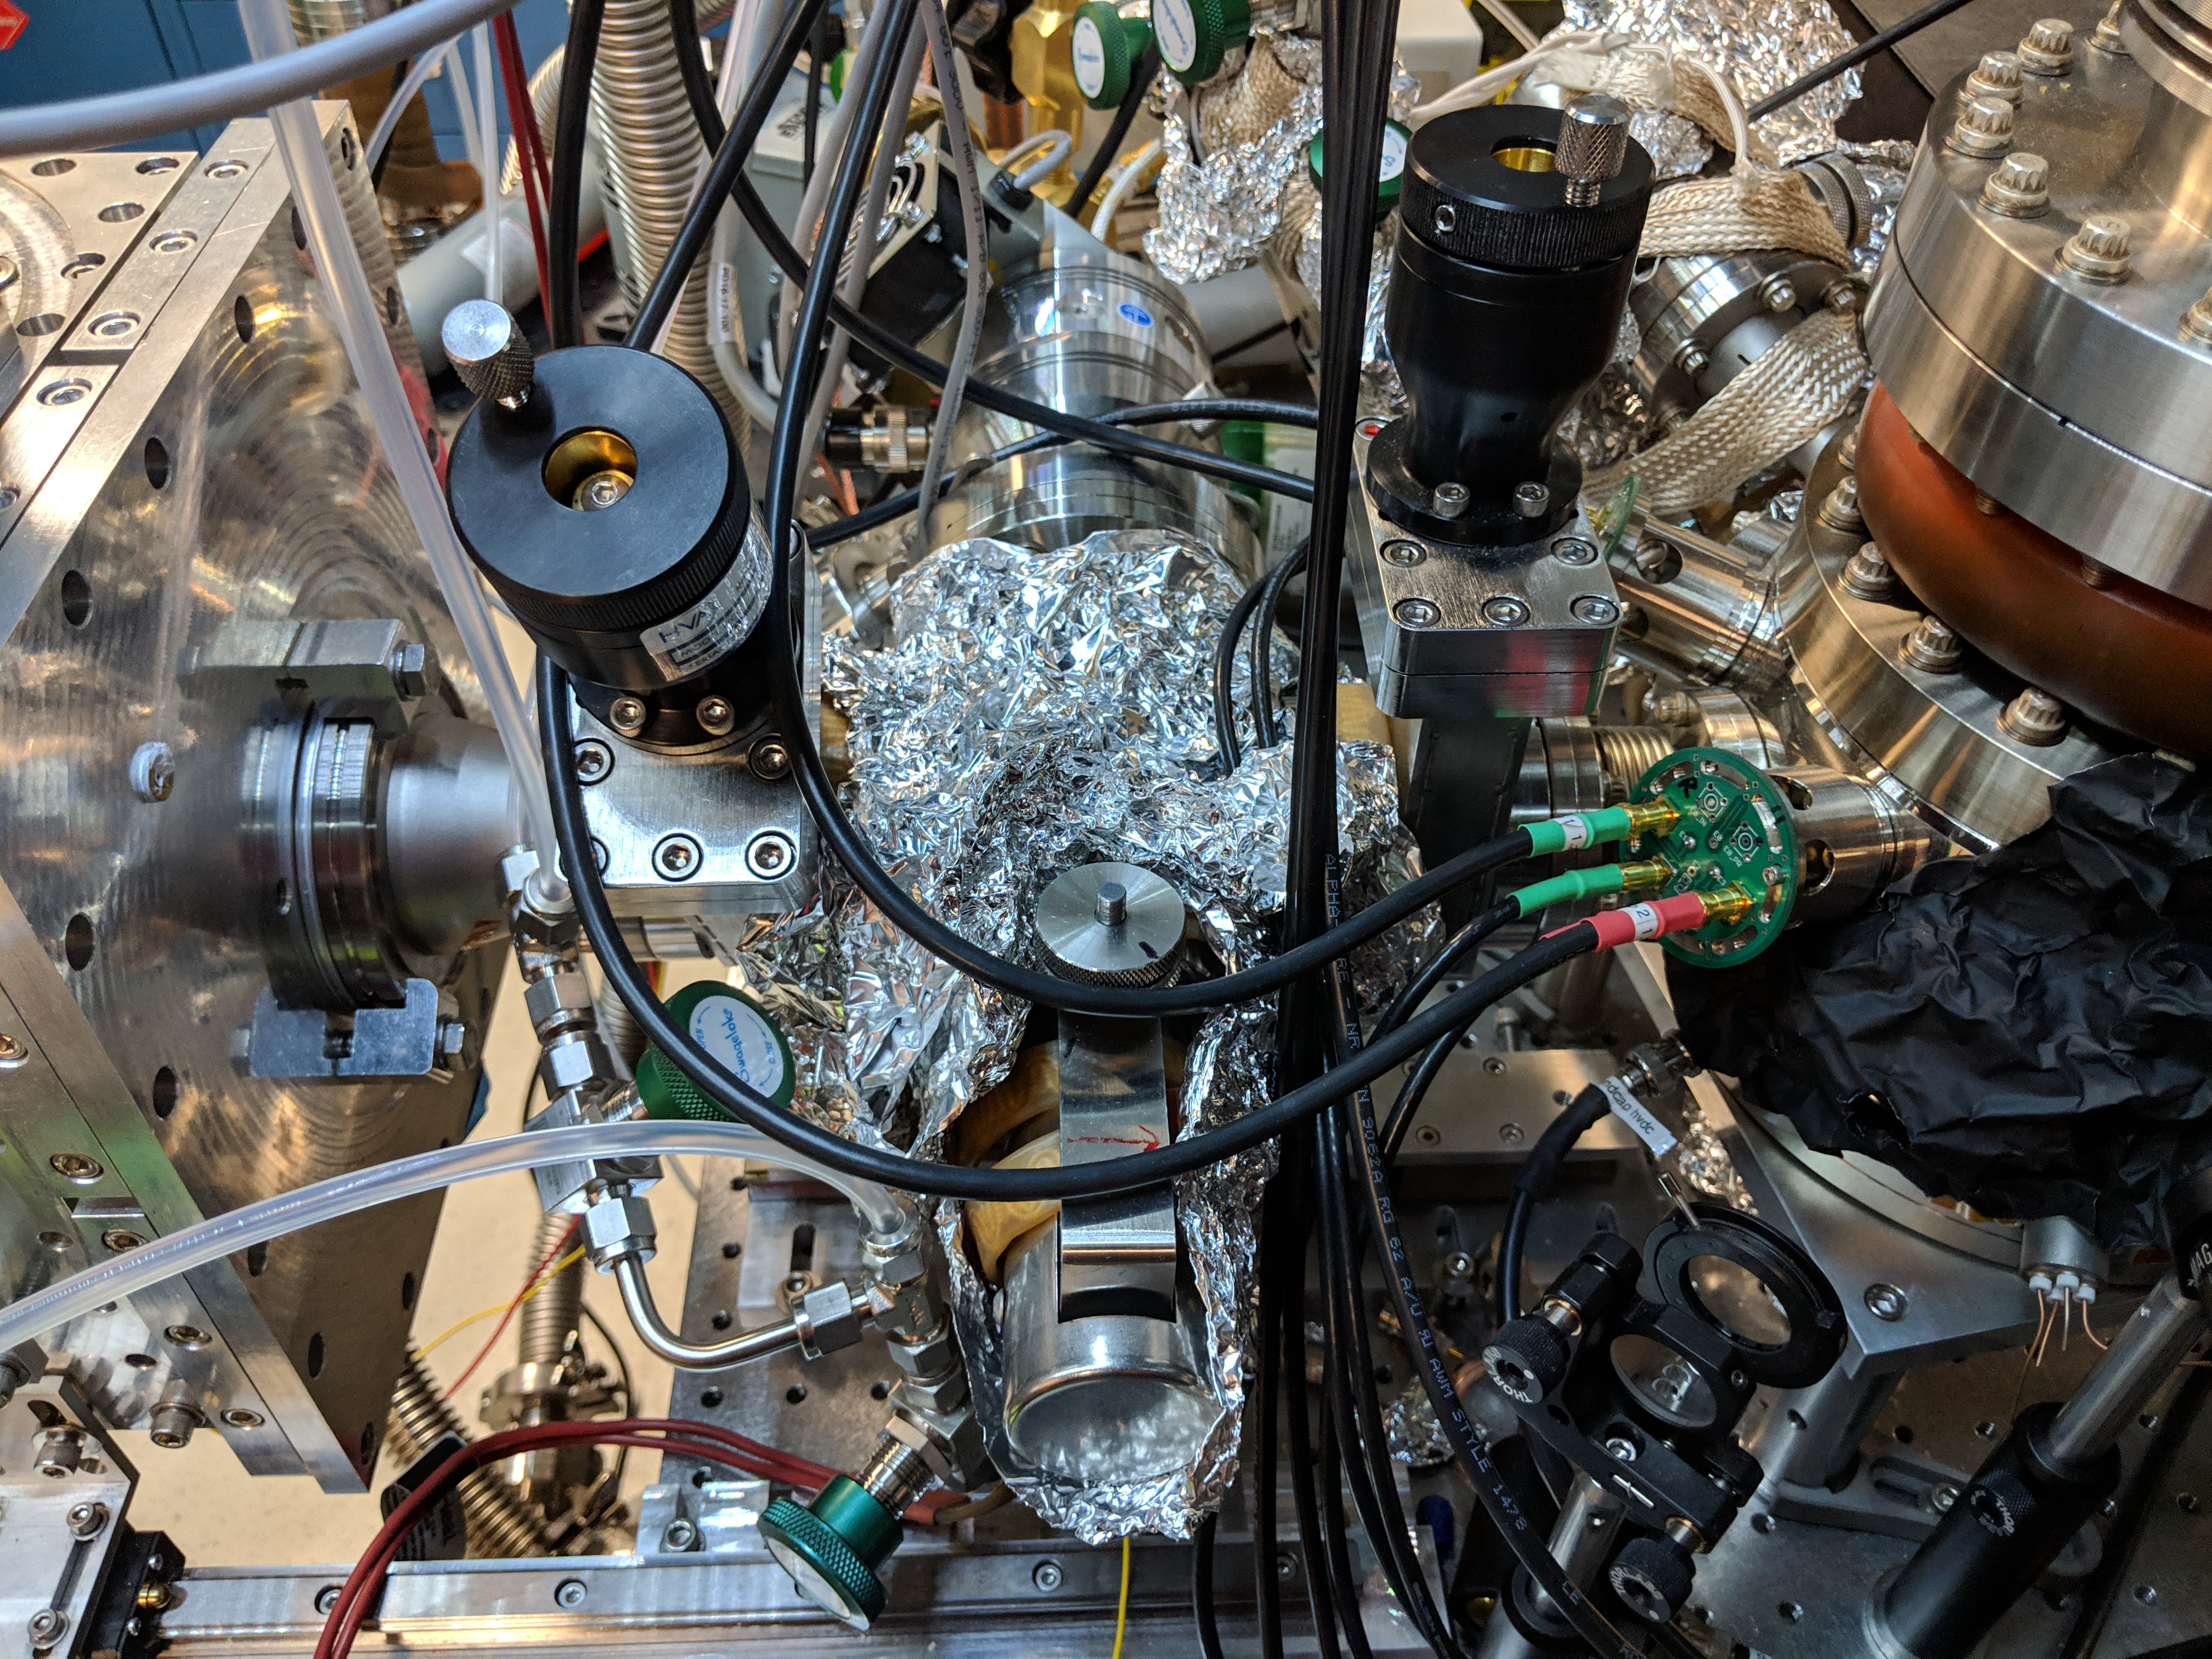
\includegraphics[width=0.8\textwidth]{images/differential_pumping.jpg}
	\caption{Differential pumping region in between the stem and ion trap chambers with gate valves on either end. Blank copper CF gaskets with apertures of 4 mm and 10 mm are placed towards the stem and ion chamber respectively to limit conductance of background gasses while allowing the cryogenic beam through. An Agilent Twistorr 84 FS turbo pump keeps the region at pressures around $10^{-10}$ Torr and a leak valve allows for controlled introduction of secondary gasses.}
\end{figure}
	
	\section{\ce{^9Be+} Laser Cooling}
	Laser cooling for the \ce{^9Be+} ion is done with a Toptica TA-FHG Pro tuned to 313 nm with a peak power of 400 mW. The fundamental laser light is blue-detuned by 400 MHz from the \ce{^2S1/2} to \ce{^2P3/2} transition. The fundamental is then passed through a 400 MHz AOM to be on resonance with the transition. The unperturbed light is then double passed through another 400 MHz AOM to repump the population that has fallen into the \ce{2S1/2} state.

\begin{figure}[H]
	\centering
	\missingfigure{Be electronic structure}
	\caption{Electronic structure of \ce{^9Be+}, laser cooling is done with 313 nm light.}
\end{figure}

\begin{figure}[H]
	\centering
	\missingfigure{Laser and AOM's}
	\caption{AOM's running at 400 MHz are used to tune the initially blue detuned primary beam on resonance with the \ce{^2S1/2} to \ce{^2P3/2} transition. A double passed AOM tunes the primary beam to the \ce{^2S3/2} to \ce{^2P3/2} transition to re-pump any \ce{^2P3/2 -> ^2S3/2} decays. A third AOM creates a first order beam 200 MHz red to aid the capture of hot ablated \ce{Be+} ions.}
\end{figure}

As we excite the cooling transition, force is being imparted onto the ion via absorption of the photons and spontaneous emission. We can define the force to be the product of the scattering rate of a two level system and the momentum of each photon.

\begin{align}
	F & = p \Gamma \rho_{pp} \nonumber \\
	& = \hbar k \Gamma \frac{1}{2} \frac{s}{1+s+4\left(\frac{\delta-\vec{k}\cdot \vec{v}}{\Gamma}\right)^2} \label{eq: laser force}
\end{align}

Where $k$ is the photon's wavenumber, $\Gamma$ is the linewidth of the excited transition, and $\rho_{pp}$ is the probability of finding the ion in the excited \ce{^2P3/2} state characterized by the saturation parameter $s = I/I_s=I/(\frac{\pi h c}{3 \lambda^3 \tau})$ and laser detuning $\delta=\omega_0-\omega_l$. We can see that the force the ion feels is dependent on the laser detuning from resonance, which in turn is dependent on the doppler shift of the ion with respect to the laser $\vec{k} \cdot \vec{v}$. In general, the laser frequency ($\omega_l$) is red detuned from the cooling transition ($\omega_l < \omega_0$). In this instance, if the ion is moving towards the laser such that the velocity ($v$) and $k$ vector are anti-aligned, we see a positive doppler shift in the frequency ($+kv$), decreasing the effective detuning, increasing the scattering rate. When the ion is moving away from the laser while $\omega_l < \omega_0$ is true, we see that the detuning increases, lowering the scattering rate. Each time the ion absorbs a photon, it gains a momentum kick in the photon's direction, meaning the ion preferentially absorbs light that causes it to lose momentum. After absorption, the ion emits a photon after $\tau=\Gamma^{-1}$ time, isotropically, which averages to zero. We can Taylor expand equation \ref{eq: laser force} for small values of $v$ to find this velocity dependence.

\begin{equation*}
	F(v) = F(v=0) + \beta v
\end{equation*}

Where we define the damping coefficient:

\begin{equation*}
	\beta= 4 \hbar k^2 \frac{s \frac{\delta}{\Gamma}}{1+s+4\left(\frac{\delta}{\Gamma}\right)^2}
\end{equation*}

Since the ion trap is not a perfect harmonic potential, which would require hyperbolic trap electrodes, the ion's trajectory is mixed along each axis, allowing for the 3 dimensional laser cooling with just one beam angled from both radial and axial axes of the trap.
	
	\section{Imaging System}
	Using the 313 nm laser, we fluoresce the \ce{Be+} ions and cool them down to a cloud or crystal in the ion trap. The scattered light is observed via our imaging system shown in Figure \ref{fig: imaging system}. The components include the Andor iXon3 camera with EM gain, a 313 nm band pass filter, angled mirror, enclosing lens tubes, and Sill objective lens with 0.2 NA, and 40 mm working distance. The alignment of our objective lens to camera imaging plane yields a magnification of about $\times5.5$. All of the imaging components are rigidly mounted onto the 3 axis translation stage allowing us to move the focal point without changing the magnification. The total efficiency of our imaging system is
\begin{equation}
	\epsilon = \Omega \alpha \beta \gamma
	\label{eq: fluorescence efficiency}
\end{equation}
where $\Omega$ is the solid angle the reentrant objective appends, $\alpha$ is the camera's quantum efficiency at 313 nm, $\beta$ is the camera's exposure time, and $\gamma$ is the camera's gain. For a fluorescing ion scattering at $\Gamma \times (\rho_{pp} \approx 0.20)$, we expect on the order of $10^5$ counts per ion after the imaging inefficiencies.

With images of the ion clouds used in our chemical reaction studies, approximate the temperature of the ions by assuming they are in a harmonic potential. In the same fashion that we derived the trap depth, we may find a characteristic temperature of the ion cloud in the trap from the spacial width. With a very large cloud of ions that are not in a Coulomb crystal, we estimate a maximum temperature of 500 mK by estimating the physical width of the ion cloud. When compared to the temperature of a gas introduced via leak valve or even the CBGB, the ions in the trap may be considered to effectively have zero velocity.

\begin{figure}[H]
	\centering
	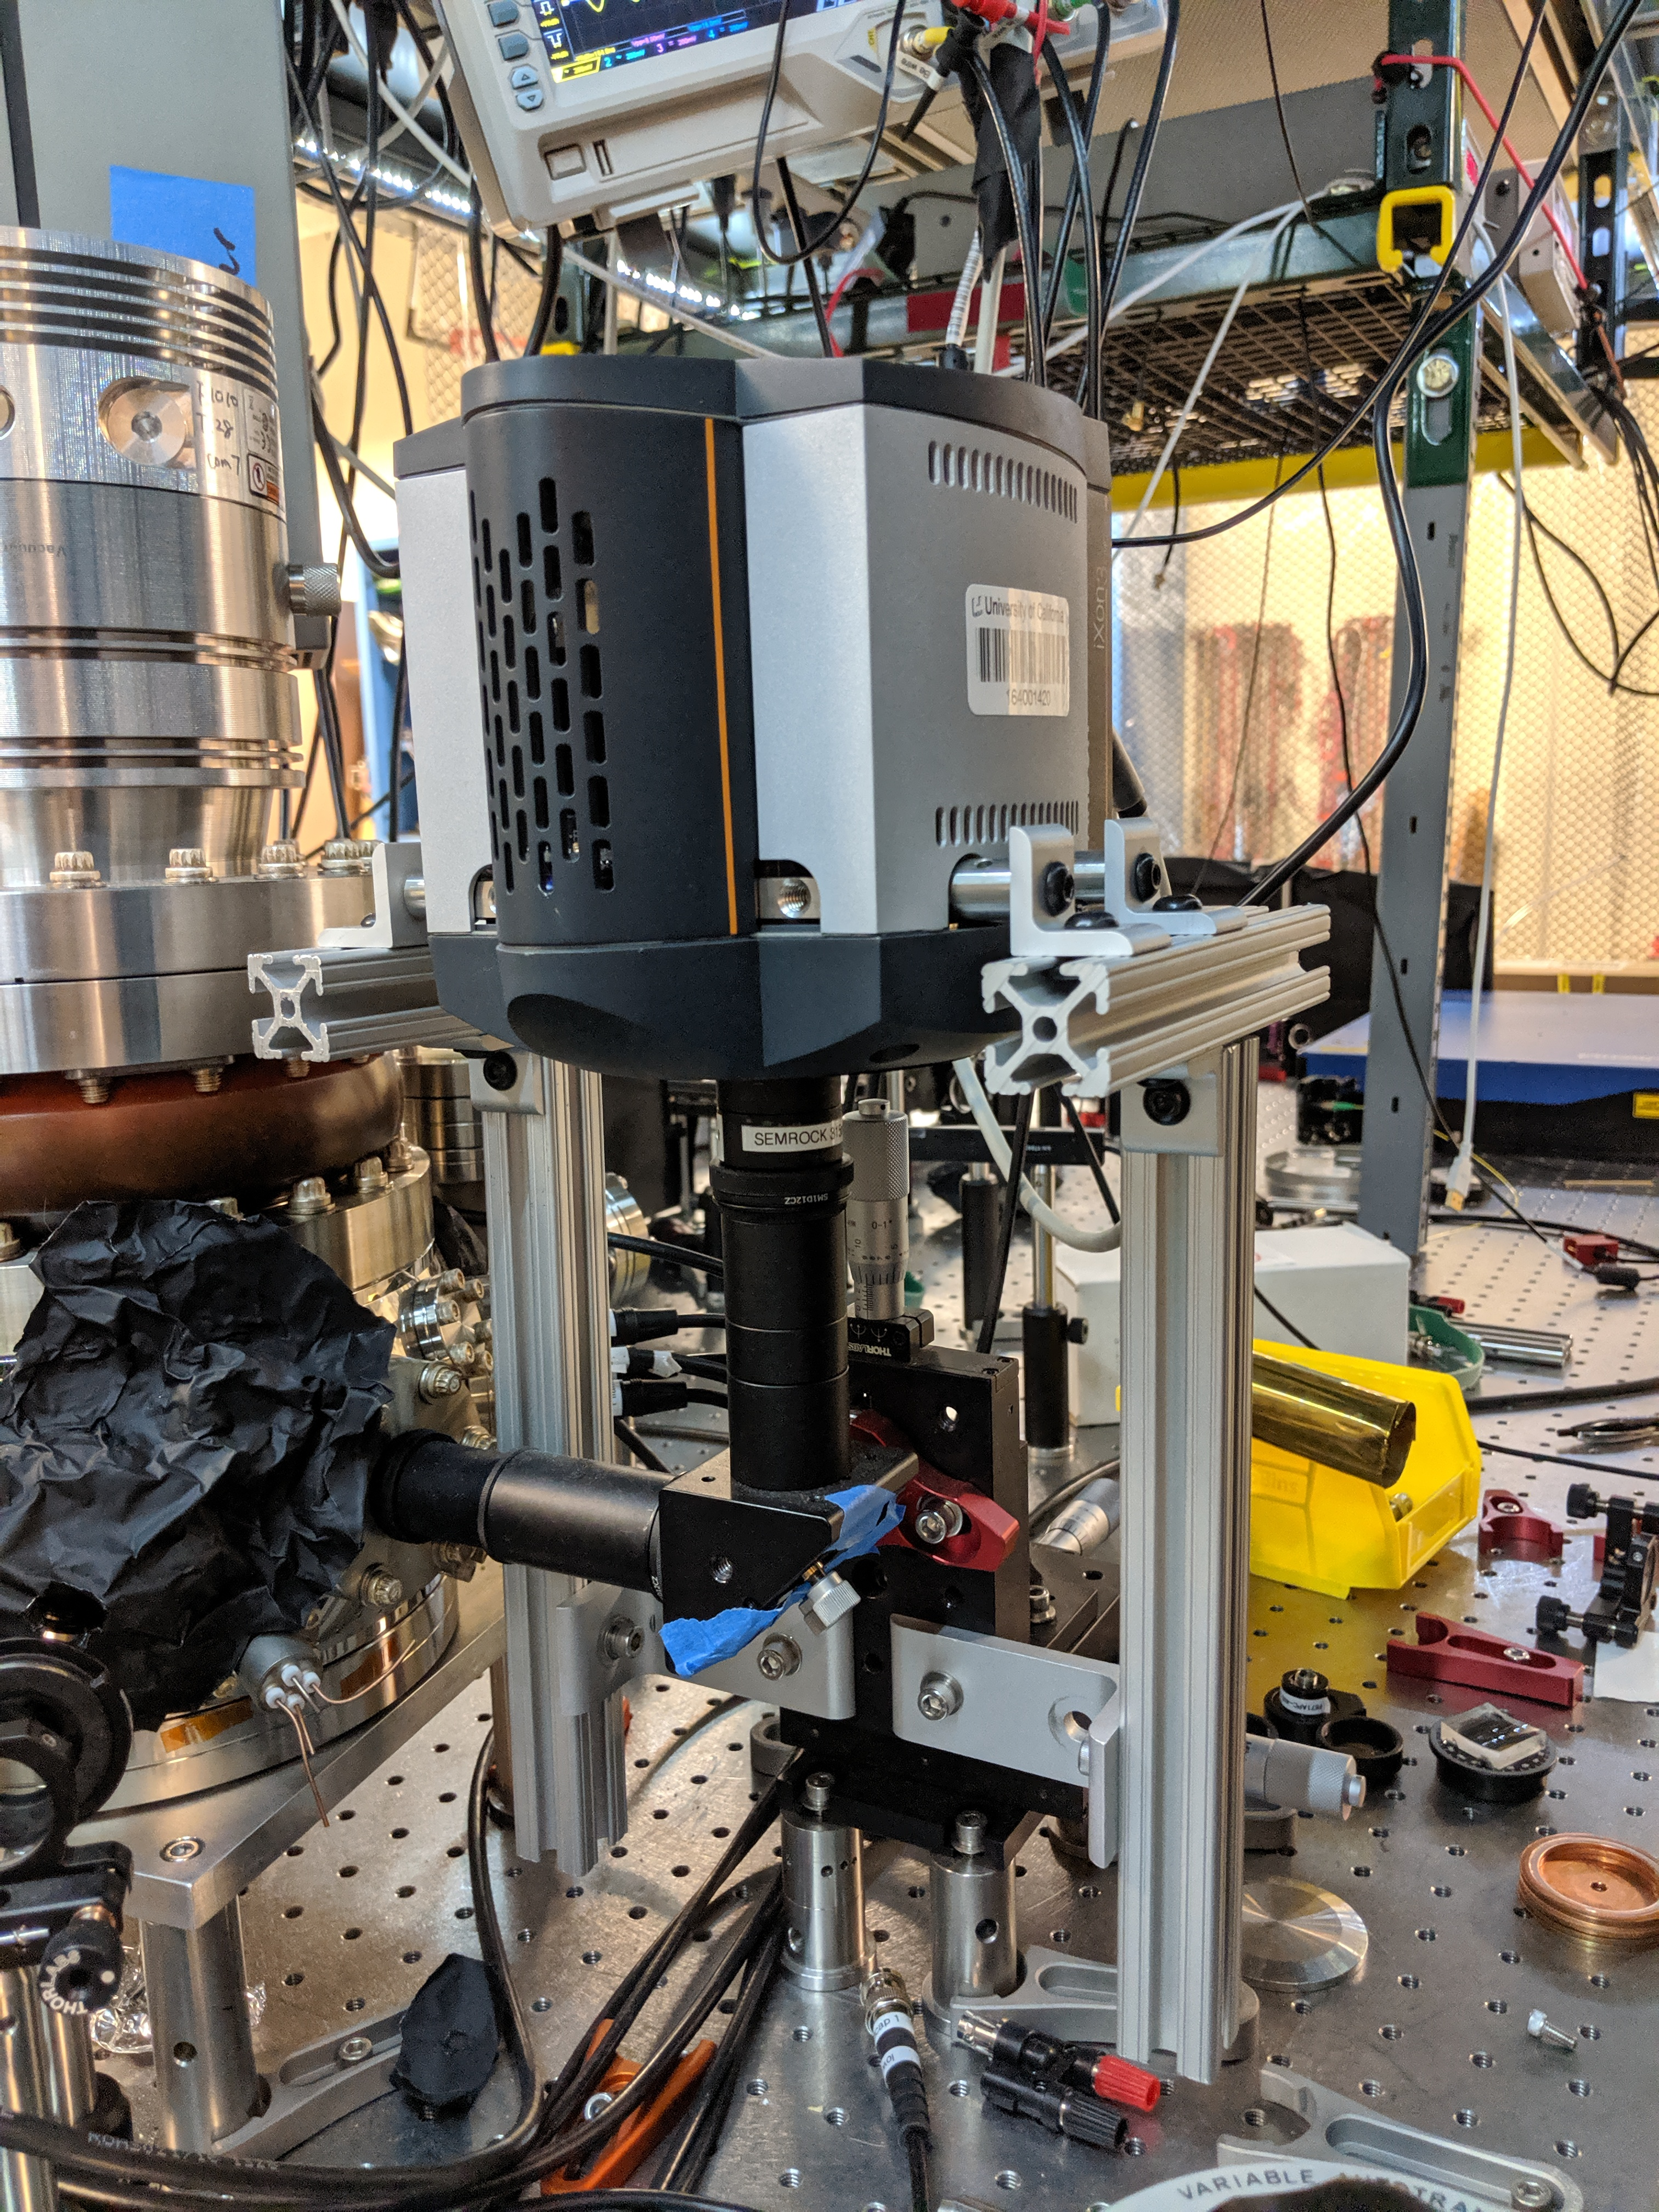
\includegraphics[height=0.8\textwidth]{images/imaging_system.jpg}
	\caption{The Andor iXon3 camera, enclosed imaging pathway, and objective lens are all mounted onto a 3 axis translation stage. The Sill objective lens is mounted at then end of the imaging tubes, inserted into the reentrant flange. An angled mirror directs the light at a 90$^\circ$ angle up and through a 313 nm bandpass filter placed in front of the camera sensor.}
	\label{fig: imaging system}
\end{figure}

\begin{figure}[H]
	\centering
	\includegraphics[width=0.8\textwidth]{images/ion_crystal.png}
	\caption{Laser cooled Coulomb crystal of \ce{Be+} ions in the LQT imaged with the reentrant imaging system. Dark \ce{BeH+} ions are sympathetically cooled in the middle of the top row as well as the third position from the right.}
	\label{fig: ion crystal}
\end{figure}
	
	\section{Determining Excited State Population}
	Ideally, having a single ion in the trap while sweeping the frequency or power would allow us to determine the saturation parameter, and thus the fraction of \ce{Be+} in the excited \ce{^2P3/2} state. Due to the size and depth of our ion trap, we cannot reliably load only one ion. On top of that, the most common residual gasses in a vacuum chamber, \ce{H2O} and \ce{H2} both readily react with \ce{Be+} in the excited state. Instead, we take images of the ions at various powers and find the fluorescence per ion to fit to a generalized form of the scatter rate ($\Gamma_d$):

\begin{align}
	\Gamma_d & = a \rho_{pp} \nonumber \\
	& = \frac{a}{2}\frac{s}{1+s+4(\delta/\Gamma)^2} \label{eq: fluor fit}
\end{align}

Where the parameter $a$ consists of all the efficiency parameters in equation \ref{eq: fluorescence efficiency}. To get the P-state fraction, \ce{Be+} ions are loaded into the trap and A-ramps are applied until a chain is formed and the laser detuning adjusted until we see maximum fluorescence on the camera, which coincides with a detuning of $\Gamma/2$. Then images of the ions are taken at various laser powers and run through a maximum filter algorithm to identify the locations of individual ions as seen in figure \ref{fig: ion image set}. The portion of the image not an ion is then averaged to obtain the background pixel value, which is then subtracted from each localized ion image. The pixel values over each localized ion is then summed to yield a total fluorescence value, which is then averaged for each image as shown in figure \ref{fig: local ions}. By fitting the collected fluorescence per ion as a function of incident power, we find the generalized efficiency $a$, revealing the P-state fraction at each power in $\rho_{pp}$, shown in figure \ref{fig: p state curve}.

\begin{figure}[H]
	\centering
	\includegraphics[width=0.8\textwidth]{images/ion_images.png}
	\caption{A set of ion images taken at various 313 nm powers run thorough a maximum filter algorithm that identifies local maxima, representing individual ions (circled in red).}
	\label{fig: ion image set}
\end{figure}

\newpage
\begin{figure}[H]
	\centering
	\includegraphics[height=0.7\paperheight]{images/isolated_ions.png}
	\caption{Individual ions identified from images in figure \ref{fig: ion image set}. Integrated pixel values with subtracted background counts shown for each image, a set's averaged value is shown in brackets.}
	\label{fig: local ions}
\end{figure}

\begin{figure}[H]
	\centering
	\includegraphics[width=0.8\textwidth]{images/P_state_curve.png}
	\caption{P-state fraction curve fitted to incident laser power at a fixed detuning of $\delta = \Gamma/2$. Total fluorescence value is normalized by fitted efficiency parameter $a$ to yield $\rho_{pp}$.}
	\label{fig: p state curve}
\end{figure}

	\section{Time of Flight Mass Spectrometer (TOF-MS)} \label{sec: TOF}
	One of the key components of this experiment is the fact that charged reaction products stay within the ion trap, allowing us to accumulate all stages of a reaction network. Direct identification of the species via fluorescence is ideal, as the signal is unambiguous, and generally unique to a species. Leaning on direct fluorescence becomes increasingly difficult as more and more species are introduced. In our particular case, it becomes prohibitively difficult, as we may expect to trap 10's of species at once, where in some cases, the exact reaction products are not known. To identify what is in our trap, we use a species agnostic detection method in the form of a time of flight mass spectrometer (TOF-MS). Our TOF apparatus design and electronics were extensively developed by Steven Schowalter and Christian Schneider of the Hudson group.\cite{Schowalter2012,Schneider2014}

The TOF works by switching the rod voltages from a trapping RF potential to one where the ions are ejected out of one side. When trapping, RF voltages are applied onto diagonal rods, while DC voltages on the others. During ejection, the trapping region turns into the acceleration region as adjacent pairs of rods ramp to constant voltages where the pair of "back" rods are at a higher potential than the pair of "front" rods seen in Figure \ref{fig: rod traces}. TOF's operating with higher $m/z \approx>100 $ need to have well matched HVDC values for the rods, without much concern over the rising voltages. In our experiment, due to the low $m/z$ of \ce{Be+}, the ions were extremely susceptible to mismatches in the rod voltages during the ramp up, requiring particularly good overlap seen in $\sim 0.8 - 1.2$ $\mu$s of Figure \ref{fig: rod traces}

\begin{figure}
	\centering
	\includegraphics[width=0.8\textwidth]{images/rod_traces.pdf}
	\caption{Voltages of ion trap rods during ejection into the TOF taken from an oscilloscope. TOF facing front (1 and 3) and back (2 and 4) trap rod pairs shift from the trapping RF operation to HV values after a positive zero voltage crossing. The front pair reaches a nominal 1000 V, while the back pair reaches 1400 V, creating an accelerating potential $\Delta V$, ejecting the trapped ions.}
	\label{fig: rod traces}
\end{figure}

\begin{figure}
	\centering
	\includegraphics[width=0.8\textwidth]{images/TOF_diagram.pdf}
	\caption{Diagram of the TOF ejection where the ions in the trap are radially accelerated out of the trap with potential $\Delta V$. An Einzel lens ion focusing element focuses the ions onto the MCP at the back of the field free region of length $D$.}
	\label{fig: TOF diagram}
\end{figure}

As the ions are ejected radially, they are accelerated out of the trap, through an Einzel lens focusing element, and through a field-free drift tube of length $D=320$ mm where they impact a micro-channel plat (MCP) and are detected (Figure \ref{fig: TOF diagram}). To first order, during ejection the ions in the ion trap feel the same potential $\Delta V$, therefore, the same kinetic energy
\begin{equation*}
	\Delta V q = \frac{1}{2} m v^2.
\end{equation*}
But solving for the velocity $v$ yields a mass dependent velocity, thus, a mass dependent arrival time $t$,
\begin{align*}
	v & = \sqrt{\dfrac{2 \Delta V q}{m}} \\
	\implies t & = D \sqrt{\dfrac{m}{2 \Delta V q}}.
\end{align*}
With fast electronics, we may resolve ions to sub amu precision, giving us a powerful tool to identify what is in our trap. An example of \ce{Be+} and \ce{C+} TOF detection traces is shown in Figure \ref{fig: Be C TOF} with a ratio $m/\Delta m \approx 100$.

To first order, the mass to charge ratio ($m/z$) is then proportional to $t^2$ where $t$ is the arrival time, which is proportional to the drift tube length $D$. It may seem like greater mass separation is achieved with a longer drift tube, but that is not the case. We made the assumption that the ions are accelerated by the same potential, but in reality, the ions occupy a finite spacial extent in which the potential felt by an ion is related to its location within the trapping region at the time of ejection. An ion in the center of the trap at the time of ejection will have a distance $d_0\approx 4.8$ mm to travel in the acceleration region, while those towards the back/front pair of rods will have distances $d=d_0\pm \delta d$. As these ions fly down the drift tube, although the ions initially closer to the front have a shorter distance to travel, the ones originating further back have a higher velocity and will catch up and over take the slower ions. This mismatch will cause the ion arrival times of a single species to spread out as $D$ increases past the point where all the ions overlap.

On top of considering the spacial extent of the ions in the trap, we must also consider the multiple acceleration regions. The rods that the trap consists of produce a fairly uniform electric field within the trap region $E_d$, but outside, there is still an accelerating electric field $E_s$, but primarily from the front rods. To minimize the ion defocusing at the MCP, we find that the drift tube length $D$ is uniquely defined by the trap geometry and voltages,\ref{Wiley1955}
\begin{equation}
	D = 2d_0 k_0^{3/2}\left(1-\frac{1}{k+\sqrt{k}}\right)
\end{equation}
where $k = (E_s + E_d)/E_s$.

\subsection{TOF Signal Integration}

The MCP detector produces a current proportional to the number of ions that activate its surface, which is then read by a fast oscilloscope. To determine the total number of ions, we integrate the current as a function of arrival time to find a total charge for each calibrated amu range (colored regions in Figure \ref{fig: Be C TOF}). A difficulty is determining whether or not an integrated peak corresponds to an ion, or simply noise. For each TOF trace, we find a region of high mass (e.g. $m/z > 45$), where there aren't any ions and bin single amu chunks to produce a histogram. This histogram is then fitted to a Gaussian to determine the standard deviation, where then we may find a 90\% confidence interval ($\approx 1.3 \sigma$). This value then defines our signal threshold, if an integrated signal is below this value, it is rejected and a zero is returned with error bars equal to this threshold, otherwise it is reported as a true ion signal.
	
	\section{Dual Species Loading} \label{sec: dual loading}
	Although loading and cooling \ce{Be+} ions is fairly straight forward, it is not as clear as how to load \ce{C+} ions into the trap with \ce{Be+} reliably. Early attempts involved using the home-made electron gun to dissociate \ce{CO} gas introduced via leak valve, where all possible ionized products of \ce{CO} were detected (\ce{C+}, \ce{O+}, and \ce{CO+}). Even when loading into an empty trap, it was not possible to reliably isolate the \ce{C+} via A-ramping of the trap RF voltage. Prolonged use of the electron gun directly towards the ion trap also caused charging that would slowly dissipate and change the trap parameters. On top of these complications, it would not have worked in conjunction with ablation loading \ce{Be+}, as these cannot occur simultaneously.

Instead of using two different methods to load the different ion species, ablating samples of both species simultaneously was found to be the best method. A sample of \ce{Be} metal was placed on top of a piece of graphite on the target holder so that both samples were in view of the ablation laser. The set up shown in figure \ref{fig: dual ablation} allowed us to separate the Minilite ablation laser into two beam with independent alignment and focal planes. The polarization of the laser light is rotated with a half-waveplate, which then enters a polarizing beam splitter (PBS), allowing for tuning of power into either path. The vertically polarized reflected light is reflected off a second PBS and is steered up to the objective lens and then focused into the chamber. The horizontally polarized light transmitted through the first PBS is aligned through an adjustable telescope system. This light is then realigned with the vertically polarized light on the second PBS, co-propagating into the chamber. This "delay stage" for the horizontal light allows for independent focusing and alignment onto a target.

\begin{figure}[H]
	\centering
	\includegraphics[width=\textwidth]{images/ablation_optics.png}
	\caption{Image of the single laser, dual ablation set up. The 1064 nm YAG pulse is split into two paths, and recombined such that they proceed through the same focusing element into the chamber to hit two different targets. Leg a) is used for the ablation of graphite to produce \ce{C+}, while leg b) is independently focused and positioned to ablate beryllium metal to produce \ce{Be+}.}
	\label{fig: dual ablation}
\end{figure}

Blocking one beam allowed for adjustments for the ablation of each species independently. When loading \ce{C+}, we found a strong dependence of the trapped species and the fluence. Lower fluence created not only \ce{C+}, but clusters of, \ce{C2+}, and \ce{C3+} as well. Tight focusing of the beam improves the efficiency of creating only \ce{C+}, but some \ce{Cn+} is still usually produced. By changing the trap's $a$ parameter (A-ramp) via changing the $V_{DC}$ (\ref{eq: a param}), we can change the stability diagram for the trap, causing higher $m/z$ ions to become more unstable. The higher mass \ce{Cn+} ions are preferentially kicked out of the trap, while the lighter \ce{Be+} and \ce{C+} are less affected, allowing us to load clean samples of the desired species.

\begin{figure}[H]
	\centering
	\includegraphics[width=0.8\textwidth]{images/Be_C_TOF.png}
	\caption{TOF trace of simultaneous \ce{Be+} and \ce{C+} ablation loading averaged over 10 shots. A soft A-ramp is applied after loading, ejecting any unintentionally loaded \ce{Cn+} clusters. The \ce{C+} peak is narrowed from sympathetic cooling with the laser cooled \ce{Be+} ions.}
	\label{fig: Be C TOF}
\end{figure}

An important consideration is that that the amount of ions loaded from shot-to-shot is not identical; the amounts may be similar, but can drift over time, especially for the \ce{C+} peak, as the ablation of graphite is less reliable as beryllium metal. As we run experiments, which can take upwards of 200 shots to complete, we cannot make assumptions on the total number or ratio of loaded ions. With \ce{Be+}, we may use the camera in conjunction with the TOF and normalize the total \ce{Be+} reaction network with the fluorescence. Because the \ce{Be+} fluorescence has no indication on the amount of \ce{C+} loaded into the trap, the \ce{C+} reaction network must then be normalized separately for total ion count in each division.

\chapter{Optical Control of Reactions between Water and Laser-Cooled \ce{Be+} Ions} \label{sec: Be+H2O}
%%	% !TEX root = ../thesis.tex
\subsection{Abstract}
We investigate reactions between laser-cooled \ce{Be+} ions and room-temperature water molecules using an integrated ion trap and high-resolution time-of-flight mass spectrometer. This system allows simultaneous measurement of individual reaction rates that are resolved by reaction product. The rate coefficient of the \ce{Be+(^2S1/2) + H2O -> BeOH+ + H} reaction is measured for the first time and is found to be approximately two times smaller than predicted by an ion-dipole capture model. Zero-point-corrected quasi-classical trajectory calculations on a highly accurate potential energy surface for the ground electronic state reveal that the reaction is capture-dominated, but a submerged barrier in the product channel lowers the reactivity. Furthermore, laser excitation of the ions form the \ce{^2S1/2} ground state to the \ce{^2P3/2} state opens new reaction channels, and we report the rate and branching ratio of the \ce{Be+(^2P3/2) + H2O -> BeOH + H} and \ce{H2O} + Be reactions. The excited-state reactions are nonadiabatic in nature.

\subsubsection{Introduction}

Low-temperature reactions of simple ions with small molecules play a central role in astrochemical environments from interstellar clouds to cometary comae to planetary atmospheres, including that of Earth\cite{Agundez2013,Krasnopolsky2014}. The chemical evolution of interstellar molecular clouds ultimately yields the seedbed from which new stars and planets are born and the raw materials from which life likely developed. A firm understanding of the reaction rates for a host of elementary ion-molecule reactions is essential to accurately model these environments these environments. Techniques such as selected ion flow tubes (SIFTs)\cite{Adams1976}, guided ion beams\cite{Armentrout2002}, and supersonic flows (CRESU)\cite{Sims2002} have improved our empirical understanding of these processes; however, each has its own limitations.\cite{Smith2000,Snow2008} Theoretically, it has long been recognized that these ion-molecule reactions are often barrierless, and their rates are frequently described by capture models.\cite{Gioumousis1958a} However, recent studies have revealed that dynamical features can sometimes prevail,\cite{Lourderaj2008,Li2014,Carrascosa2017} in which case statistical treatments may not be accurate.\cite{Hase2014,Clary1990} Therefore, new experimental and theoretical efforts are needed to accurately address ion-molecule chemistry.

We have developed an approach, adapted from the ultracold ion community,\cite{Hudson2016,Tomza2017,Willitsch2012a} to study reactions of atomic ions with small molecules. Here we report the use of this approach to study the reaction of \ce{Be+} with gas=phase water for the first time. There have been very few experimental studies of gas-phase reactions between metal ions and water, especially at low temperature, despite their importance for metal ion chemistry in a range of environments.\cite{Highberger2001,Oppenheimer2002,VanDishoeck2013a}

Singly ionized beryllium is a particularly attractive metallic reactant to use for such studies because it is both theoretically tractable and experimentally highly controllable. The relatively simple electronic structure of this three-electron ion allows both highly accurate characterization of its electronic structure and laser cooling,\cite{Bollinger1985} and the low mass of \ce{Be+} lends itself to high motional frequencies as well as efficient sympathetic cooling of other chemically interesting atomic ions when employed in ion traps.\cite{Chen2014a,Roth2006,Larson1986,Schowalter2016} For the molecular reaction partner, \ce{H2O} is arguably the most important molecule in chemistry, and theoretical studies of its reactions with a single atom have been reported on full-dimensional potential energy surfaces (PESs).\cite{Li2013,Song2015,Ray2017,Li2015,Xiao2011} Thus this system of reagents provides an opportunity to perform a high-resolution comparison between experiments and theory for a molecule-ion system.

The apparatus employed here is shown in the Supporting Information (SI) (Figure S1). Laser ablation of metallic \ce{Be} is used to produce \ce{Be+} ions, which are trapped in a linear radio frequency Paul trap.\cite{Wolfgang1990} Laser cooling \cite{Wineland1979} is used to cool the translational motion of the ions, resulting in a Coulomb crystal of \ce{Be+} ions. Gaseous, room-temperature \ce{H2O} molecules are then introduced via a leak valve into the trapping region, where they react with the trapped ions. Charged products of the chemical reaction remain in the trap and are subsequently detected via an integrated time-of-flight mass spectromemter (TOFMS) recently developed by our group\cite{Schowalter2012,Schneider2014} and used to discover new species.\cite{Puri2017} The total reaction rate is measured by monitoring the decay of \ce{Be+} ion fluorescence, and the product branching ratios are extracted from the mass spectrum.

A key feature of this experiment is that by varying the detuning of the 313 nm laser used to cool the ions, the population in the excited \ce{1s^2 2p^1 ^2P3/2} and ground \ce{1s^2 2s^1 ^2S1/2} states can be controlled. Because the energy difference between the ground and excited states is 3.96 eV, several more product channels are open for the \ce{Be+(^2P3/2) + H2O} entrance channel. Using this system, we are able to measure the reaction rate and product branching ratio for these two entrance channels. We find that the ground-state channel, \ce{Be+(^2P3/2) + H2O}, exclusively produces \ce{BeOH+ + H}, whereas the excited-state channel, \ce{Be+(^2P3/2) + H2O}, also produces \ce{H2O+ + Be} with a yield of $~10\%$. Specifically, the reactions considered here are

\begin{align}
	\ce{Be+(^2S1/2) + H2O & -> BeOH+ + H} \label{r: Be(S)+H2O->BeOH} \\
	\ce{Be+(^2P3/2) + H2O & -> BeOH+ + H} \label{r: Be(P)+H2O->BeOH} \\
	\ce{Be+(^2P3/2) + H2O & -> H2O+ + Be} \label{r: Be(P)+H2O->H2O} \\
	\ce{H2O + H2O+ & -> H3O+ + OH} \label{r: H2O+H2O->H3O} \\
	\ce{Be+(^2P3/2) + H2O & -> BeH+ + O2} \label{r: Be(P)+H2O->BeH} \\
	\ce{BeH+ + H2O & -> BeOH+ + H2} \label{r: BeH+H2O->BeOH} \\
	\ce{Be+(^2P3/2) + H2O & -> BeO+ + H2} \label{r: Be(P)+H2O->BeO} \\
	\ce{BeO+ + H2O & -> BeOH+ + OH} \label{r: BeO+H2O->BeOH}
\end{align}

Because the translational energy of the laser-cooled \ce{Be+} ions is $<0.5$ K, the energy of the room-temperature water sets the reaction kinetic energy of \ce{Be+ + H2O} in the center of mass frame fo $~100$K. The internal state distribution of the \ce{H2O} is assumed to be given by the 300 K. Typical TOF traces (10 sample average) at reaction times $t=0$ and 70 s with 7 and 26\% relative \ce{Be+(^2P3/2)} state excitation are shown in Figure 1A,B, respectively. The fluorescence signal, which is used to determine the reaction time zero and normalize the initial ion number for the TOF, is monitored by the camera (ANDOR iXON3 EMCCD) in real time. At $t=0$ s, a large peak of $m/z=9$(\ce{Be+}) and a smaller one of $m/z=9$(\ce{BeOH+}) are evidenced in the TOF trace (blue line), which indicates that \ce{Be+} ions are the main species in the trap at $t=0$. The finite amount of \ce{BeOH+} at $t=0$ reflects the fact that reactions \cref{r: Be(S)+H2O->BeOH,r: Be(P)+H2O->BeOH,r: Be(P)+H2O->H2O,r: H2O+H2O->H3O,r: Be(P)+H2O->BeH,r: BeH+H2O->BeOH,r: Be(P)+H2O->BeO,r: BeO+H2O->BeOH} happen even during the loading process and that the mass filtering procedure is imperfect. At $t-70$ s, a $m/z=19$ peak emerges when more \ce{Be+} ions are excited to \ce{^2P3/2} state\todo{ref figure}, which we identify as \ce{H3O+} resulting from reactions \cref{r: Be(P)+H2O->H2O,r: H2O+H2O->H3O}. The \ce{BeOH+ / H3O+} ratio, $\eta(P_\text{P})$, is measured by integrating both peaks for the experimentally controlled excited-state population $P_\text{P}$. The \ce{BeOH+} signal includes the amount unfiltered during loading, products from both reactions \cref{r: Be(S)+H2O->BeOH,r: Be(P)+H2O->BeOH}, as well as, in principle, the two-step reactions \cref{r: Be(P)+H2O->BeH,r: BeH+H2O->BeOH,r: Be(P)+H2O->BeO,r: BeO+H2O->BeOH}. The \ce{H3O+} signal is produced via the two-step reactions \cref{r: Be(P)+H2O->H2O,r: H2O+H2O->H3O}. Whereas we do not observe products from reactions \cref{r: Be(P)+H2O->BeH,r: BeH+H2O->BeOH,r: Be(P)+H2O->BeO,r: BeO+H2O->BeOH} (see also \todo{ref figure} in SI), they are thermochemically allowed and therefore included in our analysis, which sets upper limits on their reaction rate coefficients.

The total reaction rate is given by $\Gamma_t = \rho_{\ce{H2O}} k_t$, where $\rho_{\ce{H2O}}$ is the \ce{H2O} density measured from a Stanford Research Systems residual gas analyzer (RGA) calibrated to an ion gauge (see the SI for more information) and $k_t$ is approximated as $k_t = P_\text{S} k_1 + P_\text{P} k_2 + P_\text{P} k_3$, where $P_\text{S}$ and $P_\text{P}$ are the \ce{Be+} population in the \ce{^2S1/2} and \ce{^2P3/2} states, respectively, and $k_i$ is the reaction rate coefficient of reaction $i$. Reaction \cref{r: H2O+H2O->H3O} has been studied by other groups, reporting a rate coefficient of $(2.05 \pm 0.010) \times 10^{-9}$ cm$^3$/s.\cite{Huntress2004} The measured \ce{H3O+ / BeOH+} ratio is given from the reaction rates by

\begin{equation}
	\eta(P_\text{P}) = \frac{P_\text{P} k_3}{P_\text{S} k_1 + P_\text{P} k_2} \label{eq: eta=H3O/BeOH}
\end{equation}

To use equation \ref{eq: eta=H3O/BeOH} to extract the individual rate coefficients $(k_i)$, the total reaction rate $\Gamma_t$ is first measured by monitoring the \ce{Be+} fluorescence decay with a camera, as shown in Figure \todo{ref figure} (see also the SI). Fluorescence decay is monitored directly after a DC voltage applied to trap electrodes is used to filter out the heavier products from the trap to allow better crystallization of the \ce{Be+} ions by reducing ion-ion heating.\cite{Chen2013} The inset of Figure \todo{figure} shows typical fluorescence images of the \ce{Be+} coulomb crystal at various times. Fluorescence is used to measure the total reaction rate because the total measurement time is ~30 times shorter than using the TOFMS (Figure \todo{figure}). To determine the separate rate coefficients for the \ce{Be+} ground and excited states, we measure the total reaction rate coefficients for different excited-state fractions, shown in Figure \todo{figure}. A linear fit (blue line) is found using the least-squares method. The vertical intercept of this fit gives the \ce{Be+} ground=state reaction rate coefficient $k_1=(2.2 \pm 0.3_{stat}) \times 10^{-9}$ cm$^3/$s, whereas the sum of the slope and intercept gives the total excited-state \ce{Be+} reaction rate coefficients $k_2 + k_3 = (4.7 \pm 1.7_{stat}) \times 10^{-9}$ cm$^{-3}$/s. Using equation \ref{eq: eta=H3O/BeOH}, the reaction rate coefficients of reactions \cref{r: Be(P)+H2O->BeOH,r: Be(P)+H2O->H2O} are then calculated to be $k_2 = (4.2 \pm 1.6_{stat}) \times 10^{-9}$ cm$^{-3}$/s and $k_3 = (0.47 \pm 0.11_{stat}) \times 10^{-9}$ cm$^{-3}$/s, respectively. The ratio of reaction rate coefficients for reactions \cref{r: Be(P)+H2O->H2O} to \cref{r: Be(P)+H2O->BeOH} is therefore $k_3/k_2 = 0.11 \pm 0.03$ independent of systematic errors in the density measurement. Charged products from reactions \cref{r: Be(P)+H2O->BeH,r: Be(P)+H2O->BeO} to be $<5\times10^{-10}$cm$^3$/s. Reactions at these upper bounds for the rate coefficients do not significantly change the analysis above, justifying their exclusion from $k_i$.

It is instructive to compare these measured rate coefficients to those predicted by capture theory. For an ion reacting with a polar molecule, the leading order interaction potential as a function of the molecule-ion separation $r$ is described by monopole-dipole interaction $(U \propto r^{-2})$ and the polarization of the molecule by the ion $(U \propto r^{-4})$. For this case, the rate coefficient is typically found using the average dipole orientation (ADO) collision model,\cite{Su1973} where the ion-dipole interaction is averaged over rotational states. The expression for the rate coefficient from ADO theory is

\begin{equation}
	k_{\text{ADO}} = 2 \pi e \sqrt{\frac{\alpha}{\mu}} + 2 \pi e \mu_D C \sqrt{\frac{2}{\mu \pi k_B T}}
\end{equation}

where $\alpha$ is the average neutral molecule polarizability, $\mu$ is the reduced mass, $\mu_D$ is the molecular dipole moment, $e$ is the elementary charge, and $C$ is the dipole locking constant. As a capture theory, ADO theory assumes that the reaction is dominated by long-range intermolecular forces, and when the ion moves inside the maximum of the centrifugal barrier, the reaction always proceeds with unit efficiency. The ADO model predicts that both the ground and excited Be+ states react with a rate coefficient of $4.1 \times 10^{-9}$ cm$^3$/s at 100 K reaction temperature, roughly two times larger than measured for the ground state, but in agreement with the measured reaction rate of the excited state. However, because it is long-range, the ADO model cannot provide the branching ratio and state-dependent information and is therefore insufficient for describing the observed reactions.

In loading both Be$^+$ and C$^+$ in the trap and exposing them to H$_2$O from the leak valve, we find that the two proceed at drastically different rates, which does not make sense looking at capture rates. We investigate the rate of Be$^+$ + H$_2$O since C$^+$ + H$_2$O proceeds at the capture limit.

\section{Copied From Paper}
\todo[inline]{Edit This}

\subsection{Abstract}
We investigate reactions between laser-cooled Be$^+$ ions and room-temperature water molecules using an integrated ion trap and high-resolution time-of-flight mass spectrometer. This system allows simultaneous measurement of individual reaction rates that are resolved by reaction product. The rate coefficient of the Be$^+$($^2\text{S}_{1/2}$) + H$_2$O $\rightarrow$ BeOH$^+$ + H reaction is measured for the first time and is found to be approximatedly two times smaller than predicted by an ion-dipole capture model. Zero-point-corrected quasi-classical trajectory calculations on a highly accurate potential energy surface for the ground electronic state receal that the reaction is capture-dominated, but a submerged barrier in the product channel lowers the reactivity. Furthermore, laser excitation of the ions form the $^2\text{S}_{1/2}$ ground state to the $^2\text{P}_{3/2}$ state opens new reaction channels, and we report the rate and branching ratio of the Be$^+(^2\text{P}_{3/2})$ + H$_2$O $\rightarrow$ BeOH$^+$ + H and H$_2$O$^+$ + Be reactions. The excited-state reactions are nonadiabatic in nature.

\subsubsection{Introduction}

Low-temperature reactions of simple ions with small molecules play a central role in astrochemical environments from interstellar clouds to cometary comae to planetary atmospheres, including that of Earth\todo{1,2}. The chemical evolution of interstellar molecular clouds ultimately yields the seedbed from which new stars and planets are born and the raw materials from which life likely developed. A firm understanding of the reaction rates for a host of elementary ion-molecule reactions is essential to accurately model these environments these environments. Techniques such as selected ion flow tubes (SIFTs)\todo{3}, guided ion beams\todo{4}, and supersonic flows (CRESU)\todo{5} have improved our empirical understanding of these processes; however, each has its own limitations.\todo{6,7} Theoretically, it has long been recognized that these ion-molecule reactions are often barrierless, and their rates are frequenctly described by capture models.\todo{8} However, recent studeis have revealed taht dynamical features can sometimes prevail,\todo{9-11} in chich case statistical reatments may not be accurate.\todo{12,13} Therefore, new experimental and theoretical efforts are needed to accurately address ion-molecule chemistry.

We have developed an approach, adapted from the ultracold ion community,\todo{14,16} to study reactions of atomic ions with small molecules. Here we report the use of this approach to study the reaction of Be$^+$ with gas=phase water for the first time. There have been very few experimental studies of gas-phase reactions between metal ions and water, expecially at low temperature, despite their importance for metal ion chemistry in a range of environments.\todo{17-19}

Singly ionized beryllium is a paricularly attractive metallic reactant to use for such studies because it is both theoretically tractable and experimentally highly controllable. The relatively simple electronic structure of theis three-electron ion allows both highly accurate characterization of its electronic structure and laser cooling,\todo{20}

\chapter{Isotope-selective chemistry in the Be$^+$($^2$S$_{1/2}$) + HOD $\rightarrow$ BeOD$^+$/BeOH$^+$ + H/D reaction}
\section{Abstract}

Low temperature reactions between laser-cooled \ce{Be+(^2S1/2)} ions and partially deuterated water (\ce{HOD}) molecules have been investigated using an ion trap and interpreted with zero-point corrected quasi-classical trajectory calculations on a highly accurate global potential energy surface for the ground electronic state. Both product channels have been observed for the first time, and the branching to \ce{BeOD+ + H} is found to be $0.58 \pm 0.14$. The experimental observation is reproduced by both quasi-classical trajectory and statistical calculations. Theoretical analyses reveal that the branching to the two product channels is largely due to the availability of open states in each channel.

\section{Introduction}

Together, isotope substitution and the measurement of the resulting product branching ratios provide important details about reaction dynamics and are often used to identify reaction pathways and understand bond-selective chemistry.\cite{Crim1990,Crim1996,Zare1998} Important examples include X + HOD (X = H, F, Cl, O) reactions, where the branching ratios are experimentally controlled by selective excitation of the O–H or O–D bond.\cite{Sinha1990,Bronikowski1991,Metz1993a,Zhang1997,Song2015,Song2015a,Fu2015,Zheng2018a,Skouteris1999b} It is now understood that a highly-accurate potential energy surface (PES) is crucial for performing theoretical calculations of the product branching ratio, where subtle, difficult to identify, PES features have been found to significantly affect the results.\cite{Skouteris1999b}

A sophisticated understanding of radical-molecule reaction dynamics is continuing to develop from extensive experimental and theoretical studies. However, despite their importance in interstellar chemistry, where the isotopic branching ratios strongly influence the products of the interstellar cloud chemical network,\todo{14} far less progress has been made in the study of ion–molecule reactions at low temperature. This is largely due to the challenges associated with both the experimental and theoretical approaches to these systems.\cite{Clary1990,Dateo1989,Adams1976,Armentrout2002,Sims2002,Smith2000,Snow2008} Experimental difficulties include a lack of quantum state preparation and readout techniques, while theoretical difficulties appear when treating dynamics dominated by the long range interaction between ions and molecules. Recently, several groups have employed cold (~mK) and fully-controlled laser-cooled trapped ions to address these experimental issues. For instance, isotope selectivity was probed in the reaction of laser-cooled Mg+ with HD,\todo{22} and the formation rate of \ce{MgD+} was found to be 5 times greater than \ce{MgH+}. This observation was ascribed to a dynamic mechanism in the exit channel of the reaction since statistical methods predict only a factor of approximately 2.\cite{Dalleska2005} A similar experimental technique was applied to \ce{Ca+ + HD} reactions as well,\cite{Hansen2012} where the \ce{CaD+} channel was found to have ~1.5 times higher population than the \ce{CaH+} channel; no detailed theoretical calculations have been performed for this system. With the help of laser-cooled ions, the initial quantum states are experimentally well controlled, but highly accurate PESs are still challenging to calculate with \ce{Mg+} or \ce{Ca+} ions due to the complexity of their electronic structures. The development of a more comprehensive understanding of ion–molecule reactions at low temperature will benefit from studies with less complex species that are amenable to theoretical treatment.

In this publication, we report a combined experimental and theoretical study of the effect of isotope substitution in an ion–polyatomic molecule reaction. A key objective is to understand the role of dynamics in such a reaction. Previous work on Be+ + H2O showed that chemical dynamics resulting from a submerged barrier strongly affect the reaction, leading to a reduction of the overall reaction rate from the capture limit. The overestimation by the capture model was thus taken as a sign that this reaction is not completely statistical, despite the existence of a deep BeH2O+ potential well along the reaction path. In this work, we probe the dynamics by examining the product branching ratio, which is presumably controlled by the exit channel barriers. Such a measurement is much more sensitive to the determination of the overall rates. Interestingly,
here we find that the measured deuteration fraction of the ionic products is in good agreement with quasi-classical trajectory (QCT) calculations on the ground state PES. Furthermore, the branching ratio can be explained by a statistical model based on complete energy randomization in the long-lived transition complex.

\section{Experimental}

The apparatus employed here has been described in detail elsewhere. Briefly, laser ablation of metallic \ce{Be} is used to produce \ce{Be+} ions, which are trapped in a linear radio frequency Paul trap. Laser cooling\cite{Wineland1979} is used to cool the translational motion of the ions, resulting in a Coulomb crystal of Be+ ions. A time-of-flight mass spectrometer (TOF-MS)\cite{Schowalter2012,Schneider2014,Puri2017,Paul1990} is integrated into the Paul trap to analyze reaction products, allowing investigation of the isotope effect by mass spectrometry of the trapped ionic products. The 313 nm laser for cooling \ce{Be+} ions allows manipulation of the Be+ electronic quantum states; by tuning the frequency of this cooling laser, the fraction of ions in the \ce{^2S1/2} and \ce{^2P3/2} states can be precisely controlled. Promotion of the Be+ to the \ce{^2P3/2} state opens more product pathways, as well as modifies existing product channels. HOD is made by mixing \ce{H2O} and \ce{D2O}.\cite{Pyper1967,Zhou2013} The gaseous room-temperature \ce{HOD/H2O/D2O} mixture is then introduced
via a leak valve into the trapping region for reaction with the trapped ions, the actual ratio of the mixture is measured from a Stanford Research Systems (SRS) residual gas analyzer (RGA). The RGA’s fractionation of water was calibrated by introducing the water vapor into the chamber and integrating all resulting m/z signals.
A typical scan reveals water fractionation products at $m/z =$ 18, 17, and 16, which coincide with \ce{H2O+}, \ce{OH+}, and \ce{O+}. The fractionation ratios of water are found by solving the system of equations:

\begin{align}
	P_{\ce{H2O}} & = R_{18} + R_{17} + R_{16} \\
	R_{18} & = \alpha P_{\ce{H2O}} \\
	R_{17} & = \beta P_{\ce{H2O}} \\
	R_{16} & = \gamma P_{\ce{H2O}}
\end{align}

where $R_i$ is the pressure reading from the RGA and $P_{\ce{H2O}}$ is the true \ce{H2O} pressure. These fragmentation ratios were found to be $\alpha = 0.768 \pm 0.006$, $\beta = 0.184 \pm 0.006$ and $\gamma = 0.068 \pm 0.002$. The
direct readings from analog scans with deuterated samples were then adjusted to account for the fractionation for each isotopologue.

\begin{align}
	P_{\ce{H2O}} & = \frac{1}{\alpha}\left(R_{18} - \frac{\beta}{\alpha}R_{20} - \frac{\beta}{2\alpha} R_{19}\right) \\
	P_{\ce{HOD}} & = \frac{R_{19}}{\alpha} \\
	P_{\ce{D2O}} & = \frac{R_{20}}{\alpha}
\end{align}

\begin{figure}[H]
	\centering
	\includegraphics[width=0.8\textwidth]{images/Be_HOD_p_state.png}
	\caption{}
	\label{}
\end{figure}

\begin{figure}[H]
	\centering
	\includegraphics[width=0.8\textwidth]{images/Be_HOD_TOF.png}
	\caption{}
	\label{}
\end{figure}

\begin{figure}[H]
	\centering
	\includegraphics[width=0.8\textwidth]{images/Be_HOD_RGA.png}
	\caption{}
	\label{}
\end{figure}

\begin{figure}[H]
	\centering
	\includegraphics[width=0.8\textwidth]{images/Be_HOD_shared_fit.png}
	\caption{}
	\label{}
\end{figure}

\begin{figure}[H]
	\centering
	\includegraphics[width=0.8\textwidth]{images/Be_HOD_H_frac.png}
	\caption{}
	\label{}
\end{figure}

\section{Results and Discussion}

Because the \ce{HOD} sample also contains both \ce{H2O} and \ce{D2O}, the product \ce{BeOH+} ($m/z = 26$) has contributions of the reaction of the cation with \ce{H2O}, while \ce{BeOD+} ($m/z = 27$) has contributions from reactions with \ce{D2O}. The reactions of interest are:

\begin{align}
	\ce{Be+(^2S1/2) + H2O & -> BeOH+ + H} \\
	\ce{Be+(^2S1/2) + HOD & -> BeOD+ + H} \\
	\ce{& -> BeOH+ + D} \\
	\ce{Be+(^2S1/2) + D2O & -> BeOD+ + D}
\end{align}

Thus, the kinetics of the reagents and products are found from:

\begin{align}
	\dot{\ce{Be+}}(t) & = (k_1 \rho_1 + k_2 \rho_2 + k_3 \rho_3) \ce{Be+}(t) \\
	\dot{\ce{BeOH+}}(t) & = (k_1 \rho_1 + (1-\eta)k_2 \rho_2) \ce{Be+}(t) \\
	\dot{\ce{BeOD+}}(t) & = (k_3 \rho_3 + \eta k_2 \rho_2) \ce{Be+}(t)
\end{align}

where $k_i$ and $r_i$ are the rate coefficient and density for \ce{Be+} reacting \ce{H2O}, \ce{HOD}, and \ce{D2O} respectively. The branching ratio $\eta \equiv k_{\ce{BeOD+}}/(k_{\ce{BeOD+}} + k_{\ce{BeOH+}})$ is the fraction of \ce{BeOD+} produced from reactions (4.2) where $k_j$ is the rate coefficient of species $j$. Solutions to the rate equations (4.4)–(4.6) are parameterized by the density measurements of the water isotopologues taken from a RGA, and a least-squares fit is taken over data sets of integrated TOF mass spectra with shared fitting parameters $k_1$, $k_2$, $k_3$, and $\eta$. In order to extract the pure \ce{Be+(^2S1/2)} and \ce{Be+(^2P3/2)}-state branching ratios, the process shown in Fig. 1(A)–(C) was repeated at different P-state fractions. The results are shown in Fig. 1(D) along with a least-squares linear-fit (blue line). The vertical intercept of this fit gives $\eta_S = 0.56 \pm 0.03$ for the ground \ce{Be+(^2S1/2)} state reaction, while no conclusive dependence on P-state fractions is found within the confidence intervals. To further verify that our measurement is independent of reagent ratios, we repeated the measurement for different mixtures of \ce{HOD}, \ce{H2O}, and \ce{D2O}, as shown in Fig. 3. The branching ratio of \ce{BeOD+ + H} in reaction \ce{Be+ + HOD} (with 2\% \ce{Be+(^2P3/2)} state population) is consistent over different hydrogen fractions in the gas. The fraction of hydrogen atoms in the chamber ($\xi$) from all water isotopologues is defined by:

\begin{equation}
	\xi = \frac{2 \rho_{\ce{H2O}} + \rho_{\ce{HOD}}}{\rho_{\ce{H2O}} + \rho_{\ce{HOD}} + \rho_{\ce{D2O}}}
\end{equation}

Weighted averaging of the fitted values over different mixtures then gives $\eta = 0.58 \pm 0.14$, $frac{k_2}{k_1} = 0.8 \pm 0.9$, $\frac{k_3}{k_1} = 0.8 \pm 0.9$. Despite the large error bars on the relative rate coefficients, due to the significant covariance of the rate coefficients, $\eta$ is reasonably well determined. To further check our measurement of $\eta$, the process was repeated for shared fits with identical rate coefficients ($k1 = k2 = k3$) yielding $\eta = 0.57 \pm 0.07$. The calculated overall rate coefficients of the \ce{Be+ + D2O} and \ce{Be+ + HOD} reactions are $(2.29 \pm 0.05) \times 10^{-9}$ cm$^3$ molecule$^{-1}$ s$^{-1}$ and $(2.29 \pm 0.05) \times 10^{-9}$ cm$^3$ molecule$^{-1}$ s$^{-1}$, respectively, which are slightly larger than that ($(2.02 \pm 0.04) \times 10^{-9}$ cm$^3$ molecule$^{-1}$ s$^{-1}$)25 of the \ce{Be+ + H2O} reaction. The calculated $k_2/k_1$ and $k_3/k_1$ ratios are $1.13 \pm 0.04$ and $1.13 \pm 0.04$, which are consistent with experimental values of $0.8 \pm 0.9$ and $0.8 \pm 0.9$, respectively. The identical $k_2/k_1$ and $k_3/k_1$ ratios suggests the negligible isotopic effect in the thermal reaction probabilities of the \ce{Be+ + D2O} and \ce{Be+ + HOD} reactions. The branching ratio was determined using the QCT method for the \ce{Be+ + HOD} reaction. Specifically, the calculated branching fraction of \ce{Be+ + HOD} $(\eta)$ is $0.61 \pm 0.02$, which is in good agreement with experimental value $0.58 \pm 0.14$. The branching ratio of the two products (\ce{BeOD+} and \ce{BeOH+}) can be understood in terms of the PST model, which assumes complete energy randomization in the deep intermediate (\ce{BeHOD+}) well. In Fig. 4, the branching fraction for the \ce{BeOD+ + H} channel is plotted as a function of the collision energy, which shows very weak temperature dependence. At the specific collisional temperature 100 K, the fraction obtained by integrating the energy dependent branching ratio with a Boltzmann weight is 0.67, which is in reasonable agreement with the QCT results.

To shed more light onto the preference of the \ce{H + BeOD+} channel in the \ce{Be+ + HOD} reaction, we provide a further analysis of the two important factors in determining the branching ratio. In PST, the reactivity in a particular product channel is controlled by the availability of open states, which is in turn dictated by the rovibrational states of the corresponding product molecule above the exit barrier formed by the centrifugal potential. Due to the heavier deuterium, it is readily understood that there are more rovibrational states for \ce{BeOD+} than \ce{BeOH+}. However, the availability of open channels is also constrained by the orbital angular momentum ($l$), which erects a centrifugal barrier in both the reactant and product channels. The $l$-dependent centrifugal barrier is also isotope dependent, due to the difference in the reduced mass between the two products. The centrifugal barrier rises faster in the \ce{BeOD+ + H} channel than the \ce{BeOH+ + D} channel, due to the larger reduced mass of the latter. This is consistent with the fact that the branching fraction ($\eta$) of \ce{BeOD+ + H} channel becomes larger when the centrifugal barrier was not considered (shown in Fig. 4). These two factors have opposing effects on the branching ratio, but the higher density of states in the \ce{BeOD+} molecule dominates, at least at low energies. As a result, the \ce{H + BeOD+} product channel is strongly favored. The good agreement of the statistical model with both the experimental and QCT results in branching ratio suggests that the reaction is largely statistical. In addition, the DCSs of the \ce{Be+ + H2O/HOD/D2O} reactions calculated by the QCT method are shown in Fig. 5. It can be seen from the figure that the DCSs of all three reactions are roughly forward–backward symmetric, due to the long-lived intermediates formed in the reactions. The forward–backward symmetry in DCSs suggests the statistical nature of the reaction, which further validates the suitability of the PST model discussed above.

\section{Conclusion}

To summarize, chemical reactions between \ce{Be+(^2S1/2)} and \ce{HOD} have been investigated using an integrated ion trap and highresolution TOF-MS and ZPE corrected QCT calculations on an accurate global PES. Two product channels have been observed and the branching to \ce{BeOD+ + H} is accurately determined to be $0.58 \pm 0.14$. The experimental result is in good agreement with ZPE corrected QCT calculation result ($0.61 \pm 0.02$) as well as close to the statistical PST model (~0.67), which reveals that the branching to the two product channels is largely due to the availability of different open states in each channel. Since their rate coefficients deviate from the capture limit as reported in our earlier work, it is clear that the \ce{Be+(2S1/2) + H2O/D2O/HOD} reactions have a non-negligible non-statistical component. Interestingly, however, the good prediction of the branching ratio by the statistical model discussed above suggests that the formation of the products is largely statistical. This conclusion is further supported by the forward–backward symmetry of the calculated DCSs.

\section{Notes}

We mix "equal" amounts of \ce{H2O} and \ce{D2O} and leave it overnight to produce roughly 1:2:1 ratio of \ce{H2O}:\ce{HOD}:\ce{D2O} as roughly verified by the RGA. If we consider being a singular oxygen atom looking at a sea of \ce{H2O} and \ce{D2O}, it has a 1/4 probability of grabbing H or D twice. It then has a 1/2 chance of grabbing an H and D in either order, which gives us the 1:2:1 ratio.

To generalize this, we can write the fraction of \ce{H2O} in the sample to be $\gamma$ and the \ce{D2O} to be $1-\gamma$. The probabilities of yielding any combination is then found quickly:

\begin{align}
	\ce{H2O}& = \gamma^2 \\
	\ce{HOD}& = 2\gamma(1-\gamma) \\
	\ce{D2O}& = (1-\gamma)^2
\end{align}

For the sake of readability, let (\ce{H2O}, \ce{HOD}, \ce{D2O}) be represented as (1, 2, 3) respectively.

\begin{figure}[H]
	\label{fig: mixture}
	\centering
	\includegraphics[width=0.8\textwidth]{images/Be_HOD_isotopologues.png}
	\caption{}
\end{figure}

Reading water with an RGA causes some known fractionation, where the \ce{H2O} is broken into its constituents, including \ce{OH+} and \ce{O+}. We expect then to see a lower mass 18 peak than normal, to truly know what the ratios are, we have to calibrate the RGA ourselves.

Possible fractionation pathways:

\begin{align}
	P'_{18} = & \alpha P_{\ce{H2O}} + \beta (\frac{P_{\ce{HOD}}}{2}+P_{\ce{D2O}}) \\
	P'_{19} = & \alpha P_{\ce{HOD}} \\
	P'_{20} = & \alpha P_{\ce{D2O}} \\
	P'_{17} = & \beta (\frac{P_{\ce{HOD}}}{2} + P_{\ce{H2O}}) \\
	P'_{16} = & \gamma (P_{\ce{H2O}} + P_{\ce{HOD}} + P_{\ce{D2O}}) \\
	1 = & \alpha + \beta + \gamma
\end{align}

By solving this system of equations, we get 76.8\% of the real value as cited by the RGA program itself; this is also true for \ce{HOD} and \ce{D2O}. Of that lost 23.2\%, 18.4\% goes to \ce{OH+}, but for the isotopogues of \ce{HOD} and \ce{D2O}, we would need to consider which mass signal it will add to. No other mode of fractionation will contribute to the other water isotopologue peaks

\begin{align}
	P'_1 & = \alpha P_1 + \beta P_3 + \frac{\beta}{2} P_2 \\
	P'_2 & = \alpha P_2 \\
	P'_3 & = \alpha P_3
\end{align}

Where we let $\alpha = 0.744$ and $\beta=0.256$ per the SRS RGA software. Where P is the real pressure accounting for fractionation, and P' is the raw observed pressure value. Solving for the real pressure, we find:

\begin{align}
	P_1 & = \frac{1}{\alpha}\left(P'_1 - \frac{\beta}{\alpha}P'_3 - \frac{\beta}{2\alpha} P'_2\right) \\
	P_2 & = \frac{P'_2}{\alpha} \\
	P_3 & = \frac{P'_3}{\alpha}
\end{align}

\section{\ce{Be+ + HOD} branching ratio}

Now that we can characterize the pressures in the chamber more accurately, we then consider the possible reactions between the \ce{Be+} and water isotopologues:

\begin{align}
	\ce{Be+ + H2O & -> BeOH+ + H} \\
	\ce{Be+ + HOD & -> BeOH+ + H} \label{eq: beoh} \\
	\ce{& -> BeOD+ + H} \label{eq: beod} \\
	\ce{Be^+ + D2O & -> BeOD+ + D}
\end{align}

Which can then be written as a system of differential equations.

\begin{align}
	\dot{Be}(t) & = -(k_1\rho_1+k_2\rho_2+k_3\rho_3)Be(t) \\
	\dot{BeOH}(t) & = (k_1\rho_1+(1-\eta)k_2\rho_2)Be(t) \\
	\dot{BeOD}(t) & = (k_3\rho_3+\eta k_2\rho_2)Be(t)
\end{align}

We are interested in reactions \ref{eq: beoh} and \ref{eq: beod} and the ratio between the two ($\eta$), which is not directly found from the ratio of the production rates of the two ions. Since this is a ratio, we don't need to concern ourselves with calculating the density ($\rho$), the RGA pressure is fine.

\begin{align}
	\beta \equiv \frac{\dot{BeOD}}{\dot{BeOH}} & = \frac{k_3P_3 + \eta k_2P_2}{k_1P_1 + (1-\eta)k_2P_2} \\
	\eta & = \frac{\beta(k_1P_1 + k_2P_2)-k_3P_3}{k_2P_2(1+\beta)}
\end{align}

The theorists found that the statistical value of the reaction is around 3, but with dynamics, tends towards $\frac{\eta}{1-\eta} = 1.7$ or $\eta=0.63$ for Be$^+$(S).


%%\chapter{\ce{O2} Titration}
%%	\section{\ce{Be+ + O2}}
%%	% !TEX root = ../thesis.tex
Beryllium metal is ablated with an Nd:YAG laser and trapped in a linear Paul trap. Laser cooling is applied with a 313nm laser. Pure O$_2$ gas is introduced into the chamber via leak valve to react with the ions. Remaining reactants and charged reaction products are ejected into a time-of-flight mass spectrometer (TOF) where the various masses of ions can be determined.

When the Be$^+$ is excited from the $^2$S$_{1/2}$ to the $^2$P$_{3/2}$ manifold, we find the energetically allowed channels to be:

\begin{align}
    \text{Be}^+(^2\text{P}_{3/2}) + \text{O}_2 & \to \text{O}_2^+ + \text{Be} \label{eq: o2+} \\
    & \to \text{BeO}^+ + \text{O}_2 \label{eq: beo+} \\
    \text{Be}^+(^2\text{P}_{3/2}) + \text{H$_2$O} & \to \text{BeOH}^+ + \text{H} \\
    \text{Be}^+(^2\text{P}_{3/2}) + \text{H}_2 & \to \text{BeH}^+ + \text{H} \\
    \text{BeH}^+ + \text{H$_2$O} & \to \text{BeOH}^+ + \text{OH}
\end{align}

Without excitation into the $^2$P$_{3/2}$ manifold, reactions \ref{eq: o2+} and \ref{eq: beo+} are endothermic by 2.75eV and 1.1eV, respectively.

Despite the fact that reaction \ref{eq: beo+} is energetically allowed, it is never seen with laser cooling.

Without 313nm light, the Be$^+$ ions stay in the $^2$S$_{1/2}$ ground state, but with a ion trap depth > 4eV, there are portions of the ion cloud with enough energy to still proceed with the production of BeO$^+$. Without the laser cooling, we observe the disappearance of BeO$^+$ from the trap due to exciting the molecule into a pre-dissociative state.

\begin{figure}[H]
	\centering
	\includegraphics[width=0.7\textwidth]{images/Be_O2_P_state.png}
	\caption{\label{fig: p-state} A linear dependence on the rate constant for reaction \ref{eq: o2+} as a function of P state excitation. $k = (6 \pm 1) \times 10^{-11} P + (-0.03 \pm 0.16) \times 10^{-11}$}
\end{figure}

% \begin{figure}[H]
%	 \centering
%	 \includegraphics[width=0.5\textwidth]{p_state_no_b.png}
%	 \caption{\label{fig: p-state} A linear dependence on the rate constant for reaction \ref{eq: o2+} as a function of P state excitation. Fit $(5.45 \pm 1.03) \times 10^{-11} P$}
% \end{figure}

\begin{figure}[H]
	\centering
	\includegraphics[width=0.7\textwidth]{images/Be_O2_laser_fit.png}
	\caption{\label{fig: laser fit} Shared fitting of trapped products with 14\% p-state excitation.}
\end{figure}

\begin{figure}[H]
	\centering
	\includegraphics[width=0.7\textwidth]{images/Be_O2_no_laser_fit.png}
	\caption{\label{fig: no laser fit} Shared fitting of trapped products with 14\% p-state excitation.}
\end{figure}

\begin{figure}[H]
	\centering
	\includegraphics[width=0.7\textwidth]{images/Be_O2_laser_TOF.png}
	\caption{\label{fig: laser TOF} TOF traces for data taken with 14\% p-state excitation at 0s and 200s showing no products at 0s, but distinct peaks for reaction products BeH$^+$, BeOH$^+$, and O$_2^+$.}
\end{figure}

\begin{figure}[H]
	\centering
	\includegraphics[width=0.7\textwidth]{images/Be_O2_no_laser_TOF.png}
	\caption{\label{fig: non laser TOF} TOF traces for data taken with 14\% p-state excitation at 0s and 200s showing no products at 0s, but distinct peaks for reaction products BeH$^+$, BeOH$^+$, and O$_2^+$.}
\end{figure}

Considering state counting, reactions \ref{eq: co} and \ref{eq: o} have been measured to have branching ratios that vary from 60:40 (CO$^+$:O$^+$) to 30:70 in the other direction. By looking at experimental data as well as the theoretical state counting, we find the ratio to be pretty definitively 60:40.

%%	
%%	\section{\ce{C+ + O2}}
%%	We want to figure out if the \ce{[HCO]+} isomers are still in their internally excited states, as that would change their reactivity with respect to the introduced titration gas \ce{X}.

By using \ce{O2}, we can see in table \ref{tab: affinities}, that we are only \todo{value} eV away from being able to react with the more stable \ce{HCO+}. Given that the main reaction (\ref{r: C+H2O->HCO}) is exothermic by 5 eV, if the molecule does not relax within the characteristic time of a collision, we may expect to see some proton exchange occur.

To start, we consider the reactions of \ce{C+} with \ce{O2}:

\begin{align}
	\ce{C+ + O2 & -> CO+} \label{r: C+O2->CO} \\
	\ce{& -> O+ + CO} \label{r: C+O2->O}
\end{align}

Where literature tells us that \ref{r: C+O2->CO} \ref{r: C+O2->O} both proceed at approximately $4 \times 10^{-10}$ cm$^{-3}$/s.

We introduce \ce{O2} into the chamber with \ce{Be+} and \ce{C+}

\chapter{\ce{C+ + H2O} $\rightarrow$ \ce{[HCO+]}} \label{sec: [HCO]}
\section{Introduction}

The interstellar medium (ISM) is defined as the matter and radiation that exists between star systems and galaxies, the aggregated gasses form clouds with varying densities and sizes. At high enough densities/sizes, these clouds attenuate the oncoming radiation from nearby light sources to where it may become opaque as viewed from the opposite side. These dark/dense clouds then have regions ranging from 1000's of Kelvin to 10's of Kelvin where the hottest regions are being bombarded by UV radiation consisting of almost exclusively ions \ce{H+}, \ce{C+}, etc. (HII regions), while the coldest regions are deeper within and predominately populated by neutral molecules (molecular cloud).\todo{cite these things}

In between these extremes, we have a mixing of both ions and molecules at low temperatures ranging from 10 K to 100 K.\todo{citation} In this regime, with an abundance of both ions and molecules, the reactions with ion-dipole interactions will dominate, as the rate constant increases as temperature decreases, unlike neutral-neutral and ion-induced dipole reactions. Within these clouds, one of the most prevalent molecular ions observed is that of the formyl group (or aldehyde group) \ce{HCO+} and its isomer \ce{HOC+}, represented together as \ce{[HCO]+}. These isomers have been observed in diffuse clouds with ratios (\ce{HCO+}:\ce{HOC+}) ranging from $\approx100:1$ to $>12000:1$. These discrepencies may arise due to the dominant avenues in which the formyl isomers can be produced, isomerization with \ce{H2} molecules, etc. One of the reaction networks that produce the isomers is of particular interest, \ce{C+ + H2O}.
\begin{align}
	\ce{C+ + H2O & -> HCO+ + H} \label{r: C+H2O->HCO} \\
	\ce{& -> HOC+ + H} \label{r: C+H2O->HOC}
\end{align}
Where the branching ratio of interest is defined to be the percentage \ce{HOC+} production to that of \ce{HCO+}, \ce{HOC+}:\ce{HCO+}. This ratio has been experimentally found to be 86:14 at room temperature\cite{Love1987}, but unknown at temperatures relevant to the ISM, where these kind of ion-dipole reactions would dominate.

By definition, these formyl isomers of reactions \cref{r: C+H2O->HCO,r: C+H2O->HOC} have identical mass and thus, cannot be readily read off by the TOF system. To be able to separate the isomer products, we need to be able to separate their masses. By introducing a gas into the system with a proton affinity in between the isomer products, we may selectively react only the less stable \ce{HOC+} isomer. This also yields a distinct $m/z$ peaks originating from separate isomers as seen in reactions \ref{r: X+HOC->XH} and \ref{r: X+HCO->NR}. But by using an external gas, we are doing an indirect measurement, and as such, it may add unintended complications. Certain gasses are more reactive and may react with the excited \ce{Be+}, \ce{C+}, or any other ionized species in the trap. Another possibility is that the \ce{HOC+} may isomerize due to interactions with the gas as shown in reaction \ref{r: X+HOC->HCO}.\cite{Love1987}
\begin{align}
	\ce{HOC+ + X & -> XH+ + CO} \label{r: X+HOC->XH} \\
	\ce{& -> HCO+ + X} \label{r: X+HOC->HCO} \\
	\ce{HCO+ + X & -> no reaction} \label{r: X+HCO->NR}
\end{align}

\begin{table}[H]
	\centering
	\label{tab: affinities}
	\begin{tabular}{|l|c|c|}
		\hline
		& Affinity (kcal/mol) & Affinities (eV)   \\
		\hline
		\ce{O2}  & 422 & 18.3 \\
		\ce{H2}  & 424 & 18.4 \\
		\ce{Kr}  & 425 & 18.4 \\
		\ce{CO}* & 427 & 18.5 \\
		\ce{Kr}  & 425 & 18.4 \\
		\ce{HF}  & 490 & 21.2 \\
		\ce{N2}  & 495 & 21.5 \\
		\ce{Xe}  & 496 & 21.5 \\
		\ce{NO}  & 531 & 23.0 \\
		\ce{CO2} & 548 & 23.8 \\
		\ce{CH4} & 552 & 23.9 \\
		\ce{HCl} & 564 & 24.5 \\
		\ce{HBr} & 569 & 24.7 \\
		\ce{N2O} & 571 & 24.8 \\
		*\ce{CO} & 594 & 25.8 \\
		\hline
	\end{tabular}
	\caption{Proton affinities of gasses between formyl isomers where (*) indicates H bonding location.}
\end{table}

\section{Experimental}

\subsection{Secondary Reactions}

As mentioned in previous sections, our ion trap continually holds the ions initially loaded, as well as the subsequent charged reaction products (within the trappable mass range). This feature (bug) is of particular importance for us, as we cannot directly read off the ratio of the isomers and will need to contend with the possibility that the two isomers will continually react with \ce{H2O} at different rates:
\begin{align}
	\ce{HCO+ + H2O & -> H3O+ + CO} \label{r: HCO+H2O->H3O} \\
	\ce{HOC+ + H2O & -> H3O+ + CO} \label{r: HOC+H2O->H3O}
\end{align}
Theoretically, the differing dipole moments of the isomers would produce different dipole-dipole interactions with \ce{H2O}. Literature shows that averaged dipole moments for \ce{HCO+} and \ce{HOC+} are 4.6 D and 2.4 D, respectively.\cite{Rogers1982} But these contribute the a dipole dipole rate constant contribution, which is very short ranged ($1/r^6$) and do not contribute much to the overall rate constant.

We cannot deterministically measure the rate of reaction \ref{r: HOC+H2O->H3O} because there is not a way to produce only \ce{HOC+}, but we may produce only \ce{HCO+}. Considering reactions \ref{r: X+HOC->HCO} and \ref{r: X+HOC->XH}, if we let \ce{X = CO}, we find that both reactions can only yield \ce{HCO+}, allowing us to deterministically produce one of the isomers:
\begin{equation}
	\ce{HOC+ + CO -> HCO+ + CO} \label{r: HOC+CO->HCO}
\end{equation}
By producing only \ce{HCO+}, we directly observe reaction \ref{r: HCO+H2O->H3O} with a multi-step reaction procedure. With loaded \ce{Be+} and \ce{C+}, the trap is exposed to \ce{H2O} from the CBGB, to produce a combination of the isomers \ce{[HCO]+}, all the while, \ce{CO} is introduced via the leak valve in the differential cross region to a pressure of $\approx 4 \times 10^{-9}$ Torr as measured in the trap chamber. The constant introduction of \ce{CO} ensures full conversion of \ce{HOC+ -> HCO+} at a rate $\approx \times 10$ faster than that of reactions \ref{r: C+H2O->HCO} and \ref{r: C+H2O->HOC} ensuring we are seeing the time evolution of reaction \ref{r: HCO+H2O->H3O} as seen in Figure \ref{fig: [HCO]+H2O rate}b). A similar procedure of continuously exposing the trap to the CBGB without \ce{CO} yields a combination of the rates of reactions \ref{r: HCO+H2O->H3O} and \ref{r: HOC+H2O->H3O} seen in Figure \ref{fig: [HCO]+H2O rate}a).

The rates of reactions \ref{r: C+H2O->HCO}, \ref{r: HCO+H2O->H3O}, and a combination of reactions \ref{r: HCO+H2O->H3O}+\ref{r: HOC+H2O->H3O} are found with least-squares fitting of the solutions to differential equations found in section \ref{sec: C+H2O eqs}. Beam densities are determined for each run individually by considering the \ce{Be+ + H2O} reaction complex as outlined in Section \ref{sec: trap beam density}.

\begin{figure}[H]
	\centering
	\makebox[\textwidth][c]{
		\begin{tabular}{cc}
			\includegraphics[width=0.5\textwidth]{images/C_H2O_beam_traces_small.png} &
			\includegraphics[width=0.5\textwidth]{images/C_H2O_CO_beam_traces_small.png}
		\end{tabular}
	}
	\caption{Time evolution of \ce{C+} and \ce{H2O} introduced via CBGB as well as subsequent reaction products. a) TOF traces without flooding of \ce{CO} where fitted rate constants are found to be $k_{\ref{r: C+H2O->HCO}}+k_{\ref{r: C+H2O->HOC}} = (7.7 \pm 0.6) \times 10^{-9}$ cm$^3$/s, and $k_{\ref{r: HCO+H2O->H3O}} = (1.7 \pm 0.2) \times 10^{-8}$ cm$^3$/s. b) TOF traces with flooding of \ce{CO} where fitted rate constants are found to be $k_{\ref{r: C+H2O->HCO}}+k_{\ref{r: C+H2O->HOC}} = (7.9 \pm 0.6) \times 10^{-9}$ cm$^3$/s, and $k_{\ref{r: [HCO]+H2O->H3O}} = (1.7 \pm 0.2) \times 10^{-8}$ cm$^3$/s.}
	\label{fig: [HCO]+H2O rate}
\end{figure}

Although we cannot make a statement about the rate of reaction \ref{r: HOC+H2O->H3O}, we see that at whatever ratio the isomers are produced, we cannot experimentally observe any meaningful deviation between the pure \ce{HCO+ + H2O} and \ce{[HCO]+ + H2O}. Thus, we find it reasonable to combine reactions \ref{r: HCO+H2O->H3O} and \ref{r: HOC+H2O->H3O} into:
\begin{equation}
	\ce{[HCO]+ + H2O -> H3O+ + CO} \label{r: [HCO]+H2O->H3O}
\end{equation}
Where \ce{[HCO]+} is used to represent both isomers. With this understanding, we may take the ratio of isomers at $m/z=29$ to be constant with respect to time exposed to the beam.

\subsection{Internal Relaxation}

Through the \ce{C+ + H2O} reaction, 3.34 eV of energy is released in the production of \ce{HOC+}, while an even greater 5.05 eV for \ce{HCO+}. The released energy has two avenues, the kinetic energy of the reaction products of \ce{[HCO]+} and \ce{H}, and the internal states of the isomer produced. If the isomer is produced in a highly excited internal state, this could cause problems for our titration process if they are long lived and high enough energy to cause the more stable \ce{HCO+} to react with a titration gas \ce{X} when it would not have in its internal ground state. Mauclaire et al. found that the radiative lifetimes of these states can be as high as $\approx 300$ ms.\cite{Mauclaire1995}

To see if these internal states may be an issue, we use \ce{O2} as a titration gas. Table \ref{tab: affinities} shows that \ce{O2} is only 0.2 eV away from being able to react with the less stable \ce{HOC+}. By introducing \ce{H2O} via the general valve, and \ce{O2} from a valve behind a leak valve, the two gasses can be introduced with a well defined time delay. If the literature is to be believed, a delay of 1 s between the introduction of the two gasses should be sufficient for more than 99\% of the internally excited states to have radiatively decayed; otherwise we may see a proton exchange and a new peak at \ce{O2H+}. The procedure is performed and resulting TOF trace is shown in Figure \ref{fig: O2 titration}.

\begin{figure}
	\centering
	\includegraphics[width=0.8\textwidth]{images/O2_titration.png}
	\caption{Average of 10 TOF traces showing reaction products}
	\label{fig: O2 titration}
\end{figure}

There is an anomalous peaks that we do not know the origin of at $m/z=11$, which we have denoted \ce{BeH2+}. Despite this, it is clear that there is no production of \ce{O2H+}. Given a 1 s delay between the introduction of \ce{H2O} and the titration gas, the \ce{HOC+} isomer has internally relaxed to at least less than 0.2 eV. For \ce{HCO+}, there is reason to believe the the relaxation rate would be even greater, as \ce{HCO+} has a dipole moment approximately 2 times that of \ce{HOC+}.\cite{Rogers1982} With the titration gasses we use to separate the isomers, \ce{CO2} and \ce{^15N2}, the \ce{HCO+} would have to maintain an internal excited state greater than 2 eV and 4.3 eV, respectively, to skew the results. The lack of a proton exchange signal shows alleviates this concern.

\subsection{Determination of Branching Ratio}

Previous literature utilized gasses such as \ce{NO}, \ce{CH4}, \ce{N2O}, and \ce{Kr} to separate the isomers.\todo{citations} Of those \ce{Kr}, and \ce{Xe} are inert and would not react with any other ions in our trap, but are too heavy to reliably hold after a reaction. Of the others, \ce{NO} is caustic and will ruin the vacuum chamber if introduced, and thus was avoided. Attempts were make with \ce{N2O} and well as \ce{CH4}, but both had their own unique complications. \ce{N2O} rapidly reacts with \ce{Be+} and made reliable TOF traces unattainable due to the loss of the coolant ion. \ce{CH4} readily reacted with most of the ions in the trap to produce a multitude of mass peaks, greatly complicating the analysis with secondary, tertiary, and higher order reactions. In this section, I describe the methods and results using \ce{CO2} and \ce{^15N2} gasses to separate the isomer mass signatures.

\subsubsection{\ce{CO2} Titration}

From table \ref{tab: affinities}, we see that \ce{CO2} is a viable option to titrate the reaction products. The possible reactions of \ce{CO2} with \ce{Be+} are unknown in literature, but found to be non-reactive in both ground and excited states, while \ce{C+} readily reacts.

\begin{align}
	\ce{Be+ + CO2 & -> no reaction} \nonumber \\
	\ce{C+ + CO2 & -> CO+ + CO} \label{r: C+CO2->CO} \\
	\ce{& -> CO2+ + C} \label{r: C+CO2->CO2} \\
	\ce{CO+ + CO2 & -> CO2+ + CO} \label{r: CO+CO2->CO2}
\end{align}

Being non-reactive with \ce{Be+} while having a product mass that is still within our trappable range makes \ce{CO2} an attractive option. Its reactivity with \ce{C+} is not a detriment, instead it is helpful as a marker for if the \ce{C+} has been depleted, all the \ce{HOC+} should also have reacted away. We find that there are unexplained peaks that arise, but we can account for their inclusion in our data analysis.

%Testing the purity of the \ce{CO2}, I introduce the \ce{CO2} into the ion chamber with the RGA.
%
%\begin{figure}[H]
%	\centering
%	\includegraphics[width=0.7\textwidth]{images/C_CO2_rga.png}
%	\caption{\label{fig: cco2 rga} RGA showing purity of \ce{CO2} introduced into chamber. Ratios of \ce{CO2} peaks at $m/z = 12, 16, 28$, and $44$ in agreement with table \ref{t: cco2 fractionation}, with no conclusive evidence of contamination by any other gas.}
%\end{figure}

%\begin{table}[H]
%	\centering
%	\label{t: cco2 fractionation}
%	\begin{tabular}{|l|l| }
%	\hline
%	m/z & Fraction \\
%	\hline
%	44 & 0.85 \\
%	28 & 0.05 \\
%	16 & 0.05 \\
%	12 & 0.012 \\
%	\hline
%	\end{tabular}
%	\caption{RGA fractionation of \ce{CO2} as given by http://ytionline.com/technical-information/rga-spectra-data-fragmentation-factor/}
%\end{table}

\paragraph{\ce{Be+ + CO2}}
Introducing the \ce{CO2} into the ion chamber to react with only laser cooled \ce{Be+}, The TOF only shows that there are trace amounts of \ce{H2O} in the chamber, with no indication of any further loss due to the inclusion of \ce{CO2}.

\begin{figure}[H]
	\label{fig: Be+CO2 TOF}
	\centering
	\includegraphics[width=0.8\textwidth]{images/Be_CO2_TOF.png}
	\caption{TOF trace of laser-cooled \ce{Be+} reacting with $\approx 1 \times 10^{-8}$ Torr \ce{CO2} introduced via leak valve for 50 seconds.}
\end{figure}

\begin{figure}[H]
	\label{fig: Be+CO2 traces}
	\centering
	\includegraphics[width=0.8\textwidth]{images/Be_CO2_traces.png}
	\caption{Integrated ion signal of individual TOF traces normalized by \ce{Be+} fluorescence at various \ce{CO2} exposure times.}
\end{figure}

We see that there aren't any reactions happening between \ce{Be+} and \ce{CO2}, while there is a little bit of water in the leak valve, which was baked afterwards. This does indicate that there are also no reactions between \ce{BeOH+} and \ce{CO2}.

\paragraph{\ce{C+ + CO2}}
By ablating both \ce{C+} and \ce{Be+} into the trap and introducing \ce{CO2} via the leak valve, we find the expected reactions \ref{r: C+CO2->CO}, \ref{r: C+CO2->CO2}, and \ref{r: CO+CO2->CO2} as well as unexpected peaks appearing at $m/z=15, 29$, and $45$.

\begin{figure}
	\label{fig: C+CO2 TOF}
	\centering
	\includegraphics[width=0.8\textwidth]{images/C_CO2_TOF.png}
	\caption{TOF trace of laser-cooled \ce{Be+} and \ce{C+} reacting with $\approx 1 \times 10^{-8}$ Torr \ce{CO2} introduced via leak valve for 40 seconds.}
\end{figure}

\begin{figure}
	\label{fig: C+CO2 traces}
	\centering
	\includegraphics[width=0.8\textwidth]{images/C_CO2_traces.png}
	\caption{Integrated ion signal of individual TOF traces normalized by total ion signal excluding \ce{Be+} at various \ce{CO2} exposure times.}
\end{figure}

Labels in Figures \ref{fig: C+CO2 TOF} and \ref{fig: C+CO2 traces} are of predicted chemicals coinciding with the masses. The initial guess is that there is \ce{H2O} in the leak valve, as we saw it before in the \ce{Be+ + CO2} reaction, but the leak valve region was baked since that data was taken. Similarly, if there was water, we would see a peak at $m/z=26$, coinciding with \ce{BeOH+}, which we do not see, we should also expect to see an abundance of \ce{H3O+} due to reactions between the alleged \ce{[HCO]+} and \ce{CO2H+}, which we also do not see. But, the peak at 45 could possibly be explained by \ce{H2O} in reaction \ref{r: CO2+H2O->CO2H}, while 29 could be due to reactions \ref{r: C+H2O->HOC} and \ref{r: C+H2O->HCO}. But there are no reactions with \ce{H2O} for the production of 15.
\begin{align}
	\ce{CO+ + H2O & -> H2O+ + CO} \\
	\ce{CO2+ + H2O & -> CO2H+ + OH} \label{r: CO2+H2O->CO2H} \\
	\ce{CO2H+ + H2O & -> H3O+ + CO2}
\end{align}
I still doubt that the 29 mass is due to \ce{C+} directly reacting with \ce{H2O} because the traces clearly show it increasing despite the depletion of \ce{C+}, indicating it is a second order reaction. It wouldn't be \ce{H2} either, because we would see \ce{BeH+} in the trap, as well as many other peaks associated with \ce{C+ + H2} including 14, 16, and 17.

\paragraph{\ce{Be+ + C+ + H2O} with \ce{CO2}}
Water is introduced into the chamber via the CBGB with the cell held at a temperature of 20K. After $(10 \pm 1)$ seconds of exposure, the gate valve is closed and \ce{CO2} is leaked in to react away the formyl isomers such that $\approx 99\%$ are reacted away (determined by the disappearance of \ce{C+}).

\begin{figure}[H]
	\centering
	\includegraphics[width=0.9\textwidth]{images/C_H2O_CO2_titration_TOF.png}
	\caption{\ce{C+} and \ce{Be+} loaded into the trap is reacted with \ce{H2O} introduced from the beam. The gate valve is closed after 10 seconds and \ce{CO2} is introduced via leak valve so that the \ce{HOC+} is titrated into \ce{CO2H+}.}
\end{figure}

Knowing the anomalous peaks in the previous tests, the peaks of interest are not exclusively the branching ratio between the formyl isomers, where we define $\gamma$ as the fraction of products that produce \ce{HOC+}. By taking the solutions to the differential equations for the \ce{C+ + H2O} reaction network in Section \ref{sec: C+H2O eqs}, we define the ratio of the formyl isomers and remaining \ce{C+}.

\begin{equation}
	\alpha(t) \equiv \frac{\ce{[HCO](t)}}{\ce{[HCO](t) + C(t)}}
\end{equation}

In the data taken, we introduced the water in the beam for approximately 10s, the fraction of \ce{C+} that has turned into \ce{[HCO]+} is thus $\alpha = 0.37 \pm 0.02$. Considering that after titration with \ce{CO2}, the fraction of the remaining 63\% of \ce{C+} has turned into equal amounts of $m/z=29, 45$ defined as $\beta = 0.17 \pm 0.02$.
\begin{align*}
	N_C(0) & = N_0 \\
	N_C(\tau_1) & = (1-\alpha(\tau_1))N_0 \\
	N_{29}(\tau_1) & = \alpha(\tau_1) N_0
\end{align*}
Where $N_C(t)$ is the amount of \ce{C+} is in the trap after being exposed to either the water beam or \ce{CO2} for time $t$. $\tau_1$ is the amount of time where the ions are exposed to the water beam, where $\alpha$ is the proportion of \ce{C+} that is converted to $m/z=29$, which in our case is 0.37. We then introduce the \ce{CO2} into the system and yield:
\begin{align*}
	N_C(\tau_1 + \tau_2) & = 0 \\
	N_{29}(\tau_1 + \tau_2) & = N_{29}(\tau_1)(1-\gamma) + N_C(\tau_1)\beta \\
	& = N_0(\alpha(1-\gamma)+\beta(1-\alpha)) \\
	N_{45}(\tau_1 + \tau_2) & = N_{29}(\tau_1)\gamma + N_C(\tau_1)\beta \\
	& = N_0(\alpha \gamma+\beta(1-\alpha))
\end{align*}
The directly measured ratio $\eta \equiv \frac{\ce{CO2H+}}{\ce{CO2H+} + \ce{HCO+}} = 0.55 \pm 0.02$, is equated to the combination of the possible sources of competing mass peaks:
\begin{align}
	\eta = 0.55 & = \frac{N_{45}(\tau_1 + \tau_2)}{N_{29}(\tau_1 + \tau_2) + N_{45}(\tau_1 + \tau_2)}
\end{align}
To find the branching ratio of the \ce{HOC+} channel, we solve for $\gamma$:
\begin{align}
	\eta & = \frac{\beta - \alpha \beta + \alpha \gamma}{\alpha + 2\beta - 2\alpha\beta} \nonumber \\
	\gamma & = \frac{1}{\alpha} (\alpha \eta + \beta(\alpha + 2\eta - 2\alpha \eta - 1)) \label{e: gamma branching ratio}
\end{align}
Using equation \ref{e: gamma branching ratio}, we find at the true branching ratio is scaled from $0.55 \pm 0.03$ to $0.58 \pm 0.05$. The error bars are fairly large on this measurement due to the unknown species contributing to our direct ratio measurement.

\subsubsection{\ce{^{15}N2} Titration}

Normally \ce{N2} would not be a good choice, due to the fact that \ce{N2H+} has the same mass as the formyl isomers at $m/z=29$, but we may instead introduce \ce{^{15}N2} to produce a new peak at $m/z=31$. We do not expect and do not see any reaction between the initially loaded ions of \ce{Be+} and \ce{C+} making this the ideal candidate for titration. But according to \cref{tab: affinities}, we should still have a separation of the isomers, thus:
\begin{align}
\ce{Be+ + ^15N2 & -> no reaction} \nonumber \\
\ce{C+ + ^15N2 & -> no reaction} \nonumber \\
\ce{HCO+ + ^15N2 & -> no reaction} \label{r: HCO+N2->NA} \\
\ce{HOC+ + ^15N2 & -> ^15N2H+ + CO} \label{r: HOC+N2->N2H}
\end{align}
To verify reaction \ref{r: HOC+CO->HCO}, trapped \ce{Be+} and \ce{C+} ions are exposed to the water from the CBGB at a density of $4.3 \times 10^6$ cm$^{-3}$ while simultaneously flooded with $\approx 3 \times 10^7$ cm$^{-3}$ of \ce{CO} from the leak valve connected to the differential pumping region such that $k_{\ref{r: HOC+CO->HCO}} \gg k_{\ref{r: C+H2O->HCO}, \ref{r: C+H2O->HOC}}$. After 10 s, the gate valve between the differential pumping and experimental ion chamber regions is manually closed, after which, $10^9$ cm$^{-3}$ of \ce{^15N2} is introduced for 10 s. A TOF trace for this procedure is shown in figure \ref{fig: CO N2 TOF}.

\begin{figure}[H]
	\centering
	\includegraphics[width=0.8\textwidth]{images/C_H2O_CO_15N2.png}
	\caption{TOF trace of reaction products of \ce{Be+} and \ce{C+} after exposure to both water from the CBGB beam, and \ce{CO} (10 s) before titration with \ce{15N2} (10 s). There is a distinct lack of \ce{N2H+}, indicating full conversion of \ce{HOC+ -> HCO+}.}
	\label{fig: CO N2 TOF}
\end{figure}

Integrated \ce{N2H+} signal was found to be below the threshold for null signal demonstrating both points that reaction \ref{r: HOC+CO->HCO} proceeds as expected, as well as experimental verification that reaction \ref{r: HCO+N2->NA} does not occur.

At room temperatures, the branching ratio has been found to be approximately 84:16 (\ce{COH+}:\ce{HCO+})\cite{Freeman1987}, but unexplored at lower regimes.

To determine the branching ratio, \ce{Be+} and \ce{C+} in the trap are exposed to the CBGB for 10 s, after which, the gate valve connecting the differential pumping region and ion trap chamber is closed. \ce{^15N2} is then introduced via leak valve to react with the \ce{HOC+}. Only runs taken at delay times of 10 s were taken, as we only concern ourselves with a ratio of signals. Repeating this process over various densities of \ce{^15N2} allows us to determine the isomer branching ratio. We expect the ratio of \ce{N2H+} and \ce{[HCO]+} to follow the form:
\begin{equation}
	\frac{\ce{^{15}N2H+}(t)}{\ce{^{15}N2H+}(t)+\ce{[HCO]+}(t)} = C \left( 1-e^{-k_{\ref{r: X+HOC->XH}} \rho t} \right)
	\label{eq: N2 asymptote}
\end{equation}
A fit performed on the data over various densities yields a rate constant of $k_{\ref{r: X+HOC->XH}} = ((6.6 \pm 1.0) \times 10^{-10})$ cm$^3$/s, and a final branching ratio of $\ce{HOC+}:\ce{HCO+} = 0.58 \pm 0.01$, in good agreement with the \ce{CO2} titration results.

\begin{figure}[H]
	\centering
	\makebox[\textwidth][c]{
		\begin{tabular}{cc}
			\includegraphics[width=0.5\textwidth]{images/C_H2O_15N2_small.png} &
			\includegraphics[width=0.5\textwidth]{images/N2_pressure_scan_small.png}
		\end{tabular}
	}
	\caption{a) Average of 10 TOF traces of \ce{Be+} and \ce{C+} exposed to water from the CBGB (10 s), then exposed to \ce{^15N2} from the leak valve (10 s) at a density of $1 \times 10^9$ cc$^{-1}$. b) The fraction of the titrated isomers, $\eta \equiv \ce{^{15}N2H+}/(\ce{^{15}N2H+}+\ce{[HCO]+})$, as a function of \ce{^15N2} density. Fitted parameters yield values $C = 0.58 \pm 0.01$, $k_{\ref{r: X+HOC->XH}} = ((6.6 \pm 1.0) \times 10^{-10})$ cm$^3$/s.}
	\label{fig: N2 pressure scan}
\end{figure}

To estimate a limit on the isomerization, we consider the above reactions \ref{r: X+HOC->HCO} and \ref{r: X+HOC->XH}, where \ce{X = ^{15}N2} in the context that we can only determine the abundance of \ce{[HCO]+} and \ce{^{15}N2H+}. As a function of pressure, we cannot see reaction \ref{r: X+HOC->HCO}, but if it does contribute, we should see a discrepancy in the total rate constant, which we estimate to be Langevin: $k_L = 8.0 \times 10^{-10}$. This gives us a possible isomerization rate of 22\%, which then yield a branching ratio of 70:30.
%CO with beam
%
%k1: 7.39e-02, 5.88e-03
%k2: 2.23e-01, 2.02e-02
%C0: 8.25e-01, 7.11e-02
%mz290: 9.36e-02, 1.71e-02
%H3O0: 1.75e-02, 3.24e-03
%reduced chi squared: 1.31e+00
%k1 = 7.87e-09
%k2 = 2.38e-08
%k1 theory = 7.74e-09
%k2 theory = 5.15e-09

%beam 
%k1: 2.11e-02, 4.04e-03
%k2: 5.30e-02, 9.73e-03
%C0: 8.49e-01, 1.08e-01
%mz290: 3.52e-02, 9.54e-03
%H3O0: 9.63e-03, 3.12e-03
%reduced chi squared: 2.50e+00
%k1 = 9.14e-09
%k2 = 2.29e-08
%k1 theory = 7.74e-09
%k2 theory = 5.15e-09

\section{Conclusion}

Our experimental results yield directly measured branching ratios $(58\pm5):(42\pm5)$ and $(58\pm1):(42\pm1)$ via titration with \ce{CO2} and \ce{^15N2}, in good agreement with one another. As the results from the \ce{^15N2} titration were without unknown peaks, we take that to be the proper experimental result. Hua Guo provided theoretical support in performing QCT calculations on the \ce{C+ + H2O} reaction dynamics at collision temperatures around 10 K. They find an initial branching ratio of 97:3, with 19\% of their \ce{HCO+} above the self-isomerization barrier, this brings their ratio down to 74:26. Hua also provided us with calculations on the possible percentage of isomerization due to reaction \ref{r: X+HOC->HCO} where \ce{X -> ^15N2} to be 17\%, consistent with our experimental results. Adjusting our experimentally determined ratio by the possible isomerization, we yield a ratio result of $(70\pm1):(30\pm1)$, this is much closer to the QCT results.

These results are in contrast to the room temperature result of 86:14\cite{Love1987}, but in better agreement with phase space calculations claiming a branching ratio of 67:33 in the literature.\cite{DeFrees1984}
	
%%	\section{Experimental}
%%	
%%		\subsection{Secondary Reactions}
%%		% !TEX root = ../thesis.tex
With our dual ablation system, we can reliably co-trap carbon and beryllium ions and introduce cold molecules from the CBGB. Introducing water entrained in a cold neon buffer gas beam, we can see the reaction products due to these collisions. The internal temperature of the buffer gas in the beam is verified to be, which is defined by the temperature of the inner cell.

We do not expect any reactions to occur with the cold neon buffer gas. We have experimentally verified the absence of new mass peaks when introducing neon into the system with carbon and beryllium ions, only an overall loss rate attributed to elastic collisions within the trap. \todo{Add graphs of fluorescence decay}

Conversely, the water molecules will react readily with both beryllium and carbon ions, where the prevailing beryllium reactions are \cref{r: Be(S)+H2O->BeOH,r: Be(P)+H2O->BeOH,r: Be(P)+H2O->H2O}. Considering the known reaction products of \ce{C+ + H2O}:

\begin{align}
	\ce{C+ + H2O & -> HCO+ + H} \label{r: C+H2O->HCO} \\
	\ce{& -> COH+ + H} \label{r: C+H2O->COH} \\
	\ce{[HCO]+ + H2O & -> H3O+ + CO} \label{r: [HCO]+H2O->H3O}
\end{align}

\begin{align}
	C(t) & = C_0 e^{-k_1 \rho t} \label{eq: C(t)+H2O} \\
	[HCO](t) & = \frac{e^{-(k_1 + k_2) \rho t}}{k_1 - k_2} \left(e^{k_1 \rho t}((C_0 + [HCO]_0)k_1 - [HCO]_0 k_2) - C_0 e^{-(k_1 + k_2) \rho t}\right) \label{eq: C+H2O->[HCO](t)} \\
	H_3O(t) & = \frac{\left([HCO]_0 e^{-k_2 \rho t} - (H_3O_0 + [HCO]_0) \right)(k_2 - k_1) + C_0\left( k_1 \left(1 - e^{-k_2 \rho t}\right) + k_2 \left(e^{-k_1 \rho t} - 1\right) \right)}{k_1 - k_2} \label{eq: [HCO]+H2O->H3O(t)}
\end{align}

We want to probe the branching ratio of the formyl isomers formed in reactions \ref{r: C+H2O->HCO} and \ref{r: C+H2O->COH} at low temperatures. At room temperatures, the branching ratio has been found to be approximately 84:16 (\ce{COH+}:\ce{HCO+})\cite{Freeman1987}, but unexplored at lower regimes.

By definition, these formyl isomers of reactions \cref{r: C+H2O->HCO,r: C+H2O->COH} have identical mass and thus, cannot be readily read off by the TOF system. To be able to separate the isomer products, we need to be able to separate their masses. By introducing a gas into the system with a proton affinity in between the isomer products, we may selectively react only one the less stable \ce{COH+} isomer. This also yields a distinct $m/z$ peaks due to each isomer. By using an external gas, we are doing an indirect measurement, and as such, it may add unintended complications. Certain gasses are more reactive and may react with the excited \ce{Be+}, \ce{C+}, or any other ionized species in the trap. Another possibility is that the \ce{COH+} may isomerize due to interactions with the gas(\ref{r: X+COH->XH}).\cite{Love1987}

\begin{align}
	\ce{COH+ + X & -> XH+ + CO} \label{r: X+COH->XH} \\
	\ce{& -> HCO+ + X} \label{r: X+COH->HCO} \\
	\ce{HCO+ + X & -> no reaction} \label{r: X+HCO->NR}
\end{align}

\begin{table}[H]
	\centering
	\label{t: affinities}
	\begin{tabular}{|l|c|}
	\hline
 & Affinity (kcal/mol)   \\
 \hline
	\ce{CO}* & 427               \\
	\ce{Kr}  & 425               \\
	\ce{HF}  & 490               \\
	\ce{N2}  & 495               \\
	\ce{Xe}  & 496               \\
	\ce{NO}  & 531               \\
	\ce{CO2} & 548               \\
	\ce{CH4} & 552               \\
	\ce{HCl} & 564               \\
	\ce{HBr} & 569               \\
	\ce{N2O} & 571               \\
	*\ce{CO} & 594 \\
	\hline
	\end{tabular}
	\caption{Proton affinities of gasses between formyl isomers where (*) indicates H bonding location.}
\end{table}

Previous literature utilized gasses such as \ce{NO}, \ce{CH4}, \ce{N2O}, and \ce{Kr} to perform similar titrations. \ce{Kr}, and \ce{Xe} are inert and would not react with any other trapped ion but are too heavy to reliably trap after a reaction. \ce{NO} is caustic and will ruin the vacuum chamber if introduced, and thus was avoided. Attempts were make with \ce{N2O} and well as \ce{CH4}, but both had issues. \ce{N2O} rapidly reacts with \ce{Be+} and made reliable TOF traces unattainable due to the loss of coolant ion. \ce{CH4} readily reacted with most of the ions in the trap to produce a multitude of mass peaks, greatly complicating the analysis. At the end, success was found with \ce{CO2} and \ce{^{15}N2}.

%%	
%%		\subsection{Internal Relaxation}
%%		We want to figure out if the \ce{[HCO]+} isomers are still in their internally excited states, as that would change their reactivity with respect to the introduced titration gas \ce{X}.

By using \ce{O2}, we can see in table \ref{tab: affinities}, that we are only \todo{value} eV away from being able to react with the more stable \ce{HCO+}. Given that the main reaction (\ref{r: C+H2O->HCO}) is exothermic by 5 eV, if the molecule does not relax within the characteristic time of a collision, we may expect to see some proton exchange occur.

To start, we consider the reactions of \ce{C+} with \ce{O2}:

\begin{align}
	\ce{C+ + O2 & -> CO+} \label{r: C+O2->CO} \\
	\ce{& -> O+ + CO} \label{r: C+O2->O}
\end{align}

Where literature tells us that \ref{r: C+O2->CO} \ref{r: C+O2->O} both proceed at approximately $4 \times 10^{-10}$ cm$^{-3}$/s.

We introduce \ce{O2} into the chamber with \ce{Be+} and \ce{C+}
%%		
%%		%	\section{\ce{CO2} Titration}
%%		%	From table \ref{t: affinities}, we see that \ce{CO2} is a viable option to titrate the reaction products. The possible reactions of \ce{CO2} with \ce{Be+} are unknown in literature, but found to be non-reactive in both ground and excited states, while \ce{C+} readily reacts.

\begin{align}
	\ce{Be+ + CO2 & -> no reaction} \nonumber \\
	\ce{C+ + CO2 & -> CO+ + CO} \label{r: C+CO2->CO} \\
	\ce{& -> CO2+ + C} \label{r: C+CO2->CO2} \\
	\ce{CO+ + CO2 & -> CO2+ + CO} \label{r: CO+CO2->CO2}
\end{align}

Testing the purity of the \ce{CO2}, I introduce the \ce{CO2} into the ion chamber with the RGA.

\begin{figure}[H]
	\centering
	\includegraphics[width=0.7\textwidth]{images/C_CO2_rga.png}
	\caption{\label{fig: cco2 rga} RGA showing purity of \ce{CO2} introduced into chamber. Ratios of \ce{CO2} peaks at $m/z = 12, 16, 28$, and $44$ in agreement with table \ref{t: cco2 fractionation}, with no conclusive evidence of contamination by any other gas.}
\end{figure}

\begin{table}[H]
	\centering
	\label{t: cco2 fractionation}
	\begin{tabular}{|l|l| }
	\hline
	m/z & Fraction \\
	\hline
	44 & 0.85 \\
	28 & 0.05 \\
	16 & 0.05 \\
	12 & 0.012 \\
	\hline
	\end{tabular}
	\caption{RGA fractionation of \ce{CO2} as given by http://ytionline.com/technical-information/rga-spectra-data-fragmentation-factor/}
\end{table}

\subsection{\ce{Be+ + CO2}}
Introducing the \ce{CO2} into the ion chamber to react with only laser cooled \ce{Be+}, The TOF only shows that there are trace amounts of \ce{H2O} in the chamber, with no indication of any further loss due to the inclusion of \ce{CO2}.

\begin{figure}[H]
	\label{fig: Be+CO2 TOF}
	\centering
	\includegraphics[width=0.8\textwidth]{images/Be_CO2_TOF.png}
	\caption{TOF trace of laser-cooled \ce{Be+} reacting with $\approx 1 \times 10^{-8}$ Torr \ce{CO2} introduced via leak valve for 50 seconds.}
\end{figure}

\begin{figure}[H]
	\label{fig: Be+CO2 traces}
	\centering
	\includegraphics[width=0.8\textwidth]{images/Be_CO2_traces.png}
	\caption{Integrated ion signal of individual TOF traces normalized by \ce{Be+} fluorescence at various \ce{CO2} exposure times.}
\end{figure}

We see that there aren't any reactions happening between \ce{Be+} and \ce{CO2}, while there is a little bit of water in the leak valve, which was baked afterwards. This does indicate that there are also no reactions between \ce{BeOH+} and \ce{CO2}.

\subsection{\ce{C+ + CO2}}
By ablating both \ce{C+} and \ce{Be+} into the trap and introducing \ce{CO2} via the leak valve, we find the expected reactions \ref{r: C+CO2->CO}, \ref{r: C+CO2->CO2}, and \ref{r: CO+CO2->CO2} as well as unexpected peaks appearing at $m/z=15, 29$, and $45$.

\begin{figure}
	\label{fig: C+CO2 TOF}
	\centering
	\includegraphics[width=0.8\textwidth]{images/C_CO2_TOF.png}
	\caption{TOF trace of laser-cooled \ce{Be+} and \ce{C+} reacting with $\approx 1 \times 10^{-8}$ Torr \ce{CO2} introduced via leak valve for 40 seconds.}
\end{figure}

\begin{figure}
	\label{fig: C+CO2 traces}
	\centering
	\includegraphics[width=0.8\textwidth]{images/C_CO2_traces.png}
	\caption{Integrated ion signal of individual TOF traces normalized by total ion signal excluding \ce{Be+} at various \ce{CO2} exposure times.}
\end{figure}

Labels in figures \cref{fig: C+CO2 TOF,fig: C+CO2 traces} are of predicted chemicals coinciding with the masses. The initial guess is that there is \ce{H2O} in the leak valve, as we saw it before in the \ce{Be+ + CO2} reaction, but the leak valve region was baked since that data was taken. Similarly, if there was water, we would see a peak at $m/z=26$, coinciding with \ce{BeOH+}, which we do not see, we should also expect to see an abundance of \ce{H3O+} due to reactions between the alleged \ce{[HCO]+} and \ce{CO2H+}, which we also do not see. But, the peak at 45 could possibly be explained by \ce{H2O} in reaction \ref{r: CO2+H2O->CO2H}, while 29 could be due to reactions \ref{r: C+H2O->COH} and \ref{r: C+H2O->HCO}. But there are no reactions with \ce{H2O} for the production of 15.

\begin{align}
	\ce{CO+ + H2O & -> H2O+ + CO} \\
	\ce{CO2+ + H2O & -> CO2H+ + OH} \label{r: CO2+H2O->CO2H} \\
	\ce{CO2H+ + H2O & -> H3O+ + CO2}
\end{align}

I still doubt that the 29 mass is due to \ce{C+} directly reacting with \ce{H2O} because the traces clearly show it increasing despite the depletion of \ce{C+}, indicating it is a second order reaction. It wouldn't be \ce{H2} either, because we would see \ce{BeH+} in the trap, as well as many other peaks associated with \ce{C+ + H2} including 14, 16, and 17.

\subsection{\ce{Be+ + C+ + H2O} with \ce{CO2}}
Water is introduced into the chamber via the CBGB with the cell held at a temperature of 20K. After $(10 \pm 1)$ seconds of exposure, the gate valve is closed and \ce{CO2} is leaked in to react away the formyl isomers such that $\approx 99\%$ are reacted away (determined by the disappearance of \ce{C+}).

\begin{figure}[H]
	\centering
	\includegraphics[width=0.9\textwidth]{images/C_H2O_CO2_titration_TOF.png}
	\caption{\ce{C+} and \ce{Be+} loaded into the trap is reacted with \ce{H2O} introduced from the beam. The gate valve is closed after 10 seconds and \ce{CO2} is introduced via leak valve so that the \ce{COH+} is titrated into \ce{CO2H+}.}
\end{figure}

Knowing the anomalous peaks in the previous tests, the peaks of interest are not exclusively the branching ratio between the formyl isomers, where we define $\gamma$ as the fraction of products that produce \ce{COH+}.

Solving the differential equations of the \ce{C+ + H2O} reactions (\cref{r: C+H2O->COH,r: C+H2O->HCO,r: [HCO]+H2O->H3O}, we may derive the equations of the ion reactions:

We define the ratio of the formyl isomers and remaining \ce{C+}

\begin{equation}
	\alpha(t) \equiv \frac{\ce{[HCO](t)}}{\ce{[HCO](t) + C(t)}}
\end{equation}

In the data taken, we introduced the water in the beam for approximately 10s, the fraction of \ce{C+} that has turned into \ce{[HCO]+} is thus $\alpha = 0.37 \pm 0.02$. Considering that after titration with \ce{CO2}, the fraction of the remaining 63\% of \ce{C+} has turned into equal amounts of $m/z=29, 45$ defined as $\beta = 0.17 \pm 0.02$.

\begin{align}
	N_C(0) & = N_0 \\
	N_C(\tau_1) & = (1-\alpha)N_0 \\
	N_{29}(\tau_1) & = \alpha N_0
\end{align}

Where $N_C(t)$ is the amount of \ce{C+} is in the trap after being exposed to either the water beam or \ce{CO2} for time $t$. $\tau_1$ is the amount of time where the ions are exposed to the water beam, where $\alpha$ is the proportion of \ce{C+} that is converted to $m/z=29$, which in our case is 0.37. We then introduce the \ce{CO2} into the system and yield:

\begin{align}
	N_C(\tau_1 + \tau_2) & = 0 \\
	N_{29}(\tau_1 + \tau_2) & = N_{29}(\tau_1)(1-\gamma) + N_C(\tau_1)\beta \\
	& = N_0(\alpha(1-\gamma)+\beta(1-\alpha)) \\
	N_{45}(\tau_1 + \tau_2) & = N_{29}(\tau_1)\gamma + N_C(\tau_1)\beta \\
	& = N_0(\alpha \gamma+\beta(1-\alpha))
\end{align}

In conjuction with the ratio $\eta \equiv \frac{\ce{CO2H+}}{\ce{CO2H+} + \ce{HCO+}} = 0.55 \pm 0.02$

\begin{align}
	\eta & = \frac{N_{45}(\tau_1 + \tau_2)}{N_{29}(\tau_1 + \tau_2) + N_{45}(\tau_1 + \tau_2)}
\end{align}

But we know that there are contributions to both masses of interest due to the inclusion of the \ce{CO2}, thus, we need to solve for $\gamma$:

\begin{align}
	\eta & = \frac{\beta - \alpha \beta + \alpha \gamma}{\alpha + 2\beta - 2\alpha\beta} \\
	\gamma & = \frac{1}{\alpha} (\alpha \eta + \beta(\alpha + 2\eta - 2\alpha \eta - 1)) \label{e: gamma branching ratio}
\end{align}

Using equation \ref{e: gamma branching ratio}, we find at the true branching ratio is scaled from $0.55 \pm 0.03$ to $0.58 \pm 0.05$.

%%		
%%		\subsection{Determination of Branching Ratio}
%%		Previous literature utilized gasses such as \ce{NO}, \ce{CH4}, \ce{N2O}, and \ce{Kr} to separate the isomers.\todo{citations} Of those \ce{Kr}, and \ce{Xe} are inert and would not react with any other ions in our trap, but are too heavy to reliably hold after a reaction. Of the others, \ce{NO} is caustic and will ruin the vacuum chamber if introduced, and thus was avoided. Attempts were make with \ce{N2O} and well as \ce{CH4}, but both had their own unique complications. \ce{N2O} rapidly reacts with \ce{Be+} and made reliable TOF traces unattainable due to the loss of the coolant ion. \ce{CH4} readily reacted with most of the ions in the trap to produce a multitude of mass peaks, greatly complicating the analysis with secondary, tertiary, and higher order reactions. In this section, I describe the methods and results using \ce{CO2} and \ce{^15N2} gasses to separate the isomer mass signatures.
%%		
%%			\subsubsection{\ce{CO2} Titration}
%%			From table \ref{t: affinities}, we see that \ce{CO2} is a viable option to titrate the reaction products. The possible reactions of \ce{CO2} with \ce{Be+} are unknown in literature, but found to be non-reactive in both ground and excited states, while \ce{C+} readily reacts.

\begin{align}
	\ce{Be+ + CO2 & -> no reaction} \nonumber \\
	\ce{C+ + CO2 & -> CO+ + CO} \label{r: C+CO2->CO} \\
	\ce{& -> CO2+ + C} \label{r: C+CO2->CO2} \\
	\ce{CO+ + CO2 & -> CO2+ + CO} \label{r: CO+CO2->CO2}
\end{align}

Testing the purity of the \ce{CO2}, I introduce the \ce{CO2} into the ion chamber with the RGA.

\begin{figure}[H]
	\centering
	\includegraphics[width=0.7\textwidth]{images/C_CO2_rga.png}
	\caption{\label{fig: cco2 rga} RGA showing purity of \ce{CO2} introduced into chamber. Ratios of \ce{CO2} peaks at $m/z = 12, 16, 28$, and $44$ in agreement with table \ref{t: cco2 fractionation}, with no conclusive evidence of contamination by any other gas.}
\end{figure}

\begin{table}[H]
	\centering
	\label{t: cco2 fractionation}
	\begin{tabular}{|l|l| }
	\hline
	m/z & Fraction \\
	\hline
	44 & 0.85 \\
	28 & 0.05 \\
	16 & 0.05 \\
	12 & 0.012 \\
	\hline
	\end{tabular}
	\caption{RGA fractionation of \ce{CO2} as given by http://ytionline.com/technical-information/rga-spectra-data-fragmentation-factor/}
\end{table}

\subsection{\ce{Be+ + CO2}}
Introducing the \ce{CO2} into the ion chamber to react with only laser cooled \ce{Be+}, The TOF only shows that there are trace amounts of \ce{H2O} in the chamber, with no indication of any further loss due to the inclusion of \ce{CO2}.

\begin{figure}[H]
	\label{fig: Be+CO2 TOF}
	\centering
	\includegraphics[width=0.8\textwidth]{images/Be_CO2_TOF.png}
	\caption{TOF trace of laser-cooled \ce{Be+} reacting with $\approx 1 \times 10^{-8}$ Torr \ce{CO2} introduced via leak valve for 50 seconds.}
\end{figure}

\begin{figure}[H]
	\label{fig: Be+CO2 traces}
	\centering
	\includegraphics[width=0.8\textwidth]{images/Be_CO2_traces.png}
	\caption{Integrated ion signal of individual TOF traces normalized by \ce{Be+} fluorescence at various \ce{CO2} exposure times.}
\end{figure}

We see that there aren't any reactions happening between \ce{Be+} and \ce{CO2}, while there is a little bit of water in the leak valve, which was baked afterwards. This does indicate that there are also no reactions between \ce{BeOH+} and \ce{CO2}.

\subsection{\ce{C+ + CO2}}
By ablating both \ce{C+} and \ce{Be+} into the trap and introducing \ce{CO2} via the leak valve, we find the expected reactions \ref{r: C+CO2->CO}, \ref{r: C+CO2->CO2}, and \ref{r: CO+CO2->CO2} as well as unexpected peaks appearing at $m/z=15, 29$, and $45$.

\begin{figure}
	\label{fig: C+CO2 TOF}
	\centering
	\includegraphics[width=0.8\textwidth]{images/C_CO2_TOF.png}
	\caption{TOF trace of laser-cooled \ce{Be+} and \ce{C+} reacting with $\approx 1 \times 10^{-8}$ Torr \ce{CO2} introduced via leak valve for 40 seconds.}
\end{figure}

\begin{figure}
	\label{fig: C+CO2 traces}
	\centering
	\includegraphics[width=0.8\textwidth]{images/C_CO2_traces.png}
	\caption{Integrated ion signal of individual TOF traces normalized by total ion signal excluding \ce{Be+} at various \ce{CO2} exposure times.}
\end{figure}

Labels in figures \cref{fig: C+CO2 TOF,fig: C+CO2 traces} are of predicted chemicals coinciding with the masses. The initial guess is that there is \ce{H2O} in the leak valve, as we saw it before in the \ce{Be+ + CO2} reaction, but the leak valve region was baked since that data was taken. Similarly, if there was water, we would see a peak at $m/z=26$, coinciding with \ce{BeOH+}, which we do not see, we should also expect to see an abundance of \ce{H3O+} due to reactions between the alleged \ce{[HCO]+} and \ce{CO2H+}, which we also do not see. But, the peak at 45 could possibly be explained by \ce{H2O} in reaction \ref{r: CO2+H2O->CO2H}, while 29 could be due to reactions \ref{r: C+H2O->COH} and \ref{r: C+H2O->HCO}. But there are no reactions with \ce{H2O} for the production of 15.

\begin{align}
	\ce{CO+ + H2O & -> H2O+ + CO} \\
	\ce{CO2+ + H2O & -> CO2H+ + OH} \label{r: CO2+H2O->CO2H} \\
	\ce{CO2H+ + H2O & -> H3O+ + CO2}
\end{align}

I still doubt that the 29 mass is due to \ce{C+} directly reacting with \ce{H2O} because the traces clearly show it increasing despite the depletion of \ce{C+}, indicating it is a second order reaction. It wouldn't be \ce{H2} either, because we would see \ce{BeH+} in the trap, as well as many other peaks associated with \ce{C+ + H2} including 14, 16, and 17.

\subsection{\ce{Be+ + C+ + H2O} with \ce{CO2}}
Water is introduced into the chamber via the CBGB with the cell held at a temperature of 20K. After $(10 \pm 1)$ seconds of exposure, the gate valve is closed and \ce{CO2} is leaked in to react away the formyl isomers such that $\approx 99\%$ are reacted away (determined by the disappearance of \ce{C+}).

\begin{figure}[H]
	\centering
	\includegraphics[width=0.9\textwidth]{images/C_H2O_CO2_titration_TOF.png}
	\caption{\ce{C+} and \ce{Be+} loaded into the trap is reacted with \ce{H2O} introduced from the beam. The gate valve is closed after 10 seconds and \ce{CO2} is introduced via leak valve so that the \ce{COH+} is titrated into \ce{CO2H+}.}
\end{figure}

Knowing the anomalous peaks in the previous tests, the peaks of interest are not exclusively the branching ratio between the formyl isomers, where we define $\gamma$ as the fraction of products that produce \ce{COH+}.

Solving the differential equations of the \ce{C+ + H2O} reactions (\cref{r: C+H2O->COH,r: C+H2O->HCO,r: [HCO]+H2O->H3O}, we may derive the equations of the ion reactions:

We define the ratio of the formyl isomers and remaining \ce{C+}

\begin{equation}
	\alpha(t) \equiv \frac{\ce{[HCO](t)}}{\ce{[HCO](t) + C(t)}}
\end{equation}

In the data taken, we introduced the water in the beam for approximately 10s, the fraction of \ce{C+} that has turned into \ce{[HCO]+} is thus $\alpha = 0.37 \pm 0.02$. Considering that after titration with \ce{CO2}, the fraction of the remaining 63\% of \ce{C+} has turned into equal amounts of $m/z=29, 45$ defined as $\beta = 0.17 \pm 0.02$.

\begin{align}
	N_C(0) & = N_0 \\
	N_C(\tau_1) & = (1-\alpha)N_0 \\
	N_{29}(\tau_1) & = \alpha N_0
\end{align}

Where $N_C(t)$ is the amount of \ce{C+} is in the trap after being exposed to either the water beam or \ce{CO2} for time $t$. $\tau_1$ is the amount of time where the ions are exposed to the water beam, where $\alpha$ is the proportion of \ce{C+} that is converted to $m/z=29$, which in our case is 0.37. We then introduce the \ce{CO2} into the system and yield:

\begin{align}
	N_C(\tau_1 + \tau_2) & = 0 \\
	N_{29}(\tau_1 + \tau_2) & = N_{29}(\tau_1)(1-\gamma) + N_C(\tau_1)\beta \\
	& = N_0(\alpha(1-\gamma)+\beta(1-\alpha)) \\
	N_{45}(\tau_1 + \tau_2) & = N_{29}(\tau_1)\gamma + N_C(\tau_1)\beta \\
	& = N_0(\alpha \gamma+\beta(1-\alpha))
\end{align}

In conjuction with the ratio $\eta \equiv \frac{\ce{CO2H+}}{\ce{CO2H+} + \ce{HCO+}} = 0.55 \pm 0.02$

\begin{align}
	\eta & = \frac{N_{45}(\tau_1 + \tau_2)}{N_{29}(\tau_1 + \tau_2) + N_{45}(\tau_1 + \tau_2)}
\end{align}

But we know that there are contributions to both masses of interest due to the inclusion of the \ce{CO2}, thus, we need to solve for $\gamma$:

\begin{align}
	\eta & = \frac{\beta - \alpha \beta + \alpha \gamma}{\alpha + 2\beta - 2\alpha\beta} \\
	\gamma & = \frac{1}{\alpha} (\alpha \eta + \beta(\alpha + 2\eta - 2\alpha \eta - 1)) \label{e: gamma branching ratio}
\end{align}

Using equation \ref{e: gamma branching ratio}, we find at the true branching ratio is scaled from $0.55 \pm 0.03$ to $0.58 \pm 0.05$.

%%	
%%			\subsubsection{\ce{^{15}N2} Titration}
%%			% !TEX root = ../thesis.tex
Normally \ce{N2} would not be a good choice, due to the fact that \ce{N2H+} has the same mass as the formyl isomers at $m/z=29$, but we may instead introduce \ce{^{15}N2} to produce a new peak at $m/z=31$.

%%			
%%	\section{Conclusion}
%%	Our experimental results yield directly measured branching ratios $(58\pm5):(42\pm5)$ and $(58\pm1):(42\pm1)$ via titration with \ce{CO2} and \ce{^15N2}, in good agreement with one another. As the results from the \ce{^15N2} titration were without unknown peaks, we take that to be the proper experimental result. Hua Guo provided theoretical support in performing QCT calculations on the \ce{C+ + H2O} reaction dynamics at collision temperatures around 10 K. They find an initial branching ratio of 97:3, with 19\% of their \ce{HCO+} above the self-isomerization barrier, this brings their ratio down to 74:26. Hua also provided us with calculations on the possible percentage of isomerization due to reaction \ref{r: X+HOC->HCO} where \ce{X -> ^15N2} to be 17\%, consistent with our experimental results. Adjusting our experimentally determined ratio by the possible isomerization, we yield a ratio result of $(70\pm1):(30\pm1)$, this is much closer to the QCT results.

These results are in contrast to the room temperature result of 86:14\cite{Love1987}, but in better agreement with phase space calculations claiming a branching ratio of 67:33 in the literature.\cite{DeFrees1984}

\chapter{Conclusion and Future Outlook}
The experiment has broken new ground in ion-molecule reactions at various reaction temperatures. We have found that although we may calculate the collision rate of ions and molecules considering their long range interaction potentials, short range dynamics can suppress nominally exothermic channels. Yet, the extrapolation of the role of dynamics into isotopically selective bond breaking does not hold. Lastly, we demonstrated the effectiveness of the platform for producing and observing reactions between ions and molecules of astrochemical importance at various reaction temperatures, ranging from 10 K to 300 K.

Despite the breadth of work presented here, there is still even more science left unexplored. The recent inclusion of two Lioptec dye lasers will allow for probing of internal state distributions of the \ce{H2O} in the CBGB via REMPI. More ambitious experiments may go towards the inclusion of polycyclic aromatic hydrocarbons (PAH's) in the CBGB to look at truly complex hydrocarbon chemistry at cryogenic temperatures.

\appendix

\chapter{Parker Pulse Valve}
To reach other temperature regimes or to have precise timing control on the introduction of a gas into the chamber, we utilize a Parker Pulse Valve as seen in Figure \ref{fig: general valve}. The pulse valve requires 28 VDC to actuate the solenoid, opening the orifice. The speed at which we operate the pulse valve allows for rise times of milliseconds. During operation of the pulse valve, the PTR is cooling the CBGB components to act as cryopumping surfaces and improve the vacuum in the stem chamber. With appreciable backing pressure ($\approx 1$ atm), the supersonic pulse velocity is defined as:\cite{Pauly}

\begin{equation*}
	v_\infty = \sqrt{\frac{2 k_b T_0}{m}\frac{\gamma}{\gamma - 1}}
\end{equation*}

Where $\gamma$ is the heat capacity ratio $C_p/C_v$, and $T_0$ is the original temperature of the source.

\begin{figure}
	\centering
	\includegraphics[width=0.8\textwidth]{images/pulse_valve.jpg}
	\caption{Parker Pulse Valve mounted inside the stem chamber aimed at the differential pumping region. The Beam Dynamics skimmer is mounted over the back face of the stem chamber to clean up the supersonic pulse.}
	\label{fig: general valve}
\end{figure}

\chapter{Pressure Calibration} \label{sec: calibration}
To be able to calculate rate constants, we need to have an accurate measure of the absolute pressure of the gas of interest. This is easier said than done, various instruments may have different absolute readings and uncertainties and may not agree with one another in situ. To find the relative pressures of multiple gasses introduced into the chamber, we use the RGA, but Stanford Research Systems does not provide an uncertainty for its device's absolute accuracy. We calibrate it by cross-correlating our RGA measurements with the total pressure measured by an Agilent UHV-24 Bayard-Alpert Gauge Tube, which gives a quoted $<10\%$ error at $5 \times 10^{-10}$ Torr (our normal operating pressure). The fact that the ion gauge is set in a nipple connected to the chamber provides at least another 30\% uncertainty, but is more acceptable than the completely unknown reliability of the RGA.

The calibration consists of incrementally adding either \ce{H2} or \ce{H2O} into the chamber and read off the pressures from the RGA as well as the ion gauge (scaled by their species dependent specifications). By fitting the relationship between these two readings, we find that there is a mass dependent scaling factor for the RGA to ion gauge pressure shown in Figure \ref{fig: rga calibration}. \ce{H2O} is scaled by 1.1, while \ce{H2} is much less accurate, and scaled by 0.59. Using this calibrated pressure reading, our measured \ce{Be+ + H2} reaction rate coefficient of $1.2 \pm 0.3_{\text{stat}} \times 10^{-9}$ cm$^3$/s) agrees with the literature seen in Figure \ref{fig: Be+H2 calibration}.

\begin{figure}[H]
	\centering
	\includegraphics[width=0.8\textwidth]{images/pressure_calibration.png}
	\caption{Fitted curves for \ce{H2} and \ce{H2O} detection between the ion gauge and RGA. The reported pressure between the ion gauge and RGA is nearly identical for \ce{H2O} with a slope of 1.1, but noticeably different for \ce{H2} with a slope of 0.59.}
	\label{fig: rga calibration}
\end{figure}

\begin{figure}[H]
	\centering
	\begin{tabular}{cc}
		\includegraphics[width=0.5\textwidth]{images/Be_H2_decay_images.png} &
		\includegraphics[width=0.5\textwidth]{images/Be_H2_fit.png}
	\end{tabular}
	\caption{(A) A typical fluorescence decay measurement of \ce{Be+ + H2}. The inset images are a subset of the original ion fluorescence images recorded by the camera. The red curve is an exponential fit (with a free offset) to the data, which gives the total reaction rate. (B) A fit of \ce{Be+ + H2} fluorescence decay at various P state excitation fractions. A statistical rate coefficient for full excitation of $(1.2 \pm 0.3_{\text{state}}) \times 10^{-9}$ cm$^3$/s is in agreement with existing literature.}
	\label{fig: Be+H2 calibration}
\end{figure}

\chapter{Chemical Rate Equations}
Chemical reaction networks, their rate equations, and solutions are given in this section. The reactions themselves are rewritten for completeness. All solutions to the differential forms assume initial conditions \ce{A(t=0)} = \ce{A0} for arbitrary species \ce{A}.

\section{\ce{Be+ + H2O} All Thermochemically Allowed Channels}

All of the thermochemically allowed product channels used in the analysis for \ce{Be+ + H2O} study,
\begin{align}
	\ce{Be+(^2S1/2) + H2O & -> BeOH+ + H} \tag{\ref{r: Be(S)+H2O->BeOH}} \\
	\ce{Be+(^2P3/2) + H2O & -> BeOH+ + H} \tag{\ref{r: Be(P)+H2O->BeOH}} \\
	\ce{Be+(^2P3/2) + H2O & -> H2O+ + Be} \tag{\ref{r: Be(P)+H2O->H2O}} \\
	\ce{H2O + H2O+ & -> H3O+ + OH} \tag{\ref{r: H2O+H2O->H3O}} \\
	\ce{Be+(^2P3/2) + H2O & -> BeH+ + O2} \tag{\ref{r: Be(P)+H2O->BeH}} \\
	\ce{BeH+ + H2O & -> BeOH+ + H2} \tag{\ref{r: BeH+H2O->BeOH}} \\
	\ce{Be+(^2P3/2) + H2O & -> BeO+ + H2} \tag{\ref{r: Be(P)+H2O->BeO}} \\
	\ce{BeO+ + H2O & -> BeOH+ + OH}. \tag{\ref{r: BeO+H2O->BeOH}}
\end{align}
The differential forms of the above reactions,
\begin{align*}
	\dot{\ce{Be}}(t) & = -(k_{\ref{r: Be(S)+H2O->BeOH} + \ref{r: Be(P)+H2O->BeOH}} + k_{\ref{r: Be(P)+H2O->H2O}} + k_{\ref{r: Be(P)+H2O->BeH}} + k_{\ref{r: Be(P)+H2O->BeO}})\rho_{\ce{H2O}} Be(t) \\
	\dot{\ce{BeH}}(t) & = k_{\ref{r: Be(P)+H2O->BeH}} \rho_{\ce{H2O}} \ce{Be}(t) - k_{\ref{r: BeH+H2O->BeOH}} \rho_{\ce{H2O}} \ce{BeH}(t) \\
	\dot{\ce{H2O}}(t) & = k_{\ref{r: Be(P)+H2O->H2O}} \rho_{\ce{H2O}} \ce{Be}(t) - k_{\ref{r: H2O+H2O->H3O}} \rho_{\ce{H2O}} \ce{H2O}(t) \\
	\dot{\ce{H3O}}(t) & = k_{\ref{r: H2O+H2O->H3O}} \rho_{\ce{H2O}} \ce{H2O}(t) \\
	\dot{\ce{BeO}}(t) & = k_{\ref{r: Be(P)+H2O->BeO}} \rho_{\ce{H2O}} \ce{Be}(t) -k_{\ref{r: BeO+H2O->BeOH}} \rho_{\ce{H2O}} \ce{BeO}(t) \\
	\dot{\ce{BeOH}}(t) & = k_{\ref{r: Be(P)+H2O->BeO}} \rho_{\ce{H2O}} \ce{Be}(t) + k_{\ref{r: BeH+H2O->BeOH}} \rho_{\ce{H2O}} \ce{BeH}(t) + k_{\ref{r: BeO+H2O->BeOH}} \rho_{\ce{H2O}} \ce{BeO}(t).
\end{align*}
Of which, the solutions are as follows,
\begin{align*}
	\ce{Be}(t) = & \ce{Be0} e^{\rho_{\ce{H2O}} t (-(k_{\ref{r: Be(S)+H2O->BeOH} + \ref{r: Be(P)+H2O->BeOH}}+k_{\ref{r: Be(P)+H2O->H2O}}+k_{\ref{r: Be(P)+H2O->BeH}}+k_{\ref{r: Be(P)+H2O->BeO}}))} \\
	\ce{BeH}(t) = & -\frac{e^{-k_{\ref{r: BeH+H2O->BeOH}} \rho_{\ce{H2O}} t}}{k_{\ref{r: Be(S)+H2O->BeOH} + \ref{r: Be(P)+H2O->BeOH}}+k_{\ref{r: Be(P)+H2O->H2O}}+k_{\ref{r: Be(P)+H2O->BeH}}-k_{\ref{r: BeH+H2O->BeOH}}+k_{\ref{r: Be(P)+H2O->BeO}}} \\
	& \bigg(\ce{Be0} k_{\ref{r: Be(P)+H2O->BeH}} \bigg(e^{\rho_{\ce{H2O}} t (-(k_{\ref{r: Be(S)+H2O->BeOH} + \ref{r: Be(P)+H2O->BeOH}}+k_{\ref{r: Be(P)+H2O->H2O}}+k_{\ref{r: Be(P)+H2O->BeH}}-k_{\ref{r: BeH+H2O->BeOH}}+k_{\ref{r: Be(P)+H2O->BeO}}))}-1\bigg)-\ce{BeH0} (k_{\ref{r: Be(S)+H2O->BeOH} + \ref{r: Be(P)+H2O->BeOH}}+k_{\ref{r: Be(P)+H2O->H2O}}+k_{\ref{r: Be(P)+H2O->BeH}}-k_{\ref{r: BeH+H2O->BeOH}}+k_{\ref{r: Be(P)+H2O->BeO}})\bigg) \\
	\ce{BeO}(t) = & -\frac{e^{-k_{\ref{r: BeO+H2O->BeOH}} \rho_{\ce{H2O}} t}}{k_{\ref{r: Be(S)+H2O->BeOH} + \ref{r: Be(P)+H2O->BeOH}}+k_{\ref{r: Be(P)+H2O->H2O}}+k_{\ref{r: Be(P)+H2O->BeH}}+k_{\ref{r: Be(P)+H2O->BeO}}-k_{\ref{r: BeO+H2O->BeOH}}} \\
	& \bigg(\ce{Be0} k_{\ref{r: Be(P)+H2O->BeO}} \bigg(e^{\rho_{\ce{H2O}} t (-(k_{\ref{r: Be(S)+H2O->BeOH} + \ref{r: Be(P)+H2O->BeOH}}+k_{\ref{r: Be(P)+H2O->H2O}}+k_{\ref{r: Be(P)+H2O->BeH}}+k_{\ref{r: Be(P)+H2O->BeO}}-k_{\ref{r: BeO+H2O->BeOH}}))}-1\bigg)-\ce{BeO0} (k_{\ref{r: Be(S)+H2O->BeOH} + \ref{r: Be(P)+H2O->BeOH}}+k_{\ref{r: Be(P)+H2O->H2O}}+k_{\ref{r: Be(P)+H2O->BeH}}+k_{\ref{r: Be(P)+H2O->BeO}}-k_{\ref{r: BeO+H2O->BeOH}})\bigg) \\
	\ce{BeOH}(t) = & \frac{1}{(k_{\ref{r: Be(S)+H2O->BeOH} + \ref{r: Be(P)+H2O->BeOH}}+k_{\ref{r: Be(P)+H2O->H2O}}+k_{\ref{r: Be(P)+H2O->BeH}}+k_{\ref{r: Be(P)+H2O->BeO}}) (k_{\ref{r: Be(S)+H2O->BeOH} + \ref{r: Be(P)+H2O->BeOH}}+k_{\ref{r: Be(P)+H2O->H2O}}+k_{\ref{r: Be(P)+H2O->BeH}}-k_{\ref{r: BeH+H2O->BeOH}}+k_{\ref{r: Be(P)+H2O->BeO}}) (k_{\ref{r: Be(S)+H2O->BeOH} + \ref{r: Be(P)+H2O->BeOH}}+k_{\ref{r: Be(P)+H2O->H2O}}+k_{\ref{r: Be(P)+H2O->BeH}}+k_{\ref{r: Be(P)+H2O->BeO}}-k_{\ref{r: BeO+H2O->BeOH}})} \bigg[e^{\rho_{\ce{H2O}} t (-(k_{\ref{r: BeH+H2O->BeOH}}+k_{\ref{r: BeO+H2O->BeOH}}))} \\
	& \bigg(e^{\rho_{\ce{H2O}} t (-(k_{\ref{r: Be(S)+H2O->BeOH} + \ref{r: Be(P)+H2O->BeOH}}+k_{\ref{r: Be(P)+H2O->H2O}}+k_{\ref{r: Be(P)+H2O->BeH}}-k_{\ref{r: BeH+H2O->BeOH}}+k_{\ref{r: Be(P)+H2O->BeO}}-k_{\ref{r: BeO+H2O->BeOH}}))} \bigg(\ce{Be0} \bigg(k_{\ref{r: Be(S)+H2O->BeOH} + \ref{r: Be(P)+H2O->BeOH}}^3 \bigg(e^{\rho_{\ce{H2O}} t (k_{\ref{r: Be(S)+H2O->BeOH} + \ref{r: Be(P)+H2O->BeOH}}+k_{\ref{r: Be(P)+H2O->H2O}}+k_{\ref{r: Be(P)+H2O->BeH}}+k_{\ref{r: Be(P)+H2O->BeO}})}-1\bigg) \\
	& -k_{\ref{r: Be(S)+H2O->BeOH} + \ref{r: Be(P)+H2O->BeOH}}^2 k_{\ref{r: Be(P)+H2O->BeH}}\bigg(e^{\rho_{\ce{H2O}} t (k_{\ref{r: Be(S)+H2O->BeOH} + \ref{r: Be(P)+H2O->BeOH}}+k_{\ref{r: Be(P)+H2O->H2O}}+k_{\ref{r: Be(P)+H2O->BeH}}-k_{\ref{r: BeH+H2O->BeOH}}+k_{\ref{r: Be(P)+H2O->BeO}})}-3 e^{\rho_{\ce{H2O}} t (k_{\ref{r: Be(S)+H2O->BeOH} + \ref{r: Be(P)+H2O->BeOH}}+k_{\ref{r: Be(P)+H2O->H2O}}+k_{\ref{r: Be(P)+H2O->BeH}}+k_{\ref{r: Be(P)+H2O->BeO}})}+2\bigg)\\
	&-k_{\ref{r: Be(S)+H2O->BeOH} + \ref{r: Be(P)+H2O->BeOH}}^2 k_{\ref{r: BeH+H2O->BeOH}} e^{\rho_{\ce{H2O}} t (k_{\ref{r: Be(S)+H2O->BeOH} + \ref{r: Be(P)+H2O->BeOH}}+k_{\ref{r: Be(P)+H2O->H2O}}+k_{\ref{r: Be(P)+H2O->BeH}}+k_{\ref{r: Be(P)+H2O->BeO}})} \\
	& -k_{\ref{r: Be(S)+H2O->BeOH} + \ref{r: Be(P)+H2O->BeOH}}^2 k_{\ref{r: BeO+H2O->BeOH}} e^{\rho_{\ce{H2O}} t (k_{\ref{r: Be(S)+H2O->BeOH} + \ref{r: Be(P)+H2O->BeOH}}+k_{\ref{r: Be(P)+H2O->H2O}}+k_{\ref{r: Be(P)+H2O->BeH}}+k_{\ref{r: Be(P)+H2O->BeO}})}+2 k_{\ref{r: Be(S)+H2O->BeOH} + \ref{r: Be(P)+H2O->BeOH}}^2 k_{\ref{r: Be(P)+H2O->H2O}} \bigg(e^{\rho_{\ce{H2O}} t (k_{\ref{r: Be(S)+H2O->BeOH} + \ref{r: Be(P)+H2O->BeOH}}+k_{\ref{r: Be(P)+H2O->H2O}}+k_{\ref{r: Be(P)+H2O->BeH}}+k_{\ref{r: Be(P)+H2O->BeO}})}-1\bigg)\\
	&+3 k_{\ref{r: Be(S)+H2O->BeOH} + \ref{r: Be(P)+H2O->BeOH}}^2 k_{\ref{r: Be(P)+H2O->BeO}} e^{\rho_{\ce{H2O}} t (k_{\ref{r: Be(S)+H2O->BeOH} + \ref{r: Be(P)+H2O->BeOH}}+k_{\ref{r: Be(P)+H2O->H2O}}+k_{\ref{r: Be(P)+H2O->BeH}}+k_{\ref{r: Be(P)+H2O->BeO}})} \\
	& +k_{\ref{r: Be(S)+H2O->BeOH} + \ref{r: Be(P)+H2O->BeOH}}^2 k_{\ref{r: BeH+H2O->BeOH}}-2 k_{\ref{r: Be(S)+H2O->BeOH} + \ref{r: Be(P)+H2O->BeOH}}^2 k_{\ref{r: Be(P)+H2O->BeO}}+k_{\ref{r: Be(S)+H2O->BeOH} + \ref{r: Be(P)+H2O->BeOH}}^2 k_{\ref{r: BeO+H2O->BeOH}}+k_{\ref{r: Be(S)+H2O->BeOH} + \ref{r: Be(P)+H2O->BeOH}} k_{\ref{r: Be(P)+H2O->H2O}}^2 \bigg(e^{\rho_{\ce{H2O}} t (k_{\ref{r: Be(S)+H2O->BeOH} + \ref{r: Be(P)+H2O->BeOH}}+k_{\ref{r: Be(P)+H2O->H2O}}+k_{\ref{r: Be(P)+H2O->BeH}}+k_{\ref{r: Be(P)+H2O->BeO}})}-1\bigg) \\
	& +k_{\ref{r: Be(S)+H2O->BeOH} + \ref{r: Be(P)+H2O->BeOH}} k_{\ref{r: Be(P)+H2O->BeH}}^2 \bigg(-2 e^{\rho_{\ce{H2O}} t (k_{\ref{r: Be(S)+H2O->BeOH} + \ref{r: Be(P)+H2O->BeOH}}+k_{\ref{r: Be(P)+H2O->H2O}}+k_{\ref{r: Be(P)+H2O->BeH}}-k_{\ref{r: BeH+H2O->BeOH}}+k_{\ref{r: Be(P)+H2O->BeO}})}+3 e^{\rho_{\ce{H2O}} t (k_{\ref{r: Be(S)+H2O->BeOH} + \ref{r: Be(P)+H2O->BeOH}}+k_{\ref{r: Be(P)+H2O->H2O}}+k_{\ref{r: Be(P)+H2O->BeH}}+k_{\ref{r: Be(P)+H2O->BeO}})}-1\bigg) \\
	& +k_{\ref{r: Be(S)+H2O->BeOH} + \ref{r: Be(P)+H2O->BeOH}} k_{\ref{r: Be(P)+H2O->BeH}} k_{\ref{r: BeO+H2O->BeOH}} \bigg(e^{\rho_{\ce{H2O}} t (k_{\ref{r: Be(S)+H2O->BeOH} + \ref{r: Be(P)+H2O->BeOH}}+k_{\ref{r: Be(P)+H2O->H2O}}+k_{\ref{r: Be(P)+H2O->BeH}}-k_{\ref{r: BeH+H2O->BeOH}}+k_{\ref{r: Be(P)+H2O->BeO}})}-2 e^{\rho_{\ce{H2O}} t (k_{\ref{r: Be(S)+H2O->BeOH} + \ref{r: Be(P)+H2O->BeOH}}+k_{\ref{r: Be(P)+H2O->H2O}}+k_{\ref{r: Be(P)+H2O->BeH}}+k_{\ref{r: Be(P)+H2O->BeO}})}+1\bigg) \\
	& +k_{\ref{r: Be(S)+H2O->BeOH} + \ref{r: Be(P)+H2O->BeOH}} k_{\ref{r: BeH+H2O->BeOH}} k_{\ref{r: BeO+H2O->BeOH}} e^{\rho_{\ce{H2O}} t (k_{\ref{r: Be(S)+H2O->BeOH} + \ref{r: Be(P)+H2O->BeOH}}+k_{\ref{r: Be(P)+H2O->H2O}}+k_{\ref{r: Be(P)+H2O->BeH}}+k_{\ref{r: Be(P)+H2O->BeO}})}-k_{\ref{r: Be(P)+H2O->BeO}} (k_{\ref{r: Be(S)+H2O->BeOH} + \ref{r: Be(P)+H2O->BeOH}}+k_{\ref{r: Be(P)+H2O->H2O}}+k_{\ref{r: Be(P)+H2O->BeH}}+k_{\ref{r: Be(P)+H2O->BeO}})\\
	&(k_{\ref{r: Be(S)+H2O->BeOH} + \ref{r: Be(P)+H2O->BeOH}}+k_{\ref{r: Be(P)+H2O->H2O}}+k_{\ref{r: Be(P)+H2O->BeH}}-k_{\ref{r: BeH+H2O->BeOH}}+k_{\ref{r: Be(P)+H2O->BeO}}) e^{\rho_{\ce{H2O}} t (k_{\ref{r: Be(S)+H2O->BeOH} + \ref{r: Be(P)+H2O->BeOH}}+k_{\ref{r: Be(P)+H2O->H2O}}+k_{\ref{r: Be(P)+H2O->BeH}}+k_{\ref{r: Be(P)+H2O->BeO}}-k_{\ref{r: BeO+H2O->BeOH}})} \\
	& -k_{\ref{r: Be(P)+H2O->BeH}} (k_{\ref{r: Be(P)+H2O->H2O}}+k_{\ref{r: Be(P)+H2O->BeH}}+k_{\ref{r: Be(P)+H2O->BeO}}) (k_{\ref{r: Be(P)+H2O->H2O}}+k_{\ref{r: Be(P)+H2O->BeH}}+k_{\ref{r: Be(P)+H2O->BeO}}-k_{\ref{r: BeO+H2O->BeOH}}) e^{\rho_{\ce{H2O}} t (k_{\ref{r: Be(S)+H2O->BeOH} + \ref{r: Be(P)+H2O->BeOH}}+k_{\ref{r: Be(P)+H2O->H2O}}+k_{\ref{r: Be(P)+H2O->BeH}}-k_{\ref{r: BeH+H2O->BeOH}}+k_{\ref{r: Be(P)+H2O->BeO}})} \\
	& +(k_{\ref{r: Be(P)+H2O->BeH}}+k_{\ref{r: Be(P)+H2O->BeO}}) (k_{\ref{r: Be(P)+H2O->H2O}}+k_{\ref{r: Be(P)+H2O->BeH}}-k_{\ref{r: BeH+H2O->BeOH}}+k_{\ref{r: Be(P)+H2O->BeO}}) (k_{\ref{r: Be(P)+H2O->H2O}}+k_{\ref{r: Be(P)+H2O->BeH}}+k_{\ref{r: Be(P)+H2O->BeO}}-k_{\ref{r: BeO+H2O->BeOH}}) e^{\rho_{\ce{H2O}} t (k_{\ref{r: Be(S)+H2O->BeOH} + \ref{r: Be(P)+H2O->BeOH}}+k_{\ref{r: Be(P)+H2O->H2O}}+k_{\ref{r: Be(P)+H2O->BeH}}+k_{\ref{r: Be(P)+H2O->BeO}})} \\
	& -2 k_{\ref{r: Be(S)+H2O->BeOH} + \ref{r: Be(P)+H2O->BeOH}} k_{\ref{r: Be(P)+H2O->H2O}} k_{\ref{r: Be(P)+H2O->BeH}} \bigg(e^{\rho_{\ce{H2O}} t (k_{\ref{r: Be(S)+H2O->BeOH} + \ref{r: Be(P)+H2O->BeOH}}+k_{\ref{r: Be(P)+H2O->H2O}}+k_{\ref{r: Be(P)+H2O->BeH}}-k_{\ref{r: BeH+H2O->BeOH}}+k_{\ref{r: Be(P)+H2O->BeO}})}-2 e^{\rho_{\ce{H2O}} t (k_{\ref{r: Be(S)+H2O->BeOH} + \ref{r: Be(P)+H2O->BeOH}}+k_{\ref{r: Be(P)+H2O->H2O}}+k_{\ref{r: Be(P)+H2O->BeH}}+k_{\ref{r: Be(P)+H2O->BeO}})}+1\bigg)\\
	&-k_{\ref{r: Be(S)+H2O->BeOH} + \ref{r: Be(P)+H2O->BeOH}} k_{\ref{r: Be(P)+H2O->H2O}} k_{\ref{r: BeH+H2O->BeOH}} e^{\rho_{\ce{H2O}} t (k_{\ref{r: Be(S)+H2O->BeOH} + \ref{r: Be(P)+H2O->BeOH}}+k_{\ref{r: Be(P)+H2O->H2O}}+k_{\ref{r: Be(P)+H2O->BeH}}+k_{\ref{r: Be(P)+H2O->BeO}})} -2 k_{\ref{r: Be(S)+H2O->BeOH} + \ref{r: Be(P)+H2O->BeOH}} k_{\ref{r: Be(P)+H2O->BeH}} k_{\ref{r: BeH+H2O->BeOH}} \bigg(e^{\rho_{\ce{H2O}} t (k_{\ref{r: Be(S)+H2O->BeOH} + \ref{r: Be(P)+H2O->BeOH}}+k_{\ref{r: Be(P)+H2O->H2O}}+k_{\ref{r: Be(P)+H2O->BeH}}+k_{\ref{r: Be(P)+H2O->BeO}})}-1\bigg)\\
	&-2 k_{\ref{r: Be(S)+H2O->BeOH} + \ref{r: Be(P)+H2O->BeOH}} k_{\ref{r: Be(P)+H2O->BeH}} k_{\ref{r: Be(P)+H2O->BeO}} e^{\rho_{\ce{H2O}} t (k_{\ref{r: Be(S)+H2O->BeOH} + \ref{r: Be(P)+H2O->BeOH}}+k_{\ref{r: Be(P)+H2O->H2O}}+k_{\ref{r: Be(P)+H2O->BeH}}-k_{\ref{r: BeH+H2O->BeOH}}+k_{\ref{r: Be(P)+H2O->BeO}})}-2 k_{\ref{r: Be(S)+H2O->BeOH} + \ref{r: Be(P)+H2O->BeOH}} k_{\ref{r: BeH+H2O->BeOH}} k_{\ref{r: Be(P)+H2O->BeO}} e^{\rho_{\ce{H2O}} t (k_{\ref{r: Be(S)+H2O->BeOH} + \ref{r: Be(P)+H2O->BeOH}}+k_{\ref{r: Be(P)+H2O->H2O}}+k_{\ref{r: Be(P)+H2O->BeH}}+k_{\ref{r: Be(P)+H2O->BeO}})}\\
	& +3 k_{\ref{r: Be(S)+H2O->BeOH} + \ref{r: Be(P)+H2O->BeOH}} k_{\ref{r: Be(P)+H2O->BeO}}^2 e^{\rho_{\ce{H2O}} t (k_{\ref{r: Be(S)+H2O->BeOH} + \ref{r: Be(P)+H2O->BeOH}}+k_{\ref{r: Be(P)+H2O->H2O}}+k_{\ref{r: Be(P)+H2O->BeH}}+k_{\ref{r: Be(P)+H2O->BeO}})}-k_{\ref{r: Be(S)+H2O->BeOH} + \ref{r: Be(P)+H2O->BeOH}} k_{\ref{r: Be(P)+H2O->H2O}} k_{\ref{r: BeO+H2O->BeOH}} e^{\rho_{\ce{H2O}} t (k_{\ref{r: Be(S)+H2O->BeOH} + \ref{r: Be(P)+H2O->BeOH}}+k_{\ref{r: Be(P)+H2O->H2O}}+k_{\ref{r: Be(P)+H2O->BeH}}+k_{\ref{r: Be(P)+H2O->BeO}})}\\
	&-2 k_{\ref{r: Be(S)+H2O->BeOH} + \ref{r: Be(P)+H2O->BeOH}} k_{\ref{r: Be(P)+H2O->BeO}} k_{\ref{r: BeO+H2O->BeOH}} e^{\rho_{\ce{H2O}} t (k_{\ref{r: Be(S)+H2O->BeOH} + \ref{r: Be(P)+H2O->BeOH}}+k_{\ref{r: Be(P)+H2O->H2O}}+k_{\ref{r: Be(P)+H2O->BeH}}+k_{\ref{r: Be(P)+H2O->BeO}})}+4 k_{\ref{r: Be(S)+H2O->BeOH} + \ref{r: Be(P)+H2O->BeOH}} k_{\ref{r: Be(P)+H2O->H2O}} k_{\ref{r: Be(P)+H2O->BeO}} e^{\rho_{\ce{H2O}} t (k_{\ref{r: Be(S)+H2O->BeOH} + \ref{r: Be(P)+H2O->BeOH}}+k_{\ref{r: Be(P)+H2O->H2O}}+k_{\ref{r: Be(P)+H2O->BeH}}+k_{\ref{r: Be(P)+H2O->BeO}})} \\
	& +6 k_{\ref{r: Be(S)+H2O->BeOH} + \ref{r: Be(P)+H2O->BeOH}} k_{\ref{r: Be(P)+H2O->BeH}} k_{\ref{r: Be(P)+H2O->BeO}} e^{\rho_{\ce{H2O}} t (k_{\ref{r: Be(S)+H2O->BeOH} + \ref{r: Be(P)+H2O->BeOH}}+k_{\ref{r: Be(P)+H2O->H2O}}+k_{\ref{r: Be(P)+H2O->BeH}}+k_{\ref{r: Be(P)+H2O->BeO}})}+k_{\ref{r: Be(S)+H2O->BeOH} + \ref{r: Be(P)+H2O->BeOH}} k_{\ref{r: Be(P)+H2O->H2O}} k_{\ref{r: BeH+H2O->BeOH}}-2 k_{\ref{r: Be(S)+H2O->BeOH} + \ref{r: Be(P)+H2O->BeOH}} k_{\ref{r: Be(P)+H2O->H2O}} k_{\ref{r: Be(P)+H2O->BeO}} \\
	& +k_{\ref{r: Be(S)+H2O->BeOH} + \ref{r: Be(P)+H2O->BeOH}} k_{\ref{r: Be(P)+H2O->H2O}} k_{\ref{r: BeO+H2O->BeOH}}-2 k_{\ref{r: Be(S)+H2O->BeOH} + \ref{r: Be(P)+H2O->BeOH}} k_{\ref{r: Be(P)+H2O->BeH}} k_{\ref{r: Be(P)+H2O->BeO}}+k_{\ref{r: Be(S)+H2O->BeOH} + \ref{r: Be(P)+H2O->BeOH}} k_{\ref{r: BeH+H2O->BeOH}} k_{\ref{r: Be(P)+H2O->BeO}}-k_{\ref{r: Be(S)+H2O->BeOH} + \ref{r: Be(P)+H2O->BeOH}} k_{\ref{r: BeH+H2O->BeOH}} k_{\ref{r: BeO+H2O->BeOH}}-k_{\ref{r: Be(S)+H2O->BeOH} + \ref{r: Be(P)+H2O->BeOH}} k_{\ref{r: Be(P)+H2O->BeO}}^2\\
	&+2 k_{\ref{r: Be(S)+H2O->BeOH} + \ref{r: Be(P)+H2O->BeOH}} k_{\ref{r: Be(P)+H2O->BeO}} k_{\ref{r: BeO+H2O->BeOH}}+k_{\ref{r: Be(P)+H2O->H2O}} k_{\ref{r: Be(P)+H2O->BeH}} k_{\ref{r: BeH+H2O->BeOH}}+k_{\ref{r: Be(P)+H2O->H2O}} k_{\ref{r: Be(P)+H2O->BeO}} k_{\ref{r: BeO+H2O->BeOH}}+k_{\ref{r: Be(P)+H2O->BeH}}^2 k_{\ref{r: BeH+H2O->BeOH}}+k_{\ref{r: Be(P)+H2O->BeH}} k_{\ref{r: BeH+H2O->BeOH}} k_{\ref{r: Be(P)+H2O->BeO}}-k_{\ref{r: Be(P)+H2O->BeH}} k_{\ref{r: BeH+H2O->BeOH}} k_{\ref{r: BeO+H2O->BeOH}} \\
	& +k_{\ref{r: Be(P)+H2O->BeH}} k_{\ref{r: Be(P)+H2O->BeO}} k_{\ref{r: BeO+H2O->BeOH}}-k_{\ref{r: BeH+H2O->BeOH}} k_{\ref{r: Be(P)+H2O->BeO}} k_{\ref{r: BeO+H2O->BeOH}}+k_{\ref{r: Be(P)+H2O->BeO}}^2 k_{\ref{r: BeO+H2O->BeOH}}\bigg)+(k_{\ref{r: Be(S)+H2O->BeOH} + \ref{r: Be(P)+H2O->BeOH}}+k_{\ref{r: Be(P)+H2O->H2O}}+k_{\ref{r: Be(P)+H2O->BeH}}+k_{\ref{r: Be(P)+H2O->BeO}}) \\
	& (k_{\ref{r: Be(S)+H2O->BeOH} + \ref{r: Be(P)+H2O->BeOH}}+k_{\ref{r: Be(P)+H2O->H2O}}+k_{\ref{r: Be(P)+H2O->BeH}}-k_{\ref{r: BeH+H2O->BeOH}}+k_{\ref{r: Be(P)+H2O->BeO}})(k_{\ref{r: Be(S)+H2O->BeOH} + \ref{r: Be(P)+H2O->BeOH}}+k_{\ref{r: Be(P)+H2O->H2O}}+k_{\ref{r: Be(P)+H2O->BeH}}+k_{\ref{r: Be(P)+H2O->BeO}}-k_{\ref{r: BeO+H2O->BeOH}}) \\
	& \bigg((\ce{BeH0}+\ce{BeOH0}) e^{\rho_{\ce{H2O}} t (k_{\ref{r: Be(S)+H2O->BeOH} + \ref{r: Be(P)+H2O->BeOH}}+k_{\ref{r: Be(P)+H2O->H2O}}+k_{\ref{r: Be(P)+H2O->BeH}}+k_{\ref{r: Be(P)+H2O->BeO}})} -\ce{BeH0} e^{\rho_{\ce{H2O}} t (k_{\ref{r: Be(S)+H2O->BeOH} + \ref{r: Be(P)+H2O->BeOH}}+k_{\ref{r: Be(P)+H2O->H2O}}+k_{\ref{r: Be(P)+H2O->BeH}}-k_{\ref{r: BeH+H2O->BeOH}}+k_{\ref{r: Be(P)+H2O->BeO}})}\bigg)\bigg) \\
	& +\ce{BeO0} e^{k_{\ref{r: BeH+H2O->BeOH}} \rho_{\ce{H2O}} t} \bigg(e^{k_{\ref{r: BeO+H2O->BeOH}} \rho_{\ce{H2O}} t}-1\bigg) (k_{\ref{r: Be(S)+H2O->BeOH} + \ref{r: Be(P)+H2O->BeOH}}+k_{\ref{r: Be(P)+H2O->H2O}}+k_{\ref{r: Be(P)+H2O->BeH}}+k_{\ref{r: Be(P)+H2O->BeO}}) (k_{\ref{r: Be(S)+H2O->BeOH} + \ref{r: Be(P)+H2O->BeOH}}+k_{\ref{r: Be(P)+H2O->H2O}}+k_{\ref{r: Be(P)+H2O->BeH}}-k_{\ref{r: BeH+H2O->BeOH}}+k_{\ref{r: Be(P)+H2O->BeO}}) \\
	&(k_{\ref{r: Be(S)+H2O->BeOH} + \ref{r: Be(P)+H2O->BeOH}}+k_{\ref{r: Be(P)+H2O->H2O}}+k_{\ref{r: Be(P)+H2O->BeH}}+k_{\ref{r: Be(P)+H2O->BeO}}-k_{\ref{r: BeO+H2O->BeOH}})\bigg)\bigg] \\
	\ce{H2O}(t) = & -\frac{e^{-k_{\ref{r: H2O+H2O->H3O}} \rho_{\ce{H2O}} t}}{k_{\ref{r: Be(S)+H2O->BeOH} + \ref{r: Be(P)+H2O->BeOH}}+k_{\ref{r: Be(P)+H2O->H2O}}-k_{\ref{r: H2O+H2O->H3O}}+k_{\ref{r: Be(P)+H2O->BeH}}+k_{\ref{r: Be(P)+H2O->BeO}}} \\
	& \bigg(\ce{Be0} k_{\ref{r: Be(P)+H2O->H2O}} \bigg(e^{\rho_{\ce{H2O}} t (-(k_{\ref{r: Be(S)+H2O->BeOH} + \ref{r: Be(P)+H2O->BeOH}}+k_{\ref{r: Be(P)+H2O->H2O}}-k_{\ref{r: H2O+H2O->H3O}}+k_{\ref{r: Be(P)+H2O->BeH}}+k_{\ref{r: Be(P)+H2O->BeO}}))}-1\bigg)-\ce{H2O0} (k_{\ref{r: Be(S)+H2O->BeOH} + \ref{r: Be(P)+H2O->BeOH}}+k_{\ref{r: Be(P)+H2O->H2O}}-k_{\ref{r: H2O+H2O->H3O}}+k_{\ref{r: Be(P)+H2O->BeH}}+k_{\ref{r: Be(P)+H2O->BeO}})\bigg) \\
	\ce{H3O}(t) & = \frac{e^{-k_{\ref{r: H2O+H2O->H3O}} \rho_{\ce{H2O}} t} }{(k_{\ref{r: Be(S)+H2O->BeOH} + \ref{r: Be(P)+H2O->BeOH}}+k_{\ref{r: Be(P)+H2O->H2O}}+k_{\ref{r: Be(P)+H2O->BeH}}+k_{\ref{r: Be(P)+H2O->BeO}}) (k_{\ref{r: Be(S)+H2O->BeOH} + \ref{r: Be(P)+H2O->BeOH}}+k_{\ref{r: Be(P)+H2O->H2O}}-k_{\ref{r: H2O+H2O->H3O}}+k_{\ref{r: Be(P)+H2O->BeH}}+k_{\ref{r: Be(P)+H2O->BeO}})} \\
	& \bigg(e^{k_{\ref{r: H2O+H2O->H3O}} \rho_{\ce{H2O}} t} (k_{\ref{r: Be(S)+H2O->BeOH} + \ref{r: Be(P)+H2O->BeOH}}+k_{\ref{r: Be(P)+H2O->H2O}}-k_{\ref{r: H2O+H2O->H3O}}+k_{\ref{r: Be(P)+H2O->BeH}}+k_{\ref{r: Be(P)+H2O->BeO}})\\
	& (\ce{Be0} k_{\ref{r: Be(P)+H2O->H2O}}+\ce{H3O0} (k_{\ref{r: Be(S)+H2O->BeOH} + \ref{r: Be(P)+H2O->BeOH}}+k_{\ref{r: Be(P)+H2O->H2O}}+k_{\ref{r: Be(P)+H2O->BeH}}+k_{\ref{r: Be(P)+H2O->BeO}}))+\ce{Be0} k_{\ref{r: Be(P)+H2O->H2O}} k_{\ref{r: H2O+H2O->H3O}} e^{\rho_{\ce{H2O}} t (-(k_{\ref{r: Be(S)+H2O->BeOH} + \ref{r: Be(P)+H2O->BeOH}}+k_{\ref{r: Be(P)+H2O->H2O}}-k_{\ref{r: H2O+H2O->H3O}}+k_{\ref{r: Be(P)+H2O->BeH}}+k_{\ref{r: Be(P)+H2O->BeO}}))}\\
	& -\ce{Be0} k_{\ref{r: Be(P)+H2O->H2O}} (k_{\ref{r: Be(S)+H2O->BeOH} + \ref{r: Be(P)+H2O->BeOH}}+k_{\ref{r: Be(P)+H2O->H2O}}+k_{\ref{r: Be(P)+H2O->BeH}}+k_{\ref{r: Be(P)+H2O->BeO}})+\ce{H2O0} \bigg(e^{k_{\ref{r: H2O+H2O->H3O}} \rho_{\ce{H2O}} t}-1\bigg) (k_{\ref{r: Be(S)+H2O->BeOH} + \ref{r: Be(P)+H2O->BeOH}}+k_{\ref{r: Be(P)+H2O->H2O}}+k_{\ref{r: Be(P)+H2O->BeH}}+k_{\ref{r: Be(P)+H2O->BeO}}) \\
	& (k_{\ref{r: Be(S)+H2O->BeOH} + \ref{r: Be(P)+H2O->BeOH}}+k_{\ref{r: Be(P)+H2O->H2O}}-k_{\ref{r: H2O+H2O->H3O}}+k_{\ref{r: Be(P)+H2O->BeH}}+k_{\ref{r: Be(P)+H2O->BeO}})\bigg).
\end{align*}

\section{\ce{Be+ + H2O + H2} Background Reactions} \label{sec: Be+H2O+H2 eqs}

Background reactions expected due to residual \ce{H2} and \ce{H2O} in the trap chamber,
\begin{align*}
	\ce{Be+(^2P3/2) + H2 & -> BeH+ + H} \tag{\ref{r: Be(P)+H2->BeH}} \\
	\ce{Be+(^2S1/2) + H2O & -> BeOH+ + H} \tag{\ref{r: Be(S)+H2O->BeOH}} \\
	\ce{Be+(^2P3/2) + H2O & -> BeOH+ + H} \tag{\ref{r: Be(P)+H2O->BeOH}} \\
	\ce{BeH+ + H2O & -> BeOH+ + H2}. \tag{\ref{r: BeH+H2O->BeOH}}
\end{align*}
The differential forms of the above reactions,
\begin{align*}
	\dot{\ce{Be}}(t) & = (-k_{\ref{r: Be(P)+H2->BeH}} \rho_{\ce{H2}} + k_{\ref{r: Be(S)+H2O->BeOH} + \ref{r: Be(P)+H2O->BeOH}} \rho_{\ce{H2O}}) \ce{Be}(t) \\
	\dot{\ce{BeH}}(t) & = k_{\ref{r: Be(P)+H2->BeH}} \rho_{\ce{H2}} \ce{Be}(t) - k_{\ref{r: BeH+H2O->BeOH}} \rho_{\ce{H2O}} \ce{BeH}(t) \\
	\dot{\ce{BeOH}}(t) & = k_{\ref{r: Be(S)+H2O->BeOH} + \ref{r: Be(P)+H2O->BeOH}} \rho_{\ce{H2O}} \ce{Be}(t) + k_{\ref{r: BeH+H2O->BeOH}} \rho_3 \ce{BeH}(t)
\end{align*}
Of which the solutions are,
\begin{align*}
	\ce{Be}(t) = & \ce{Be0} e^{t (-(k_{\ref{r: Be(P)+H2->BeH}} \rho_{\ce{H2O}}+k_{\ref{r: Be(S)+H2O->BeOH} + \ref{r: Be(P)+H2O->BeOH}} \rho_{\ce{H2O}}))} \\
	\ce{BeH}(t) = & \frac{1}{\rho_{\ce{H2O}} (k_{\ref{r: BeH+H2O->BeOH}}-k_{\ref{r: Be(S)+H2O->BeOH} + \ref{r: Be(P)+H2O->BeOH}})-k_{\ref{r: Be(P)+H2->BeH}} \rho_{\ce{H2O}}} \big[e^{-k_{\ref{r: BeH+H2O->BeOH}} \rho_{\ce{H2O}} t} (\ce{Be0} k_{\ref{r: Be(P)+H2->BeH}} \rho_{\ce{H2O}} \left(e^{-(k_{\ref{r: Be(P)+H2->BeH}} \rho_{\ce{H2O}}+k_{\ref{r: Be(S)+H2O->BeOH} + \ref{r: Be(P)+H2O->BeOH}} \rho_{\ce{H2O}}-k_{\ref{r: BeH+H2O->BeOH}} \rho_{\ce{H2O}})t}-1\right) \\
	& -\ce{BeH0} (k_{\ref{r: Be(P)+H2->BeH}} \rho_{\ce{H2O}}+\rho_{\ce{H2O}} (k_{\ref{r: Be(S)+H2O->BeOH} + \ref{r: Be(P)+H2O->BeOH}}-k_{\ref{r: BeH+H2O->BeOH}})))\big] \\
	\ce{BeOH}(t) = & \frac{e^{-k_{\ref{r: BeH+H2O->BeOH}} \rho_{\ce{H2O}} t}}{\rho_{\ce{H2O}} (k_{\ref{r: BeH+H2O->BeOH}}-k_{\ref{r: Be(S)+H2O->BeOH} + \ref{r: Be(P)+H2O->BeOH}})-k_{\ref{r: Be(P)+H2->BeH}} \rho_{\ce{H2O}}} \big[\ce{Be0} (k_{\ref{r: Be(P)+H2->BeH}} \rho_{\ce{H2O}} - (k_{\ref{r: Be(P)+H2->BeH}} \rho_{\ce{H2O}}+k_{\ref{r: Be(S)+H2O->BeOH} + \ref{r: Be(P)+H2O->BeOH}} \rho_{\ce{H2O}}-k_{\ref{r: BeH+H2O->BeOH}} \rho_{\ce{H2O}}) e^{k_{\ref{r: BeH+H2O->BeOH}} \rho_{\ce{H2O}} t} \\
	& +\rho_{\ce{H2O}} (k_{\ref{r: Be(S)+H2O->BeOH} + \ref{r: Be(P)+H2O->BeOH}}-k_{\ref{r: BeH+H2O->BeOH}}) e^{-(k_{\ref{r: Be(P)+H2->BeH}} \rho_{\ce{H2O}}+\rho_{\ce{H2O}} (k_{\ref{r: Be(S)+H2O->BeOH} + \ref{r: Be(P)+H2O->BeOH}}-k_{\ref{r: BeH+H2O->BeOH}}))t}) \\
	& +\left((\ce{BeH0}+\ce{BeOH0}) e^{k_{\ref{r: BeH+H2O->BeOH}} \rho_{\ce{H2O}} t}-\ce{BeH0}\right) (\rho_{\ce{H2O}} (k_{\ref{r: BeH+H2O->BeOH}}-k_{\ref{r: Be(S)+H2O->BeOH} + \ref{r: Be(P)+H2O->BeOH}})-k_{\ref{r: Be(P)+H2->BeH}} \rho_{\ce{H2O}})\big].
\end{align*}

\section{\ce{Be+ + H2O/HOD/D2O}} \label{sec: Be+HOD eqs}

Reactions between \ce{Be+} and water isotopologues \ce{H2O}, \ce{HOD}, and \ce{D2O},
\begin{align*}
	\ce{Be+(^2S1/2) + H2O & -> BeOH+ + H} \tag{\ref{r: Be(S)+H2O->BeOH}} \\
	\ce{Be+(^2S1/2) + HOD & -> BeOD+ + H} \tag{\ref{r: Be(S)+HOD->BeOD}} \\
	\ce{& -> BeOH+ + D} \tag{\ref{r: Be(S)+HOD->BeOH}} \\
	\ce{Be+(^2S1/2) + D2O & -> BeOD+ + D} \tag{\ref{r: Be(S)+D2O->BeOD}}
\end{align*}
The differential forms of the above reactions,
\begin{align*}
	\dot{\ce{Be}}(t) & = -(k_1\rho_1+k_2\rho_2+k_3\rho_3)\ce{Be}(t)\\
	\dot{\ce{BeOH}}(t) & = (k_1\rho_1+(1-\eta)k_2\rho_2)\ce{Be}(t)\\
	\dot{\ce{BeOD}}(t) & = (k_3\rho_3+\eta k_2\rho_2)\ce{Be}(t)
\end{align*}
Of which the solutions are,
\begin{align}
	\ce{Be}(t) = &  \ce{Be0} e^{-(k_1 \rho_1+k_2 \rho_2+k_3 \rho_3)t} \label{eq: HOD Be(t)} \\
	\ce{BeOD}(t) = & \frac{1}{k_1 \rho_1+k_2 \rho_2+k_3 \rho_3} \big[\ce{Be0} (\eta k_2 \rho_2+k_3 \rho_3) \left(1-e^{-(k_1 \rho_1+k_2 \rho_2+k_3 \rho_3)t}\right) \label{eq: HOD BeOD(t)} \\
	& +\ce{BeOD0} (k_1 \rho_1+k_2 \rho_2+k_3 \rho_3)\big] \\
	\ce{BeOH}(t) = & \frac{1}{k_1 \rho_1+k_2 \rho_2+k_3 \rho_3}\big[\ce{Be0} (k_1 \rho_1-(\eta-1) k_2 \rho_2) \left(1 - e^{-(k_1 \rho_1+k_2 \rho_2+k_3 \rho_3)t}\right) \\
	& + \ce{BeOH0} (k_1 \rho_1+k_2 \rho_2+k_3 \rho_3)\big]. \label{eq: HOD BeOH(t)}
\end{align}

\section{\ce{C+ + H2O}} \label{sec: C+H2O eqs}

The production of the formyl isomers and subsequent reactions with water,
\begin{align*}
	\ce{C+ + H2O & -> HCO+ + H} \tag{\ref{r: C+H2O->HCO}} \\
	\ce{& -> HOC+ + H} \tag{\ref{r: C+H2O->HOC}} \\
	\ce{HOC+ + CO & -> HCO+ + CO}. \tag{\ref{r: HOC+CO->HCO}}
\end{align*}
The differential forms of the above reactions,
\begin{align*}
	\dot{\ce{C}}(t) & = -k_1 \rho \ce{C}(t) \\
	\dot{\ce{[HCO]}}(t) & = \rho(k_1 \ce{C}(t) + k_2 \ce{[HCO]}(t)) \\
	\dot{\ce{H3O}}(t) & = k_2 \rho \ce{[HCO]}(t).
\end{align*}
Of which the solutions are,
\begin{align}
	\ce{C}(t) & = \ce{C0} e^{-k_1 \rho t} \label{eq: H2O C(t)} \\
	\ce{[HCO]}(t) & = \frac{e^{-(k_1 + k_2) \rho t}}{k_1 - k_2} \left(e^{k_1 \rho t}((\ce{C0} + \ce{[HCO]0})k_1 - \ce{[HCO]0} k_2) - \ce{C0} e^{-(k_1 + k_2) \rho t}\right) \label{eq: H2O [HCO](t)} \\
	%	H_3O(t) & = \frac{\left([HCO]_0 e^{-k_2 \rho t} - (H_3O_0 + [HCO]_0) \right)(k_2 - k_1) + C_0\left( k_1 \left(1 - e^{-k_2 \rho t}\right) + k_2 \left(e^{-k_1 \rho t} - 1\right) \right)}{k_1 - k_2} \label{eq: [HCO]+H2O->H3O(t)}
	\ce{H3O}(t) & = \ce{H3O0} + \ce{[HCO]0} (1 - e^{-k_2 \rho t}) + \frac{\ce{C0}\left( k_1 \left(1 - e^{-k_2 \rho t}\right) + k_2 \left(e^{-k_1 \rho t} - 1\right) \right)}{k_1 - k_2}. \label{eq: H2O H3O(t)}
\end{align}

\section{\ce{[HCO]+ + X}} \label{sec: [HCO]+X eqs}

The reactions of the isomers \ce{[HCO]+} with via titration gas \ce{X},
\begin{align*}
	\ce{HOC+ + X & -> XH+ + CO} \tag{\ref{r: X+HOC->XH}}
\end{align*}
The differential form of the above reaction,
\begin{align*}
	\dot{\ce{HOC}}(t) & = - k_{\ref{r: X+HOC->XH}} \rho_{\ce{X}} \ce{HOC}(t) \\
	\dot{\ce{XH}}(t) & = k_{\ref{r: X+HOC->XH}} \rho_{\ce{X}} \ce{HOC}(t).
\end{align*}
Of which the solutions are,
\begin{align*}
	\ce{HOC}(t) & = \ce{HOC0}e^{-k_{\ref{r: X+HOC->XH}} \rho_{\ce{X}} t} \\
	\ce{XH}(t) & = \ce{HOC0}\left(1-e^{-k_{\ref{r: X+HOC->XH}} \rho_{\ce{X}} t}\right) + \ce{XH0}.
\end{align*}
This is the idealized situation, but we cannot observe just \ce{HOC+} in the trap, only the combination of \ce{HCO+} and \ce{HOC+}, thus
\begin{equation*}
	\ce{[HCO](t) = HOC(t) + HCO(t)}
\end{equation*}
where due to the unreactivity of \ce{HCO+} (reaction \ref{r: X+HCO->NR}), \ce{HCO(t) = HCO0}. The solutions to the observable species are then,
\begin{align}
	\ce{[HCO]}(t) & = \ce{HOC0}e^{-k_{\ref{r: X+HOC->XH}} \rho_{\ce{X}} t} + \ce{HCO0} \label{eq: X HOC(t)} \\
	\ce{XH}(t) & = \ce{HOC0}\left(1-e^{-k_{\ref{r: X+HOC->XH}} \rho_{\ce{X}} t}\right) + \ce{XH0}. \label{eq: X XH(t)}
\end{align}

%\chapter{CBGB Drawings}
%\begin{sidewaysfigure}
	\includegraphics[width=0.5\textwidth]{images/4K_thermal_link.PDF}
\end{sidewaysfigure}


%\renewcommand{\refname}{Bibliography} % You can change the name of References here

\bibliographystyle{plain}
\bibliography{bibliography}    % bibliography references

\end{document}
